%\documentclass{article}
%\documentclass[draft]{report}%{article}
\documentclass{report}%{article}
\usepackage{graphicx}
%\usepackage[draft]{graphicx}
\graphicspath{{figs}{notebooks}{.}}
\usepackage{hyperref}
\usepackage{amsmath}
\usepackage{amsfonts}
\usepackage{amssymb}
\usepackage[margin=1in]{geometry}
\usepackage{comment}
\usepackage{color}
\usepackage[acronym]{glossaries}
%\usepackage{alphalph} % For extended alphabetical numbering
\usepackage{appendix}

% \usepackage[%
%filename ,%
%content={no image available}
%]{draftfigure}

\makeglossaries
% \newacronym{label}{acronym}{definition}

\newacronym{LM}{LM}{Light Microscopy}
\newacronym{EM}{EM}{Electron Microscopy}
\newacronym{TEM}{TEM}{Transmission Electron Microscopy}
\newacronym{SEM}{SEM}{Scanning Electron Microscopy}
\newacronym{SPM}{SPM}{Scanning Probe Microscopy}
\newacronym{AFM}{AFM}{Atomic Force Microscopy}
\newacronym{STM}{STM}{Scanning Tunneling Microscope}

\newacronym{ET}{ET}{Electron Tomography}
\newacronym{cryo-ET}{Cryo-ET}{Cryo-Electron Tomography}
\newacronym{OPT}{OPT}{Optical Projection Tomography}
\newacronym{SXT}{STX}{Soft X-ray Tomography}
\newacronym{PAT}{PAT}{PhotoAcoustic Tomography}

\newacronym{GT}{GT}{Ground Truth}

\newacronym{CC}{CC}{Cross-Correlation}
\newacronym{NCC}{NCC}{Normalized Cross-Correlation}
\newacronym{PCC}{PCC}{Pearson Correlation Coefficient}
\newacronym{AC}{AC}{Auto-Correlation}
\newacronym{NAC}{NAC}{Normalized Auto-Correlation}
\newacronym{SNR}{SNR}{Signal-to-Noise Ratio}
\newacronym{SSNR}{SSNR}{Spectral Signal-to-Noise Ratio}
\newacronym{SRV}{SRV}{Stationary Random Variable}
\newacronym{FTDF}{FTDF}{Fourier Transform of a Discrete Function}
\newacronym{DTFT}{DTFT}{Discrete Time Fourier Transform}
\newacronym{DFT}{DFT}{Discrete Fourier Transform}
\newacronym{FFT}{FFT}{Fast Fourier Transform}
\newacronym{PS}{PS}{Power Spectrum}
\newacronym{PSD}{PSD}{Power Spectral Density}
\newacronym{CPSD}{CPSD}{Cross-Power Spectral Density}

\newacronym{ZAWG}{ZAWG}{Zero-mean Additive White Gaussian}
\newacronym{PDF}{PDF}{Probability Density Function}
\newacronym{PMF}{PMF}{Probability Mass Function}
\newacronym{PMD}{PMD}{Probability Mass Distribution}
\newacronym{MPG}{MPG}{Mixed Poisson-Gaussian}

\newacronym{FSC}{FSC}{Fourier Shell Correlation}
\newacronym{FRC}{FRC}{Fourier Ring Correlation}
\newacronym{SFC}{SFC}{Self Fourier Correlation}

\newacronym{DOF}{DOF}{Dense Optical Flow}
\newacronym{EOS}{EOS}{Even-Odd Splitting}
\newacronym{CBS}{CBS}{ChessBoard Splitting}
\newacronym{ICBS}{ICBS}{Interpolated \acrshort{CBS}}
\newacronym{SCBS}{SCBS}{Subsampled \acrshort{CBS}}
\newacronym{SPRS}{SPRS}{Structure Preserving Random Shuffling}
\newacronym{TRPR}{TRPR}{TriS-D Random Pixel Resampling}

\newacronym{MSE}{MSE}{Mean Square Error}
\newacronym{RMSE}{RMSE}{Root Mean Square Error}


\title{Denoising in Microscopy Imaging}

\author{Vicente González-Ruiz and José Jesús Fernández Rodríguez}

\begin{document}
\maketitle
\tableofcontents

\section*{Definitions and notation}
%{{{

\begin{tabular}{ll}
  $x$ & A scalar value (e.g., a value of a pixel of a grayscale image) \\
  $s(t)$ & A (continuous) signal as a function of time \\
  $s[n]$ & A discrete signal (only) defined at instants of time $tn, n\in\mathcal{Z}, t>0$ \\
  $\mathbf{s}$ & A digital (discrete and finite) signal (e.g., an image) \\
  $\mathbf{s}_{i}$ & The $i$-th element of $\mathbf{s}=\{\mathbf{s}_{i}\}_{i=0}^{N-1}=\{\mathbf{s}_{i}\}$ \\
  %$A[b]$ & The $b$-th element of the sampled version of $A(b)$ \\
  $\{i\}$ & The set $i$ \\
  $\mathbf{s}_{\{i\}}$ & The elements of $\mathbf{s}$ with indices $\{i\}$ \\
  $\mathbf{s}_{[i]}$ & A window of samples of $\mathbf{s}$ centered at the $i$-th sample \\
  $\mathbf{s}_{\href{https://numpy.org/doc/stable/user/basics.indexing.html#slicing-and-striding}{y,:}}$ & The $y$-th row of the image $\mathbf{s}$ \\
  $\mathbf{s}_{:,x}$ & The $x$-th column of the image $\mathbf{s}$ \\
  $\mathbf{s}_{y,x}$ & The pixel $(y,x)$ of the image $\mathbf{s}$ \\
  %$\mathbf{x}^{(i)}$ & The $i$-th real-noisy instance of the signal $\mathbf{x}$ \\
  %$\mathbf{s}^{()}$ & An instance of $\mathbf{s}$, possibly noisy \\
  $\mathbf{s}^{(i)}$ & The $i$-th instance of the signal $\mathbf{s}$ \\
  $\tilde{\mathbf{s}}^{(I)}$ & Approximation to $\mathbf{s}$ using $I$ instances \\ 
  $\overline{\mathbf{s}}$ & A mean of the samples of $\mathbf{s}$ \\ 
  $\href{https://docs.python.org/3/library/functions.html#len}{\text{len}}(\mathbf{s})$ & $=\mathbf{s}.\href{https://numpy.org/doc/stable/reference/generated/numpy.ndarray.size.html}{\mathsf{size}}$ Number of elements in $\mathbf{s}$ \\
  $\href{https://numpy.org/doc/stable/reference/generated/numpy.shape.html}{\text{shape}}(\mathbf{s})$ & ($=\mathbf{s}.{\mathsf{shape}}$) Shape of $\mathbf{s}$ \\
  $\text{rank}(\mathbf{s})$ & ($=\mathbf{s}.\mathsf{rank}=\text{len}(\mathbf{s}.\mathsf{shape})$) Dimensionality of $\mathbf{s}$ \\
  $\mathsf{\href{https://docs.python.org/3/library/functions.html\#func-range}{range}}(s)$ & $=\{0, 1, \cdots, s-1\}$ \\
  $\mathsf{\href{https://numpy.org/doc/stable/reference/generated/numpy.zeros_like.html}{zeros\_like}}(\mathbf{s})$ & $=\{0\}_{i=0}^{\mathbf{s}.\mathsf{size}-1}$ \\
  % $|\mathbf{X}_i|$ & The absolute value of $\mathbf{X}_i$ \\
  $\alpha\mathbf{s}$ & $=\{\alpha\mathbf{s}_i\}$ (scalar multiplication) \\
  $\mathbf{x}+\mathbf{y}$ & $=\{\mathbf{x}_i + \mathbf{y}_i\}$ (Hadamard addition) \\ 
  $\mathbf{x}\mathbf{y}$ & $=\{\mathbf{x}_i\mathbf{y}_i\}$ (Hadamard product) \\ 
  $\mathcal{N}$ & The normal distribution \\ 
  $\mathcal{P}$ & The Poisson distribution \\
  $\mathbf{x}\sim\mathcal{N}$ & The elements of $\mathbf{x}$ follows a normal distribution \\
  $\mathbf{x}_{\mathcal{N}}$ & The same as $\mathbf{x}\sim\mathcal{N}$ \\
  $\Pr(\mathbf{x}=a)$ & Probability that a $\mathbf{x}_i$ takes the value $a$ \\
  $\Pr(\mathbf{x}=a, \mathbf{y}=b)$ & $\Pr(\mathbf{x}=a)$ and $\Pr(\mathbf{y}=b)$ (joint probability)  \\
  $\text{Su}(\mathbf{x})$ & $=\{x\in\mathbb{R}|\Pr(\mathbf{x}=x)>0\}$ (support of $\mathbf{x}$)\\
  $\Pr(A|B)$ & Conditional probability of $A$ given $B$ \\
  $\mathbb{E}(\mathbf{s})$ & Expectation of $\mathbf{s}$ \\
  $\mathbb{V}(\mathbf{s})$ & Variance of $\mathbf{s}$ \\
  $||\mathbf{s}||_2$ & $L_2$ norm of $\mathbf{s}$ \\
  $f_s$ & Sampling frequency \\
  $\mathcal{F}$ & The (forward) Fourier transform ($\mathcal{F}(\mathbf{s})=\mathbf{S}$) (see Section~\ref{sec:Fourier_transform})\\
  $\mathcal{F}^{-1}$ & The inverse Fourier transform ($\mathcal{F}^{-1}(\mathbf{S})=\mathbf{s}$)  (see Section~\ref{sec:Fourier_transform})\\
  $\cdot^*$ & the complex conjugate of $\cdot$ \\
  $\mathbf{x}*\mathbf{y}$ & $=\mathcal{F}^{-1}(\mathcal{F}(\mathbf{x})\mathcal{F}(\mathbf{y}))=\mathcal{F}^{-1}(\mathbf{X}\mathbf{Y})$ (convolution) \\
  $A(b)$ & $A$ depends on (parameter) $b$ \\
  $A.b$ & The $b$ component of the data structure $A$ \\
  $(A)b$ & First $A$, then $b$ \\
  $E(\mathbf{s})$ & Energy of $\mathbf{s}$ (see Section~\ref{sec:energy_signal}) \\
  $P(\mathbf{s})$ & Power of $\mathbf{s}$ (see Section~\ref{sec:power_signal}) \\
  $\text{PS}(\mathbf{s})$ & Power spectrum of $\mathbf{s}$ (see Section~\ref{sec:power_spectrum}) \\
  $\text{PSD}(\mathbf{s})$ & Power spectral density of $\mathbf{s}$ (see Section~\ref{sec:PSD}) \\
  $\text{CC}(\mathbf{x},\mathbf{y})$ & Cross-correlation between $\mathbf{x}$ and $\mathbf{y}$ (see Section~\ref{sec:cross-correlation}) \\
  $\text{NCC}(\mathbf{x},\mathbf{y})$ & Normalized cross-correlation between $\mathbf{x}$ and $\mathbf{y}$ (see Section~\ref{sec:cross-correlation})
\end{tabular}

%}}}

\chapter{Intro}
%{{{

%\begin{abstract}
%{{{

  Microscopy of biological specimens is used in biotechnology to
  visualize small specimens (including their internal structures) that
  cannot be seen with the naked eye. For this, some kind of
  interaction between the specimens and a source of energy must exist
  (the specimen must be irradiated), an action that usually degrades
  the specimen and for this reason, the radiation is minimized
  generating low SNR images. In this report, we describe, evaluate,
  and compare several image denoising algorithms commonly used in
  microscopy.

%}}}
%\end{abstract}
\section*{Definitions and notation}
%{{{

\begin{tabular}{ll}
  $x$ & A scalar value (e.g., a value of a pixel of a grayscale image) \\
  $s(t)$ & A (continuous) signal as a function of time \\
  $s[n]$ & A discrete signal (only) defined at instants of time $tn, n\in\mathcal{Z}, t>0$ \\
  $\mathbf{s}$ & A digital (discrete and finite) signal (e.g., an image) \\
  $\mathbf{s}_{i}$ & The $i$-th element of $\mathbf{s}=\{\mathbf{s}_{i}\}_{i=0}^{N-1}=\{\mathbf{s}_{i}\}$ \\
  %$A[b]$ & The $b$-th element of the sampled version of $A(b)$ \\
  $\{i\}$ & The set $i$ \\
  $\mathbf{s}_{\{i\}}$ & The elements of $\mathbf{s}$ with indices $\{i\}$ \\
  $\mathbf{s}_{[i]}$ & A window of samples of $\mathbf{s}$ centered at the $i$-th sample \\
  $\mathbf{s}_{\href{https://numpy.org/doc/stable/user/basics.indexing.html#slicing-and-striding}{y,:}}$ & The $y$-th row of the image $\mathbf{s}$ \\
  $\mathbf{s}_{:,x}$ & The $x$-th column of the image $\mathbf{s}$ \\
  $\mathbf{s}_{y,x}$ & The pixel $(y,x)$ of the image $\mathbf{s}$ \\
  %$\mathbf{x}^{(i)}$ & The $i$-th real-noisy instance of the signal $\mathbf{x}$ \\
  %$\mathbf{s}^{()}$ & An instance of $\mathbf{s}$, possibly noisy \\
  $\mathbf{s}^{(i)}$ & The $i$-th instance of the signal $\mathbf{s}$ \\
  $\tilde{\mathbf{s}}^{(I)}$ & Approximation to $\mathbf{s}$ using $I$ instances \\ 
  $\overline{\mathbf{s}}$ & A mean of the samples of $\mathbf{s}$ \\ 
  $\href{https://docs.python.org/3/library/functions.html#len}{\text{len}}(\mathbf{s})$ & $=\mathbf{s}.\href{https://numpy.org/doc/stable/reference/generated/numpy.ndarray.size.html}{\mathsf{size}}$ Number of elements in $\mathbf{s}$ \\
  $\href{https://numpy.org/doc/stable/reference/generated/numpy.shape.html}{\text{shape}}(\mathbf{s})$ & ($=\mathbf{s}.{\mathsf{shape}}$) Shape of $\mathbf{s}$ \\
  $\text{rank}(\mathbf{s})$ & ($=\mathbf{s}.\mathsf{rank}=\text{len}(\mathbf{s}.\mathsf{shape})$) Dimensionality of $\mathbf{s}$ \\
  $\mathsf{\href{https://docs.python.org/3/library/functions.html\#func-range}{range}}(s)$ & $=\{0, 1, \cdots, s-1\}$ \\
  $\mathsf{\href{https://numpy.org/doc/stable/reference/generated/numpy.zeros_like.html}{zeros\_like}}(\mathbf{s})$ & $=\{0\}_{i=0}^{\mathbf{s}.\mathsf{size}-1}$ \\
  % $|\mathbf{X}_i|$ & The absolute value of $\mathbf{X}_i$ \\
  $\alpha\mathbf{s}$ & $=\{\alpha\mathbf{s}_i\}$ (scalar multiplication) \\
  $\mathbf{x}+\mathbf{y}$ & $=\{\mathbf{x}_i + \mathbf{y}_i\}$ (Hadamard addition) \\ 
  $\mathbf{x}\mathbf{y}$ & $=\{\mathbf{x}_i\mathbf{y}_i\}$ (Hadamard product) \\ 
  $\mathcal{N}$ & The normal distribution \\ 
  $\mathcal{P}$ & The Poisson distribution \\
  $\mathbf{x}\sim\mathcal{N}$ & The elements of $\mathbf{x}$ follows a normal distribution \\
  $\mathbf{x}_{\mathcal{N}}$ & The same as $\mathbf{x}\sim\mathcal{N}$ \\
  $\Pr(\mathbf{x}=a)$ & Probability that a $\mathbf{x}_i$ takes the value $a$ \\
  $\Pr(\mathbf{x}=a, \mathbf{y}=b)$ & $\Pr(\mathbf{x}=a)$ and $\Pr(\mathbf{y}=b)$ (joint probability)  \\
  $\mathrm{Su}(\mathbf{x})$ & $=\{x\in\mathbb{R}|\Pr(\mathbf{x}=x)>0\}$ (support of $\mathbf{x}$)\\
  $\Pr(A|B)$ & Conditional probability of $A$ given $B$ \\
  $\mathbb{E}(\mathbf{s})$ & Expectation of $\mathbf{s}$ \\
  $\mathbb{V}(\mathbf{s})$ & Variance of $\mathbf{s}$ \\
  $||\mathbf{s}||_2$ & $L_2$ norm of $\mathbf{s}$ \\
  $f_s$ & Sampling frequency \\
  $\mathcal{F}$ & The (forward) Fourier transform ($\mathcal{F}(\mathbf{s})=\mathbf{S}$) \\
  $\mathcal{F}^{-1}$ & The inverse Fourier transform ($\mathcal{F}^{-1}(\mathbf{S})=\mathbf{s}$) \\
  $\cdot^*$ & the complex conjugate of $\cdot$ \\
  $\mathbf{x}*\mathbf{y}$ & $=\mathcal{F}^{-1}(\mathcal{F}(\mathbf{x})\mathcal{F}(\mathbf{y}))=\mathcal{F}^{-1}(\mathbf{X}\mathbf{Y})$ (convolution) \\
  $A(b)$ & $A$ depends on (parameter) $b$ \\
  $A.b$ & The $b$ component of the data structure $A$ \\
  $(A)b$ & First $A$, then $b$ 
\end{tabular}

%}}}

\section{Imaging techniques}
%{{{

There are several tecniques to capture microscopy images.

In light microscopy (LM), light passes through a specimen, and this
transmitted light is then magnified by the objective and ocular lenses
to form an observable image. Fluorescence microscopy and confocal
microscopy are two LM tecniques, where the specimen(s) emit light
after have being excited by a source of light. Typical resolution: 200
nm.

In electron microscopy (EM) we use a beam of electrons that can pass
through the sample (TEM (Transmission Electron Microscopy)) or bounce
on the sample (SEM (Scanning Electron Microscopy)). X-rays and ions
can be also used (the smaller the wavelength of the bean, the higher
the resolution). In general, compared to LM, EM allows much higher
resolution (down to sub-nanometer scale).

Finally, there is a third techinique called atomic force microscopy
(AFM), in which a nano-scale mechanical probe, a scanning probe
microscopy maps the surface of a specimen.

Unfortunately, the energy that impact on the specimen also degrades
it, specially in the case of biological specimens. To minimize this
degradation, the radiation doses are minimized, generating low
signal-to-noise ratio images.

%}}}

\section{Denoising in microscopy}
%{{{

%We consider denoising techniques where there is only one noisy
%instance or a few instances, usually in the latter case with slightly
%different versions of the clean signal. Averaging as such is therefore
%excluded.

Microscopy images are characterized by a low signal-to-noise ratio
(SNR), requiring the use of denoising algorithms to facilitate
subsequent analysis. A common challenge is the limited availability of
only a single noisy realization of these images, which complicates
both the evaluation of denoising algorithms (due to the absence of a
ground truth for comparative assessment) and the selection of
appropriate denoising parameters. An optimal denoiser should
effectively attenuate noise while concurrently preserving crucial
image features, including edges, textures, and underlying biological
structures.

In all the denoising techniques described here we will supose that
both, the images and the noise can be modeled as \emph{stationary
  random variables}. A stationary random variable can be described as
a stochastic process whose statistical properties do not change. This
means that the probability distribution of the process at any given
set of time points is the same as the distribution at those same time
points shifted by any constant amount in time or space.

%}}}

%}}}

\chapter{Discrete signals}

A discrete signal is the result of discretizing an analog signal in
the signal domain (time, for example), producing a sequence of
(signal) samples. Discrete signals will be represented with lower-case
bold-faced symbols, such as $\mathbf{s}$. By physical reasons, we will
suppose the discrete signals are finite with length $N$, and
therefore, a discrete signal $\mathbf{s}$ will be denoted as
\begin{equation}
  \mathbf{s} = \{\mathbf{s}_n\}_{n=0}^{N-1}.
\end{equation}
However, notice that the assumption of this constrain ($N$ finite)
only obey to the idea of focusing our analysis into the
\emph{expected} (and most logical) case. In other words, a similar
presentation could be done considering infinite discrete signals. In
some results, we will see what happens.

\section{Signal sampling}
%{{{

Discrete signal are (a priori, infinite) sequences of samples. For example, if $s(t)$ is
a analog signal that depends on time, the $n$-th signal sample is defined by
\begin{equation}
  \mathbf{s}_n = s(t)\delta(t-nT),
\end{equation}
where  $T$ is the sampling period, and
$\delta(t-nT)$ is the \emph{unit impulse function} defined by
\begin{equation}
\delta(t) =
\begin{cases}
\infty & \text{for } t = 0 \\
0 & \text{for } t \neq 0,
\end{cases}
\end{equation}
where
\begin{equation}
\int_{-\infty}^{\infty} \delta(t) \, dt = 1.
\end{equation}

Notice that, an impulse has the so-called sifting property with
respect to integration,
\begin{equation}
\int_{-\infty}^{\infty} s(t)\delta(t) \, dt = s(0),
\end{equation}
provided that $s(t)$ is continuous at $t=0$ \cite{gonzalez1992digital}.

%Notice that, by definition,
%\begin{equation}
%  \text{Sup}(\mathbf{s}) = s[],
%\end{equation}
%where $s[]$ represents to the sequence of samples.

%}}}

\section{Energy of a discrete signal}
\label{sec:energy_signal}
%{{{

The energy of a discrete signal $\mathbf{s}$ is the sum all its samples:
\begin{equation}
  E(\mathbf{s}) = \sum_{i=0}^{N-1}|\mathbf{s}_i|^2.
\end{equation}

Notice that, by definition, the energy of a finite-length discrete
signal is finite, but grows with $N$. Obviously, if $N$ is infinite,
the energy can be also infinite.

%}}}

\section{Power of a discrete signal}
\label{sec:power_signal}
%{{{

The power of a discrete signal $\mathbf{s}$ is
\begin{equation}
  P(\mathbf{s}) = \frac{1}{N}E(\mathbf{s}),
  \label{eq:power_discrete_signal}
\end{equation}
i.e., its average energy (average of the squared magnitude of the
signal values).

Notice that, compared to the energy of a signal, the use of the power
of a signal can be more convenient to avoid arithmetic overflow in
computations with long signals, and this is true even if
$N\rightarrow\infty$.

%}}}

\section{Fourier transform of a continuous signal}
\label{sec:Fourier_transform}
%{{{

The Fourier transform, usually denoted by $\mathcal{F}$, of a
continuous function $s(t)$ is
\begin{equation}
  \mathcal{F}(s) = S(w) = \int_{-\infty}^{\infty}s(t)e^{-jwt}dt
  \label{eq:FT}
\end{equation}
and its inverse, denoted by $\mathcal{F}^{-1}$ is
\begin{equation}
  s(t) = \mathcal{F}^{-1}(S(w)) = \int_{-\infty}^{\infty}S(w)e^{jtw}dw,
\end{equation}
where $w=2\pi f$ denotes angular frequency, $j=\sqrt{-1}$, and
$f$ is frequency.

Notice that, the Fourier transform of a signal $s$ is a complex signal
$S$, even if $s$ is real.

%}}}

\section{Discrete Fourier Transform (DFT)}
\label{sec:DFT}
%{{{

The \gls{DFT} is the Fourier transform of a discrete finite signal $\mathbf{s}$ is
\begin{equation}
  \mathcal{F}(\mathbf{s}) = \mathbf{S} = \{\mathbf{S}_f\}_{f=0}^{N-1} \quad \text{with} \quad \mathbf{S}_f=\sum_{n=0}^{N-1}\mathbf{s}_ne^{-2\pi jf\frac{n}{N}},
  \label{eq:DFT}
\end{equation}
where $f$ denotes (discrete) frequency bins. The inverse \gls{DFT} is
\begin{equation}
  \mathbf{s} = \mathcal{F}^{-1}(\mathbf{S}) \quad \text{with} \quad \mathbf{x}_n = \frac{1}{N}\sum_{f=0}^{N-1}\mathbf{S}_fe^{2\pi jn\frac{f}{N}}.
\end{equation}

The \gls{DFT} can be interpreted as sampling the \gls{FTDF} (see
Appendix~\ref{ape:FTDF}) at $N$ evenly spaced points over
$[-\pi, \pi)$. So, the \gls{DFT} is a discrete approximation of the
\gls{FTDF} for finite-length signals. If $N$ were infinite, what
happens is that the frequency bins would be infinitesimally narrow,
and the Fourier transform of the discrete signal would be continuous.

Finally, there exists a faster version of the \gls{DFT} (with have a
complexity of $\mathcal{O}^2$ called \gls{FFT} with complexity
$\mathcal{O}\log_2\mathcal{O}$.

%}}}

\section{Parseval's theorem}
\label{sec:parseval}
%{{{

The Parseval's theorem for discrete signals states that, except for a
scale factor, the total energy of a signal in the signal domain (time,
for example) is equal to the total energy of its representation in the
frequency domain. Concretely, if $\mathbf{S}$ is the \gls{DFT} of the
discrete (and finte) signal $\mathbf{s}$, the Parseval’s theorem
states that
\begin{equation}
  E(\mathbf{s}) = \frac{1}{N}E(\mathbf{S}),
\end{equation}
where $E(\cdot)$ represents the energy operator (see
Section~\ref{sec:energy_signal}).

%}}}

\section{Fourier spectrum}
\label{sec:Fourier_spectrum}
%{{{

By definition, the Fourier
(or frequency) spectrum of $\mathbf{s}$ is the magnitude of
$\mathbf{S}$, that is
\begin{equation}
  |\mathbf{S}| = \sqrt{(\text{Re}(\mathbf{S}))^2+(\text{Im}(\mathbf{S}))^2}.
\end{equation}
As a complex function, we can also find the \emph{phase angle}, \emph{argument} or
\emph{phase spectrum} using
\begin{equation}
  \arg({\mathbf{S}}) = \text{arctan}\left(\frac{\text{Re}(\mathbf{S})}{\text{Im}(\mathbf{S})}\right),
\end{equation}
where $\text{arctan}()$ must be computed using a four-quadrant
arctangent function.

%}}}

\section{Power spectrum (PS)}
\label{sec:power_spectrum}
%{{{

The power spectrum $\text{PS}()$ of finite-length discrete signal
$\mathbf{s}$ shows how much power (see Section~\ref{sec:power_signal})
a signal has at its different frequency bins. Let $\mathbf{S}$ the
Fourier transform of $\mathbf{s}$. Then,
\begin{equation}
  \text{PS}(\mathbf{s}) = \{\text{PS}(\mathbf{s})_f\}_{f=0}^{N-1} \quad \text{where} \quad \text{PS}(\mathbf{s})_f = \frac{1}{N}|\mathbf{S}_f|^2,
\end{equation}
where $f$ denotes the frequency bin.

Notice that, for real-valued digital signals, the spectrum is
symmetric about $N/2$ (Nyquist frequency).

%}}}

\section{Convolution}
\label{sec:convolution}
%{{{

Convolution, typically represented with the symbol $\ast$, is a
mathematical operation that combines two signals to produce a third
signal. From a physical perspective, convolution models how a signal
is transformed by a system's behavior what is itself described by
another signal (usually, the response of the system to the an
impulse). An example of such system can be a digital filter.

For two signals $\mathbf{s}$ (the signal to filter) and
$\mathbf{h}$ (the filter coefficients), the convolution is defined as
\begin{equation}
(\mathbf{s}\ast\mathbf{h})_{n}=\sum_{k=0}^{K-1}\mathbf{s}_{n-k}\mathbf{h}_{k},
\label{eq:convolution}
\end{equation}
where $K$ is the number of coefficients (of the filter), and $n$ is known as the \emph{lag} (where the filter is applied in $\mathbf{s}$).

Notice that we could need to extend $\mathbf{s}$ to convolve.

%}}}

\section{Transfer function of a filter}
\label{sec:TF_filter}

The \gls{TF} of a (\gls{LTI}) filter describes how the filter modifies
the amplitude and phase of each frequency component of the input
signal. In the analog world, it is defined as
\begin{equation}
  H(s) = \frac{Y(s)}{X(s)},
\end{equation}
where $Y(s)$ is the Laplace transform of the output, $X(s)$ is the
Laplace transform of the input, and $s$ represents a complex
frequency. In the digital case, the Laplace-domain is changed by the
Z-domain, resulting
\begin{equation}
  H(z) = \frac{Y(z)}{X(z)} = \frac{b_0 + b_1 z^{-1} + b_2 z^{-2} + \dots + b_M z^{-M}}{1 + a_1 z^{-1} + a_2 z^{-2} + \dots + a_N z^{-N}}
\end{equation}
where $Y(z)$ is the Z-transform of the output, $X(z)$ is the
Z-transform of the input, $\{b_k\}$ are the feedforward coefficients,
and $\{a_k\}$ are the feedback coefficients.

In both analog and digital cases, evaluating the transfer function on
the imaginary axis or unit circle, respectively, gives the frequency
response: $H(j\omega)$ (analog) $H(e^{j\omega})$ (digital).

\section{FFT-based convolution (the convolution theorem)}
\label{sec:convolution_theorem}
%{{{

The convolution theorem states that the convolution of two signals in
the signal domain is equivalent to the (coefficient-wise)
multiplication of their Fourier transforms and then performs the
inverse Fourier transform:
\begin{equation}
  \mathbf{x}\ast\mathbf{h} = \mathcal{F}^{-1}(\mathbf{X}\mathbf{H}).
\end{equation}

Conversely, the Fourier transform of the product of two signals is
the convolution of their individual Fourier transforms:
\begin{equation}
  \mathcal{F}(\mathbf{x}\mathbf{h}) = \mathbf{X}\ast\mathbf{H}.
\end{equation}

We can compute the convolution in the Fourier
domain with a
complexity of $O(N\log N)$, using the following steps:
\begin{enumerate}
\item Take the FFT of $\mathbf{x}$ ($O(N\log N)$):
  \begin{equation}
    \mathbf{X} = \mathcal{F}(x).
  \end{equation}
\item Take the FFT of $\mathbf{y}$ ($O(N\log N)$):
  \begin{equation}
    \mathbf{Y} = \mathcal{F}(y).
  \end{equation}
\item Multiply (element-wise) $\mathbf{X}$ by
  $\mathbf{Y}$:
  \begin{equation}
    \mathcal{F}(\mathbf{x}\ast\mathbf{y})=\mathbf{X}\mathbf{Y}.
  \end{equation}
\item Take the inverse FFT of the result to get the convolution
  function ($O(N\log N)$):
  \begin{equation}
    \mathbf{x}\ast\mathbf{y} = \mathcal{F}^{-1}(\mathcal{F}(\mathbf{x}\ast\mathbf{y}))
  \end{equation}
\end{enumerate}

Notice that to perform a convolution in the Fourier domain, both
signals must have the same shape, which likely will force to zero-pad
$\mathbf{h}$. Therefore, when $K$ iw big, this can speed-up the
convolution if we use \gls{FFT} algorithms.

%}}}

\section{Cross-correlation (CC)}
\label{sec:cross-correlation}
%{{{

Essentially, \gls{CC}, usually represented by the symbol
$\circledast$, is the measure of how two or more variables are related
to one another. In the context of this chapter, \gls{CC} can be used
to measure the similarity between two signals $\mathbf{s}$ and
$\mathbf{h}$ (both usually with the same shape) of one relative to the
other, as a function of a time lag $n\in\{n\}_{n=0}^{N-1}$. The
\gls{CC} is defined as
\begin{equation}
  (\mathbf{s}\circledast\mathbf{h})_n=\sum_{k=0}^{N-1}{\mathbf{s}}_{n+k} \mathbf{h}_n.
  \label{eq:cross-correlation}
\end{equation}

Notice that the \gls{CC} is identical to the convolution except that
one of the signals is \emph{flipped} ($\mathbf{s}$ in our case).

The \gls{CC} can be normalized between 0 and 1 (\gls{NCC}) using
\begin{equation}
  \text{NCC}(\mathbf{s},\mathbf{h})=\frac{{\mathbf{s}\circledast\mathbf{h}}}{\sqrt{\sum_n \mathbf{s}_n^2 \sum_n \mathbf{h}_n^2}}.
\end{equation}

%}}}

\section{Cross-Power Spectral Density (CPSD)}
\label{sec:CPSD}
%{{{

The \gls{CPSD}, also known as cross-spectrum, analyzes the
relationship between two different signals in the Fourier
domain. Therefore, the \gls{CPSD} quantifies the degree to which two
signals are correlated or ``statistically connected'' at specific
frequencies (a high \gls{CPSD} value at a particular frequency
indicates a strong correlation between the two signals at that
frequency).

The \gls{CPSD} between two signals $\mathbf{x}$ and $\mathbf{y}$ is
the Fourier transform of the \gls{CC} between these two
signals:
\begin{equation}
  \text{CPSD}(\mathbf{x},\mathbf{y})=\mathcal{F}({\mathbf{x}\circledast\mathbf{y}}).
\end{equation}

%Alternatively,
%\begin{equation}
%  \text{CPSD}(\mathbf{x},\mathbf{y})_f = \mathbb{E}(\mathbf{X}_f\mathbf{Y}_f^*).
%\end{equation}
%In other words, the \gls{CPSD} for the frequency bin of index $f$ is
%the expectation of the product of the Fourier coefficients
%$\mathbf{X}_f$ and $\mathbf{Y}_f^*$, for at least two (or more)
%segments (or instances) of the signals.

%}}}

\section{FFT-based cross-correlation (the cross-correlation theorem)}
%{{{

See the convolution in the Fourier fomain (Section~\ref{sec:convolution_theorem}):
\begin{equation}
  \mathbf{x}\circledast\mathbf{h} = \mathcal{F}^{-1}(\mathbf{X}\mathbf{H}^*),
  \label{eq:FFT_CC}
\end{equation}
where $\mathbf{H}^*$ is the complex conjugate of $\mathbf{H}$.

We can compute the cross-correlation in the Fourier
domain with a
complexity of $O(N\log N)$, using the following steps:
\begin{enumerate}
\item Take the FFT of $\mathbf{x}$ ($O(N\log N)$):
  \begin{equation}
    \mathbf{X} = \mathcal{F}(x).
  \end{equation}
\item Take the FFT of $\mathbf{y}$ ($O(N\log N)$):
  \begin{equation}
    \mathbf{Y} = \mathcal{F}(y).
  \end{equation}
\item Multiply (element-wise) $\mathbf{X}$ by the complex conjugate of
  $\mathbf{Y}$ to get the CPSD (Cross-Power Spectral Density) ($O(N)$):
  \begin{equation}
    \text{CPSD}(\mathbf{x},\mathbf{y})=\mathcal{F}(\mathbf{x}\circledast\mathbf{y})=\mathbf{X}\mathbf{Y}^*
  \end{equation}
\item Take the inverse FFT of the result to get the cross-correlation
  function ($O(N\log N)$):
  \begin{equation}
    \mathbf{PCC} = \mathcal{F}^{-1}(\text{CPSD}(\mathbf{x},\mathbf{y}))
  \end{equation}
\end{enumerate}

%}}}

\section{Auto-correlation}
\label{sec:auto-correlation}
%{{{

\gls{AC} measures the similarity (through a \gls{CC} operation)
between a signal and a shifted version of it. Therefore (see
Eq.~\ref{eq:cross-correlation}),
\begin{equation}
  \text{AC}(\mathbf{s})_n = (\mathbf{s}\circledast\mathbf{s})_n.
\end{equation}

Notice that if we are insterested in the \gls{AC} for all the possible
lag values, Eq.~\ref{eq:FFT_CC} offers an efficient technique.

%The \gls{AC} of a digital signal is another digital signal that
%measures the similarity between the signal and a time-delayed version
%of itself as a function of a time lag (see
%Section~\ref{sec:cross-correlation}). Essentially, the \gls{AC}
%quantifies the degree to which a signal is correlated with its past or
%future values. Mathematically, for a discrete-time\footnote{And
%  therefore, for a digital signal.} signal $\mathbf{x}$ of infinite
%length, the \gls{AC} signal at a lag $l$ is defined as:
%\begin{equation}
%  \text{AC}(\mathbf{x})(l)=\text{CC}(\mathbf{x},\mathbf{x})(l)=\sum_n{\mathbf{x}}_n \mathbf{x}^*_{n-l}
%\end{equation}
%where $l$ is the integer time lag.

%\gls{NAC} is defined as
%\begin{equation}
%  {\text{NAC}(\mathbf{x},\mathbf{x})} = \frac{{r(\mathbf{x},\mathbf{x})}}{\sum_n \mathbf{x}_n^2} = \frac{{r(\mathbf{x},\mathbf{x})}}{{r(\mathbf{x},\mathbf{x})}_0}
%\end{equation}

%\gls{AC} can be computed as the inverse Fourier transform of
%the \gls{PSD}.

%}}}

\section{Power Spectral Density (PSD)}
\label{sec:PSD}
%{{{

As happens with the \gls{CC} and the \gls{AC}, the \gls{PSD} of a
signal $\mathbf{x}$ is the Fourier transform of its \gls{AC}:
\begin{equation}
  \text{PSD}(\mathbf{x}) = \mathcal{F}(\mathbf{x}\circledast\mathbf{x}).
\end{equation}
%}}}

\section{Wiener-Khinching theorem}
\label{sec:WKT}
%{{{

The Wiener-Khinching theorem states that the \gls{PSD} of a signal is
the Fourier transform of its autocorrelation function:
\begin{equation}
  \text{PSD}(\mathbf{s}) = \mathcal{F}(\text{AC}(\mathbf{s})).
\end{equation}
Therefore, taking the inverse Fourier transform on both sides,
\begin{equation}
  \mathcal{F}^{-1}(\text{PSD}(\mathbf{s})) = \text{AC}(\mathbf{s}),
\end{equation}
which matches the Eq.~\ref{eq:FFT_CC}.

%Notice also that:
%\begin{equation}
%  \text{PSD}(\mathbf{x}) = \text{CPSD}(\mathbf{x}),
%\end{equation}
%and (Wiener–Khinchin Theorem):
%\begin{equation}
%  r(\mathbf{x},\mathbf{x}) = \mathcal{F}^{-1}(\text{PSD}(\mathbf{x})).
%\end{equation}


%The Wiener-Khinching theorem states that the \gls{PSD} of a wide-sense
%stationary random process (its statistical properties do not change
%over time) is the Fourier transform of its \gls{AC}
%function. Therefore, the \gls{CC} of two wide-sense stationary random
%processes is the inverse Fourier transform of the product of the
%\gls{PSD} of one process and the conjugate of the \gls{PSD} of the
%other. Similarly, the \gls{AC} is the inverse Fourier transform
%of the \gls{PSD}.

% https://engineering.purdue.edu/~bouman/ece637/notes/pdf/WK.pdf
%\begin{equation}
%  S_x(e^jw)=\sum_kR_x(k)e^{-jwk}
%\end{equation}

%}}}

\begin{subappendices}

\begin{comment}
\section{Energy Spectral Density (ESD)}
%{{{

The ESD of a signal describes the distribution of the
energy\footnote{That obviously must be finite.} of the signal over
their frequency components. For a discrete-time signal $\mathbf{x}$,
the $\text{ESD}(\mathbf{x})$ is defined as
\begin{equation}
  \text{ESD}(\mathbf{x})=|\mathbf{X}|^2=\mathbf{X}\mathbf{X}^*,
\end{equation}
where $\mathbf{X}$ the DFT of $\mathbf{x}$, and $\mathbf{X}^*$ is its
complex conjugate.

%}}}
\end{comment}

\section{Fourier transform of a discrete signal}
\label{sec:FTDF}
%{{{

If the signal $\mathbf{s}$ is discrete, its Fourier transform, also
known as the \gls{DTFT}, is
\begin{equation}
  \mathcal{F}(\mathbf{s}) = S(e^{jw}) = \sum_{i=1}^{N}\mathbf{s}_ie^{-jwi}
\end{equation}
which is a continuous function of $w$ if $N$, and its inverse is
\begin{equation}
  \mathbf{s} = \mathcal{F}^{-1}(S(e^{jw})) = \frac{1}{2\pi}\int_{-\pi}^{\pi}S(e^{jw})e^{jwn}dw.
\end{equation}
The \acrshort{FTDF} is periodic with period $2\pi$.

%}}}

\section{Dot product of two discrete signals}
The dot product of two signal $\mathbf{A}$ and $\mathbf{B}$ is
calculated multiplying the corresponding elements of both signals and
summing the result:
\begin{equation}
  \mathbf{A}\cdot\mathbf{B} = \sum_{i=0}^{n-1}\mathbf{A}_i\mathbf{B_i}.
\end{equation}

\end{subappendices}


\chapter{Quantization of discrete signals}

Quantization is a fundamental concept in digital signal processing
that involves mapping a continuous or high-resolution discrete signal
to a finite set of levels. It is a key step in converting analog
signals to digital form. Quantization is a non-linear operation that
introduces quantization error.

Notice that this concept implies as input a discretized signal in the
signal domain (in general, \emph{analog} signal samples) and the
output is a digital signal (where the signal samples are discretized
in amplitude). However, quantization can be also used to re-encode
already quantized signals (re-quantization), a process that is
involved in lossy data compression. A similar idea is used when we
quantize the parameters of machine learning model.

\section{Definition}
In general, quantization is a mathematical injective projection
between the elements of two sets $A$ and $B$, where $|A|>|B|$, and
obviously, this is an irreversible action.

In the context of discrete signals, quantization of signals the process
of approximating a continuous range of values (or a large discrete
set) with a limited number of levels.

\section{The quantization error}

The quantization error is the difference between the
discrete-but-still-analog input signal and the digital output signal
\begin{equation}
  e_n = s_n - \hat{s}_n
\end{equation}

Under a high enough number of quantization levels, quantization error
is typically modeled as a uniform random variable.

\chapter{Statistics for digital data}

% We will assume that discrete signals are stationary (discrete) random processes

Discrete data only can take countable values (like 0, 1, 2, ...).

Random variables

A digital signal is the result of discretizing in amplitude a discrete
signal. Therefore, a sample of a digital signal can be represented
using a finite number of bits.

By physical requirements, digital signals are finite in length, and therefore
$\text{Sup}(\mathbf{x})$ is a finite set.

\section{Discrete signals and random variables}
\label{sec:DSRV}
%{{{

Mathematically, we can model discrete signals as \glspl{SRV}. A
\gls{SRV} can be described as the output of a stochastic process whose
statistical properties do not change with time or space. This means,
basically, that the probability distribution of a signal at any given
set of time/space points is the same as the distribution at those same
samples shifted by any constant amount in time or space.

A digital signal is the results of discretizing a discrete signal in
amplitude. By physical reasons, a digital signal is finite in length
(the number of signal samples is a known number) and in amplitude
(each sample requires a finite number of bits to be
represented). Therefore, digital signals are discrete and finite.

A random variable is a mathematical formalization of a quantity or
object which depends on random events. When more than one value (a
vector) is generated in one of these events, we can establish a
similar connection between multicomponent signals and random
vectors. Statistically, random variables can be described throught the
mean and the variance and the corresponding distribution. In the case
of random vectors, a mean for each component, a covariance matrix, and
a multivariate distribution are required.

In this document, monocomponent (discrete) signals (and therefore
random variables) will be denoted with lower-case bold-faced symbols,
such as $\mathbf{x}$. Multicomponent (discrete) signals (random
vectors) will be denoted as $\overrightarrow{\mathbf{x}}$.

%}}}

\section{Expectation}
The expected value (or expectation, mathematical expectation,
expectancy) of a random variable $X$, $\mathbb{E}(X)$, is a
theoretical concept representing the long-run average value of the
variable if the experiment were to be repeated an infinite number of
times. It's a weighted average of all possible values the random
variable can take, where the weights are the probabilities of those
values occurring.

For a digital signal $\mathbf{x}$, it is defined as
\begin{equation}
  \mathbb{E}(\mathbf{x})=\sum_i\mathbf{x}_i\Pr(\mathbf{x}=\mathbf{x}_i).
  \label{eq:expectation}
\end{equation}

Notice that using the expectation operator, the power of a digital
signal (see Eq.~\ref{eq:power_discrete_signal}) can be found as
\begin{equation}
  P(\mathbf{x}) = \mathbb{E}(|\mathbf{x}|^2).
  \label{eq:power_as_expectation}
\end{equation}

\section{Mean}
\label{sec:mean}
In statistics, when referring to a random variable, the mean (also
called ``sample mean'' or ``empirical mean'') usually refers to the
expectation. However, when we deal with a digital signal (sample data)
$\mathbf{x}$, we define
\begin{equation}
  \overline{\mathbf{x}} = \frac{1}{N}\sum_{i=0}^{N-1}\mathbf{x}_i,
  \label{eq:mean}
\end{equation}
where $N$ is the number of samples in $\mathbf{x}$. We will also use
$\mu$ to denote the mean value.

Notice that Eq.~\ref{eq:mean} is equivalent to
Ed.~\ref{eq:expectation} when all the samples have the same
probability.

\section{Variance}
\label{sec:variance}
%{{{

The variance of a random variable $\mathbf{x}$, denoted by
$\mathbb{V}(\mathbf{x})$ (or simply by $\sigma^2$) is a measurement of
its dispersion. It is defined as the expected value of the squared
deviation from the mean,
%\begin{equation}
%  \operatorname{Var}(\mathbf{x}) = \mathbb{E}\left[(X - \mathbb{E}[X])^2 \right].
%\end{equation}
%\begin{equation}
%  \operatorname{Var}(\mathbf{x}) = \operatorname{Exp}\left[(X - \operatorname{Exp}[X])^2 \right].
%\end{equation}
\begin{equation}
  \mathbb{V}(\mathbf{x}) = \mathbb{E}\left((\mathbf{x} - \mathbb{E}(\mathbf{x}))^2 \right) = \mathbb{E}(\mathbf{x}^2)-\mathbb{E}(\mathbf{x})^2.
  \label{eq:variance}
\end{equation}

%}}}

\section{Power of a signal as a function of its mean and variance}
The average power of a random variable is equal to its variance plus its mean
(expectation) squared
\begin{equation}
  P(\mathbf{x}) =  \mathbb{V}(\mathbf{x}) + \mathbb{E}(\mathbf{x})^2.
  \label{eq:power_mean_variance}
\end{equation}
This is because
\begin{align*}
  \mathbb{E}(\mathbf{x}^2)
  & = \mathbb{E}(\mathbf{x}^2 - \mathbb{E}(\mathbf{x}) + \mathbb{E}(\mathbf{x})) \\
  & = \mathbb{E}((\mathbf{x} - \mathbb{E}(\mathbf{x}))^2 + 2\mathbb{E}(\mathbf{x})(\mathbf{x}-\mathbb{E}(\mathbf{x})) + \mathbb{E}(\mathbf{x})^2) \\
  & = \mathbb{E}((\mathbf{x}-\mathbb{E}(\mathbf{x}))^2) + 2\mathbb{E}(\mathbf{x})(\mathbb{E}(\mathbf{x})-\mathbb{E}(\mathbf{x})) + \mathbb{E}(\mathbf{x})^2) \\
  & = \mathbb{V}(\mathbf{x}) + 0 + \mathbb{E}(\mathbf{x})^2.
\end{align*}

\section{Covariance}
\label{sec:covariance}
%{{{

The covariance $\mathbb{C}(\mathbf{x}, \mathbf{y})$ is a measure of
how two random variables $\mathbf{x}$ and $\mathbf{y}$ change
together. In simpler terms, it tells us the direction of the linear
relationship between two variables. The covariance between two
discrete signals $\mathbf{x}$ and $\mathbf{y}$ is calculated as
%\begin{equation}
%  \text{Cov}(\textbf{x}, \textbf{y}) = \mathbb{E}[(\mathbf{x}-\overline{\mathbf{x}})(\mathbf{y}-\overline{\mathbf{y}})].
%\end{equation}
%\begin{equation}
%  \mathbb{V}(\mathbf{x}) = \mathbb{E}\left((\mathbf{x} - \mathbb{E}(\mathbf{x}))^2 \right).
%\end{equation}
\begin{equation}
  \mathbb{C}(\textbf{x}, \textbf{y}) = \mathbb{E}\big((\mathbf{x}-\mathbb{E}(\mathbf{x}))(\mathbf{y}-\mathbb{E}(\mathbf{y}))\big).
\end{equation}

Notice that (see Eq.~\ref{eq:variance})
\begin{equation}
  \mathbb{C}(\mathbf{x}, \mathbf{x}) = \mathbb{V}(\mathbf{x}).
\end{equation}

%}}}

\section{Covariance matrix}
\label{sec:covariance_matrix}
%{{{

The covariance matrix $\Sigma_{\overrightarrow{\mathbf{x}}}$ of a random vector $\overrightarrow{\mathbf{x}}=[\mathbf{x}_1,\cdots,\mathbf{x}_N]^T$, defined as,
\begin{equation}
  (\Sigma_{\overrightarrow{\mathbf{x}}})_{i,j}=\mathbb{C}(\mathbf{x}_i,\mathbf{x}_j),
\end{equation}
is a $N\times N$ matrix
\begin{equation}
\Sigma_{\overrightarrow{\mathbf{x}}} = 
\begin{pmatrix}
\mathbb{V}(\mathbf{x}_1) & \mathbb{C}(\mathbf{x}_1, \mathbf{x}_2) & \cdots & \mathbb{C}(\mathbf{x}_1, \mathbf{x}_p) \\
\mathbb{C}(\mathbf{x}_2, \mathbf{x}_1) & \mathbb{V}(\mathbf{x}_2) & \cdots & \mathbb{C}(\mathbf{x}_2, \mathbf{x}_p) \\
\vdots & \vdots & \ddots & \vdots \\
\mathbb{C}(\mathbf{x}_p, \mathbf{x}_1) & \mathbb{C}(\mathbf{x}_p, \mathbf{x}_2) & \cdots & \mathbb{V}(\mathbf{x}_p)
\end{pmatrix}
\end{equation}
that express the covariance between the random variables of a random vector.

%}}}

\section{$L_2$ norm}
\label{sec:L2_norm}
%{{{

$L_2$ norm (also called \emph{magnitude} and \emph{Euclidean norm}) of
a discrete signal $\mathbf{x}$ is defined by
\begin{equation}
  ||\mathbf{x}||_2 = \sqrt{\sum_i\mathbf{x}_i^2}.
\end{equation}
Notice that the L2 norm and the Mean Square Error (MSE) are closely
related concepts, because
\begin{equation}
  ||\mathbf{x} - \mathbf{y}||_2^2 = N\cdot\text{MSE}(\mathbf{x} - \mathbf{y}),
\end{equation}
where $N$ is the length of $\mathbf{x}$.

%}}}

\section{Uniform distribution}

The uniform distribution, usually denoted by $\mathcal{U}(c)$, is a
continous probability distribution in which all outcomes are equally
likely, and can br described by \gls{PDF}
\begin{equation}
  \Pr(X{=}x)) =
  \begin{cases}
    \frac{1}{b-a} & \text{for}\quad a \le x \le b, \\
    0 & \text{otherwise},
  \end{cases}
\end{equation}
where $X$ represents a continuous random variable, and $[a, b]$ is the
range of amplitudes of the random samples.

As can be seen, the mean
\begin{equation}
  \mu = \frac{a+b}{2},
\end{equation}
and the variance
\begin{equation}
  \sigma^2 = \frac{(b-a)^{2}}{12}.
\end{equation}

\section{Gaussian distribution}
\label{sec:gaussian_distribution}
%{{{

A continuous random variable $X$ that is generated following a Gaussian
distribution (also known as the normal distribution and usually denoted
by $\mathcal{N}(\mu, \sigma^2)$) is described by a \gls{PDF}
\begin{equation}
  \Pr(X{=}x) = \frac{1}{\sqrt{2\pi}\sigma} e^{-\frac{(x-\mu)^2}{2\sigma^2} },
  \label{eq:normal_PDF}
\end{equation}
where $x$ is a random sample of $X$, $\Pr(X{=}x)$ represents the
probability of finding $x$ in $X$, $\mu$ is the mean of $X$, and
$\sigma$ is the standard deviation of $X$.

When we work with a digital signal (quantized discrete random
variable) $\mathbf{x}$, the \gls{PDF} becomes a
\gls{PMF}\footnote{Also called discrete \gls{PDF}.}
\begin{equation}
  \Pr(\mathbf{x}{=}\mathbf{x}_i) = \frac{1}{\sqrt{2\pi}\sigma} e^{-\frac{(\mathbf{x}_i-\mu)^2}{2\sigma^2} },
  \label{eq:normal_PMD}
\end{equation}
where $\mathbf{x}_i$ is the $i$-th sample of $\mathbf{x}$.

%}}}

\section{Poisson distribution}
\label{sec:poisson_distribution}
%{{{

The Poisson distribution, denoted by $\mathcal{P}(\lambda)$ is a
discrete probability distribution that models the number of times an
event occurs in a fixed interval of time or space, under the following
assumptions:
\begin{enumerate}
\item Events occur independently.
\item The average rate (events per interval) is constant.
\item Two events cannot occur at the exact same instant.
\end{enumerate}
Its \gls{PMF} is:
\begin{equation}
  \Pr(\mathbf{x}{=}\mathbf{x}_i) = \frac{e^{-\mathbf{\lambda}}\lambda^{\mathbf{x}_i}}{\mathbf{x}_i!},
  \label{eq:PN}
\end{equation}
where $\lambda$ is the mean and the variance.

%}}}




\chapter{Noise}

\emph{Noise} in digital signals refers to any unwanted or unintended
alteration of the original signal, which can corrupt the information
being transmitted or processed. In other words, noise is any
interference that distorts a \emph{clean} signal, generating a
\emph{noisy} signal.

An important idea to keep in mind is that, in general, only one noisy
version of the clean signal is available (neither the clean signal nor
the noise are known). However, because we are interested in denoising
a several denoising techniques are based on the concept of
\emph{signal averaging}, we will treat a digital signal as an single
sample (instance) of a random variable. Thus, for example, if
$\mathbf{s}$ is the clean signal, under certain conditions, the
expected image of a sequence of noisy (images) instances, where each
instance is denoted by $\hat{\mathbf{s}}$, could be
$\mathbb{E}(\hat{\mathbf{s}})=\mathbf{s}$ (the clean
image). Alternatively, we could also suppose that a digital signal is
a sequence of samples of a random variable. In this case, all we can
say is that $\mathbb{E}(\hat{\mathbf{s}})=\mathbb{E}(\mathbf{s})$ that
is a single value, $\mu$, for example. To distinguish between both
expectations we will use the notation $\overline{\mathbb{E}}$ for the
scalar case, when there exist some doubt.

% \section{Noise models}
%{{{

% \label{sec:noise_models}

% Let $\mathbf{X}$ be a \emph{clean signal} (without noise, ground truth
% usually unknown) tensor, and $\hat{\mathbf X}^{(i)}$ the $i$-th
% noisy-version tensor random instance of $\mathbf{X}$ generated, in
% general, through
% \begin{equation}
%   \hat{\mathbf X}^{(i)} = f(\mathbf{X}, \mathbf{N}^{(i)}),
%   \label{eq:general_model}
% \end{equation}
% where ${\mathbf N}^{(i)}$ an $i$-th (unknown) noise tensor instance
% with the same shape as $\mathbf{X}$.

% We assume that ${\mathbf X}$ and $\mathbf{N}$ are statistically
% independent, and therefore, nothing can be said about
% ${\mathbf N}^{(i)}$ if we know $\hat{\mathbf X}^{(i)}$, and
% viceversa, and therefore, it is impossible to obtain ${\mathbf X}$
% from a single $\hat{\mathbf X}^{(i)}$.

% \subsection{Signal-independent noise model}
% In SIN (signal-independent noise) models, the noise is statistically i.i.d. (independent and
% identically distributed), i.e., the random values of ${\mathbf N}^{(i)}$ satisfy that
% \begin{equation}
%   {\mathbb E}[\{{\mathbf N}^{(i)}_j\}_{j=1}^J]=\frac{1}{J} \sum_{i=1}^J {\mathbf N}_j^{(i)}=\overline{\mathbf N}^{(i)},
%   \label{eq:noise_expectation_1}
% \end{equation}
% where ${\mathbf N}^{(i)}_j$ is the $j$-th (scalar) value
% of ${\mathbf N}^{(i)}$, and
% \begin{equation}
%   J=\prod_{k=1}^D \mathbf{X}.\text{shape}[k],
% \end{equation}
% being $D$ the number of dimensions of the signal (in microscopy, usually 2 or 3).

% SIN models are also called additive noise models defined by
% \begin{equation}
%   \hat{\mathbf X}^{(i)} = {\mathbf X} + {\mathbf N}^{(i)}.
%   \label{eq:additive_noisy_model}
% \end{equation}

% \subsection{Signal-dependent noise (SDN) models}
% In SDN models, the amplitude of the random noise samples depends on
% the clean signal (see Eq.~\ref{eq:general_model}).

% %\begin{equation}
% %  \hat{\mathbf X}^{(i)} = \mathbf{X} + {\mathbf N}^{(i)}(\mathbf{X}),
% %  \label{eq:SDN_model}
% %\end{equation}

%}}}

%\section{A statistical model for the Signal-to-Noise Ratio (SNR)}
%{{{%-COM-
%-COM-
%-COM-The \gls{SNR} is defined as the ratio between the power (see
%-COM-Eq.~\ref{eq:power_as_expectation} and Eq.~\ref{eq:variance}) of the
%-COM-clean signal and the power of the noise:
%-COM-\begin{equation}
%-COM-  \text{SNR} = \frac{P(\mathbf{s})}{P(\mathbf{n})} = \frac{\mathbb{E}(\mathbf{s}^2)}{\mathbb{E}(\mathbf{n}^2)} = \frac{\mathbb{E}(\mathbf{s})^2+\mathbb{V}(\mathbf{s})}{\mathbb{E}(\mathbf{n})^2+\mathbb{V}(\mathbf{n})},
%-COM-  \label{eq:SNR}
%-COM-\end{equation}
%-COM-where $\mathbf{s}$ is the clean signal and $\hat{\mathbf{s}}$ is its
%-COM-noisy version, and
%-COM-\begin{equation}
%-COM-  \mathbf{n} = \hat{\mathbf{s}} - \mathbf{s}.
%-COM-\end{equation}
%-COM-
%-COM-\begin{comment}
%-COM-Supposing that
%-COM-\begin{equation}
%-COM-  \mathbb{V}(\mathbf{s}) = 0,
%-COM-\end{equation}
%-COM-because we are interested in measuring the power of the clean signal,
%-COM-and considering only its mean can be a good approximation to this, and
%-COM-that
%-COM-\begin{equation}
%-COM-  \mathbb{E}(\mathbf{n}) = 0,
%-COM-\end{equation}
%-COM-because this the most common in real imaging systems, Eq.~\ref{eq:SNR}
%-COM-becomes
%-COM-\begin{equation}
%-COM-  \text{SNR} \approx \frac{\mathbb{E}(\mathbf{s})^2}{\mathbb{V}(\mathbf{n})}.
%-COM-\end{equation}
%-COM-
%-COM-Unfortunately, in general we don't know either $\mathbf{s}$ or
%-COM-$\mathbf{n}$. However, using that
%-COM-\begin{equation}
%-COM-  \mathbb{E}(\mathbf{s}^2) = \mathbb{E}(\hat{\mathbf{s}}^2),
%-COM-\end{equation}
%-COM-(see Appendix~\ref{sec:power_signal},
%-COM- that 
%-COM-\begin{equation}
%-COM-  \mathbb{E}(\mathbf{s}^2)^2 = \mathbb{E}(\hat{\mathbf{s}}^2)^2,
%-COM-\end{equation}
%-COM-(see Appendix~\ref{sec:power_noise}) and that
%-COM-\begin{equation}
%-COM-  \mathbb{V}(\mathbf{n}) = \mathbb{V}(\hat{\mathbf{s}}-\mathbf{s}) = \mathbb{V}(\hat{\mathbf{s}}) + \mathbb{V}(\mathbf{s}) = \mathbb{V}(\hat{\mathbf{s}}),
%-COM-\end{equation}
%-COM-because $\mathbb{V}(\mathbf{s})=0$, we finally get that
%-COM-\begin{equation}
%-COM-  \text{SNR} \approx \frac{\mathbb{E}(\hat{\mathbf{s}})^2}{\mathbb{V}(\hat{\mathbf{s}})}.
%-COM-  \label{eq:SNR-distribution}
%-COM-\end{equation}
%-COM-(again, we are interested in the power of the signal, not in its
%-COM-\end{comment}
%-COM-
%-COM-In decibels,
%-COM-\begin{equation}
%-COM-  \text{SNR}_{\text{dB}} = 10\log_{10}\text{SNR}.
%-COM-  \label{eq:SNR_dB}
%-COM-\end{equation}
%-COM-
%}}}

\section{Additive White Gaussian (AWG) noise}
%{{{

Zero-mean \footnote{In most of references, this particularity is
  ignored because if the mean is not zero, we can subtract to the
  noisy signal the expectation of the noisy signal.} \gls{AWG} noise
is a type of random\footnote{There exist a different type of noise,
  not random, sometimes called (depending on the context)
  \emph{coherent noise}, \emph{procedural noise}, and \emph{gradient
    noise}, etc., that we will not study.} noise characterized by:
\begin{enumerate}

\item \textbf{Additive}: The noise is added to the signal:
  \begin{equation}
    \hat{\mathbf{s}}_i = {\mathbf{s}}_i + {\mathbf{n}}_i,
    \label{eq:AWG_i}
  \end{equation}
  where $\mathbf{s}$ is the clean signal (without noise, ground truth
  usually unknown), $\hat{\mathbf{s}}$ is the noisy signal, and
  ${\mathbf{n}}$ is a sequence of random real values (noise samples)
  that follow a Gaussian (normal) distribution (see
  Section~\ref{sec:gaussian_distribution}), centered at zero:
  \begin{equation} 
    \mathbb{E}(\mathbf{n}_i) = 0,\quad {\mathbf n}_i\sim{\mathcal N}(\mu=0,\sigma^2).
  \end{equation}
  %and therefore
  %\begin{equation}
  %  \mathbb{E}(\mathbf{n}) = \mathbf{0}.
  %\end{equation}

\item \textbf{Uncorrelated with the clean signal}: %The noise is independent of the clean image:
\begin{comment}
\end{comment}
  In other words, nothing can said about the noise, except that
  \begin{equation}
    \Pr(\mathbf{n}{=}\mathbf{n}_i|\mathbf{s}_i) = \Pr(\mathbf{n}{=}\mathbf{n}_i).
  \end{equation}
\begin{comment}
  Moreover, because $\mathbf{s}$ is unknown, 
  \begin{equation}
    \Pr(\mathbf{n}{=}\mathbf{n}_i|\hat{\mathbf{s}}_i) = \Pr(\mathbf{n}{=}\mathbf{n}_i).
  \end{equation}
\end{comment}

\item \textbf{Uncorrelated noise samples}:
  \begin{equation}
    \mathbb{C}(\mathbf{n}_i,\mathbf{n}_j) = 0 \quad \text{for} \quad i\neq j.
  \end{equation}
  
\item \textbf{White spectrum}: $\mathbf{n}$ has a constant \gls{PSD} over all frequencies (in
  other words, $|\mathbf{N}|$ is flat).
  
\end{enumerate}

\subsection{Expectation of the noisy signal}
Considering expectations in Eq.~\ref{eq:AWG_i}, we get that
\begin{equation}
  \mathbb{E}(\hat{\mathbf{s}}_i) = \mathbb{E}(\mathbf{s}_i + \mathbf{n}_i) = \mathbb{E}(\mathbf{s}_i) + \mathbb{E}(\mathbf{n}_i) = \mathbb{E}(\mathbf{s}_i) + 0 = \mathbf{s}_i.
  \label{eq:E_AWG_i}
\end{equation}
This basically implies that if, for example, we take an infinite
number of noisy instances of the same biological specimen, and these
instances are affected only by AWG noise, then the expected value for each
noisy $i$-th pixel is the clean $i$-th pixel. In other words,
$\hat{\mathbf{s}}$ is an unbiased estimator or $\mathbf{s}$.

Obviously, if Eq.~\ref{eq:E_AWG} holds, then
\begin{equation}
  \mathbb{E}(\hat{\mathbf{s}}) = \mathbf{s}.
  \label{eq:E_AWG}
\end{equation}

\begin{comment}
Considering that $\mathbf{s}$ is a constant (the
clean image is fixed for each adquisition of the image $\hat{\mathbf{s}}$),
\begin{equation}
  \mathbb{E}(\hat{\mathbf{s}}) = \mathbb{E}(\mathbf{s} + \mathbf{n}) = \mathbb{E}(\mathbf{s}) + \mathbb{E}(\mathbf{n}) = \mathbf{s} + \mathbf{0} = \mathbf{s}.
  \label{eq:E_AWG}
\end{equation}
\end{comment}

\subsection{Variance of the noisy signal}
The variance of the signal described in Eq.~\ref{eq:AWG_i} is
\begin{equation}
  \mathbb{V}(\hat{\mathbf{s}}_i) = \mathbb{V}(\mathbf{s}_i + \mathbf{n}_i) = \mathbb{V}(\mathbf{s}_i) + \mathbb{V}(\mathbf{n}_i) = \mathbb{V}(\mathbf{s}_i) + \sigma^2,
  \label{eq:V_AWG_i}
\end{equation}
i.e.,
\begin{equation}
  \mathbb{V}(\hat{\mathbf{s}}) = \mathbb{V}(\mathbf{s}) + \sigma^2.
  \label{eq:V_AWG}
\end{equation}
Notice that the variance of the noisy signal depend on the variance of
the clean signal and the variance of the noise, and there is not a
dependency betweeen both variances. This is a
charactaristic of signal-independent noisy models.

\begin{comment}
If $\mathbf{s}=\mathbf{0}$ (a constant signal
with zeros), Equations \ref{eq:E_AWG} and \ref{eq:V_AWG}
reduce to
\begin{equation}
  \mathbb{E}(\mathbf{\hat{\mathbf{s}}}) = 0,
\end{equation}
and
\begin{equation}
  \mathbb{V}(\hat{\mathbf{s}}) = \sigma^2,
\end{equation}
respectively, and if $\mathbf{s}=\mathbf{1}$ (a constant signal with
ones)
\begin{equation}
  \mathbb{E}(\hat{\mathbf{s}}) = \mathbb{E}(\mathbf{1}) = 1,
\end{equation}
and
\begin{equation}
  \mathbb{V}(\hat{\mathbf{s}}) = \sigma^2.
\end{equation}
\end{comment}

\subsection{SNR of the AWG noise model}

The \gls{SNR} is commonly defined as the ratio between the power (see
Eq.~\ref{eq:power_as_expectation} and Eq.~\ref{eq:variance}) of the
clean signal and the power of the noise:
\begin{equation}
  \text{SNR} = \frac{P(\mathbf{s})}{P(\mathbf{n})} = \frac{\overline{\mathbb{E}}(\mathbf{s}^2)}{\overline{\mathbb{E}}(\mathbf{n}^2)} = \frac{\overline{\mathbb{E}}(\mathbf{s})^2+\overline{\mathbb{V}}(\mathbf{s})}{\overline{\mathbb{E}}(\mathbf{n})^2+\overline{\mathbb{V}}(\mathbf{n})},
  \label{eq:SNR}
\end{equation}
where $\mathbf{s}$ is the clean signal and $\hat{\mathbf{s}}$ is its
noisy version, and
\begin{equation}
  \mathbf{n} = \hat{\mathbf{s}} - \mathbf{s}.
\end{equation}

Considering that $\overline{\mathbb{E}}(\mathbf{n}) = 0$,
\begin{equation}
  \text{SNR} = \frac{\overline{\mathbb{E}}(\mathbf{s})^2 + \overline{\mathbb{V}}(\mathbf{s})}{\sigma^2},
\end{equation}

\begin{comment}
that
\begin{equation}
  \mathbb{E}(\mathbf{s}) = \mathbf{s},
  \label{eq:E_constant}
\end{equation}
that $\hat{\mathbf{s}}$ is an unbiased estimator of $\mathbf{s}$, i.e.,
\begin{equation}
  \lim_{N\rightarrow\infty}\frac{1}{N}\sum_{n=0}^{N-1}\hat{\mathbf{s}}^{(n)} = \mathbf{s},
\end{equation}
where $\hat{\mathbf{s}}^{(n)}$ is the $n$-th noisy instance of
$\mathbf{s}$, and using Eq.~\ref{eq:SNR_distribution}, we come to
\begin{equation}
  \text{SNR} = \frac{\textbf{s}}{\sigma} = \frac{\hat{\textbf{s}}}{\sigma},
  \label{eq:SNR_AWG}
\end{equation}
and therefore to
\begin{equation}
  \text{SNR}_i = \frac{\hat{\textbf{s}}_i}{\sigma}.
  \label{eq:SNR_AWG_i}
\end{equation}
\end{comment}

\subsection*{Examples}

See Figure~\ref{fig:AWG_examples}.

\begin{figure}
  \centering
  \resizebox{1.0\textwidth}{!}{
    \renewcommand{\arraystretch}{0.0} % Adjust row spacing in the table
    \setlength{\tabcolsep}{0ex}      % Adjust column spacing in the table    
    \begin{tabular}{ccc}
      \href{https://nbviewer.org/github/vicente-gonzalez-ruiz/denoising/blob/main/notebooks/2d_gaussian.ipynb}{\includegraphics{2d_gaussian.pdf}} & \href{https://nbviewer.org/github/vicente-gonzalez-ruiz/denoising/blob/main/notebooks/AWG_2d_gaussian.ipynb}{\includegraphics{AWG_2d_gaussian_20.pdf}} & \href{https://nbviewer.org/github/vicente-gonzalez-ruiz/denoising/blob/main/notebooks/AWG_2d_gaussian.ipynb}{\includegraphics{AWG_2d_gaussian_100.pdf}}
    \end{tabular}
  }
  \caption{Examples of noisy images corrupted by \gls{AWG} noise. On
    the left, the clean images. On the center and right, the noisy
    ones (with the corresponding \gls{SNR} in
    decibels). \label{fig:AWG_examples}}
\end{figure}

%}}}

\section{Poisson noise}
%{{{

Poisson noise (see Section~\ref{sec:poisson_distribution}) is a type
of signal-dependent noise that arises in systems where the measured
data represent counts of discrete events (photons or electrons,
depending on the microscope). Poisson noise becomes particularly
relevant in low-radiation microscopy imaging.

Pixel-wise signal-dependent Poisson noise can be modeled as
\begin{equation}
  \hat{\mathbf{s}}_i = \frac{\mathbf{n}_i}{\gamma},~\mathbf{n}_i\sim\mathcal{P}(\lambda=\gamma\mathbf{s}_i),
  \label{eq:PN_i}
\end{equation}
where $\gamma$ controls the variance (the higher $\gamma$, the smaller
the deviation from the $\mathbf{s}_i$ values). As can be seen, this is
a signal-dependent model because the brighter parts of
$\hat{\mathbf s}$ will have a higher mean and variance, and therefore
a higher noise power \cite{meiniel2018denoising} (and viceversa). This also implies
that the standard deviation of the noise depends on the expectation of
the noisy signal, which depends on the expectation of the clean signal
\cite{foi2008practical}. Finally, notice that $|\mathbf{N}|$ and
$|\mathbf{S}|$ should look alike.

\subsection{Expectation of the noisy signal}
%From Eq.~\ref{eq:PN} we have that
%\begin{equation}
%  \hat{\mathbf{s}}_i = \frac{\mathbf{n}_i}{\gamma},~\mathbf{n}_i\sim\mathcal{P}(\gamma\mathbf{s}_i).
%  \label{eq:PNi}
%\end{equation}
Considering expectations in Eq.~\ref{eq:PN_i}, we get that
\begin{equation}
  \mathbb{E}(\hat{\mathbf{s}}_i) = \mathbb{E}\left(\frac{\mathbf{n}_i}{\gamma}\right) = \frac{1}{\gamma}\mathbb{E}(\mathbf{n}_i) = \frac{1}{\gamma}\gamma\mathbf{s}_i = \mathbf{s}_i.
  \label{eq:EPNi}
\end{equation}
Therefore,
\begin{equation}
  \mathbb{E}(\hat{\mathbf{s}}) = \mathbf{s},
  \label{eq:E_Poisson}
\end{equation}
and therefore, $\hat{\mathbf{s}}$ is an unbiased estimator of
$\mathbf{s}$ (the expected value for each noisy $i$-th pixel is the
clean $i$-th pixel).

\subsection{Variance of the noisy signal}
Using again Eq.~\ref{eq:PN_i}
\begin{equation}
  \mathbb{V}(\hat{\mathbf{s}}_i) = \mathbb{V}\left(\frac{\mathbf{n}_i}{\gamma}\right) = \frac{1}{\gamma^2}\mathbb{V}(\mathbf{n}_i) = \frac{1}{\gamma^2}\gamma\mathbf{s}_i = \mathbf{s}_i/\gamma,
  \label{eq:V_Poisson}
\end{equation}
which indicates that the variance of pixel of noisy image depends
linearly on the expectation of the corresponding pixel of the clean
image \cite{foi2008practical}. Obviously, this is a signal-dependent
noisy model.

\begin{comment}
In the exteme case where $\mathbf{s}=\mathbf{0}$, we get that
\begin{equation}
  \mathbb{E}(\hat{\mathbf{s}}) = 0,
\end{equation}
and
\begin{equation}
  \mathbb{V}(\hat{\mathbf{s}}) = 0.
\end{equation}
If $\mathbf{s}=\mathbf{1}$, then
\begin{equation}
  \mathbb{E}(\hat{\mathbf{s}}) = 1,
\end{equation}
and
\begin{equation}
  \mathbb{V}(\hat{\mathbf{s}}) = 1/\gamma.
\end{equation}
\end{comment}

\subsection{SNR of the Poisson noise model}

If we suppose that the mean of signal represents the power of the signal and its standard
deviation represents the noise component, we can define
\begin{equation}
  \text{SNR}_i = \frac{\mathbb{E}(\hat{\mathbf{s}}_i)}{\sqrt{\mathbb{V}(\hat{\mathbf{s}}_i)}}.
  \label{eq:SNR_mean_deviation}
\end{equation}

Using Eq.~\ref{eq:E_Poisson} and Eq.~\ref{eq:V_Poisson}, we get that
\begin{equation}
  \text{SNR}_i = \frac{\mathbf{s}_i}{\sqrt{\mathbf{s}_i/\gamma}} = \sqrt{\gamma\mathbf{s}_i}.
  \label{eq:SNR_Poisson}
\end{equation}

Notice that the SNR is signal dependent and grows with $\mathbf{s}_i$ and with
$\gamma$. Therefore, considering the Eq.~\ref{eq:SNR_Poisson}, we should increase
$\gamma$ to reduce the noise.

\subsection*{Examples}

See Figure~\ref{fig:Poisson_examples}.

\begin{figure}
  \centering
  \resizebox{1.0\textwidth}{!}{
    \renewcommand{\arraystretch}{0.0} % Adjust row spacing in the table
    \setlength{\tabcolsep}{0ex}      % Adjust column spacing in the table    
    \begin{tabular}{ccc}
      \href{https://nbviewer.org/github/vicente-gonzalez-ruiz/denoising/blob/main/notebooks/2d_gaussian.ipynb}{\includegraphics{2d_gaussian.pdf}} & \href{https://nbviewer.org/github/vicente-gonzalez-ruiz/denoising/blob/main/notebooks/Poisson_2d_gaussian.ipynb}{\includegraphics{Poisson_2d_gaussian_0.1.pdf}} & \href{https://nbviewer.org/github/vicente-gonzalez-ruiz/denoising/blob/main/notebooks/Poisson_2d_gaussian.ipynb}{\includegraphics{Poisson_2d_gaussian_0.01.pdf}}
    \end{tabular}
  }
  \caption{Examples of noisy images corrupted by Poisson noise. On the
    left, the clean images. On the center and right, the noisy ones (with the
    corresponding \gls{SNR} in
    decibels). \label{fig:Poisson_examples}}
\end{figure}

%}}}

\section{Mixed Poisson-Gaussian (MPG) noise}
%{{{

A more realistic noise model in microscopy consists in a combination
of both Poisson and \gls{AWG} noise, which is commonly known as
\gls{MPG} noise \cite{meiniel2018denoising}. The generation of
\gls{MPG} noise can be modeled as
\begin{equation}
  \hat{\mathbf{s}}_i = (1-\alpha)(\mathbf{s}_i + \mathbf{n}^{\mathcal{N}(\sigma)}_i) + \alpha\mathbf{n}^{\mathcal{P}(\gamma\mathbf{s})}_i/\gamma,
  %\hat{\mathbf s} = (1-\alpha)(\mathbf{s} + {\mathbf n}_{\mathcal{N}(\sigma)}) + \alpha{\mathbf n}_{\mathcal{P}(\lambda=\gamma\mathbf{s})}/\gamma,
  \label{eq:MPG_noise_model} 
\end{equation}
where the real number $\alpha\in[0,~1]$ controls the ratio between
both types of noise (Poissonian and Gaussian). Therefore, for
$\alpha > 0$,\footnote{Notice that if $\sigma=0$ and $\alpha=0$, both
  types of noise vanish and $\hat{\mathbf{s}}=\mathbf{s}$. By default,
  in our experiments, $\alpha=0.5$, i.e. both types of noise are
  present in the same proportion.} the noise is signal-dependent and
it's spectrum resembles in some degree the spectrum of
$\mathbf{s}$. Notice that, as reported in \cite{foi2008practical},
this mixing ratio should be described in the datasheet of the imaging
hardware, or if this information is not known, could be estimated from
the noisy images.

\subsection{Expectation of the noisy signal}
Considering that $\mathbb{E}(\mathbf{n}^{\mathcal{N}(\sigma^2)}_i)=0$
and that
$\mathbf{E}(\mathbf{n}^{\mathcal{P}(\gamma\mathbf{s})}_i)=\gamma\mathbf{s}_i$, and Eq.~\ref{eq:MPG_noise_model} boilds down to
\begin{equation}
  \mathbb{E}(\hat{\mathbf{s}}_i) = (1-\alpha)(\mathbb{E}(\mathbf{s}_i)) + \alpha\gamma\mathbf{s}_i/\gamma = (1-\alpha)\mathbf{s}_i + \alpha\mathbf{s}_i = \mathbf{s}_i.
  \label{eq:E_MPG}
\end{equation}
Therefore, the \gls{MPG} noise model is unbiased.

\subsection{Variance of the noisy signal}
Taking variances in Eq.~\ref{eq:MPG_noise_model} we obtain
\begin{equation}
  \mathbb{V}(\hat{\mathbf{s}}_i) = (1-\alpha)^2\sigma^2 + \alpha^2\mathbf{s}_i/\gamma
  \label{eq:V_MPG}
\end{equation}

\subsection{SNR of the MPG noise model}
Considering that (see Eq.~\ref{eq:SNR_mean_deviation})
\begin{equation}
  \text{SNR}_i = \frac{\mathbb{E}(\hat{\mathbf{s}}_i)^2}{\mathbb{V}(\hat{\mathbf{s}}_i)},
\end{equation}
and using Eq.~\ref{eq:E_MPG} and Eq.~\ref{eq:V_MPG}, we obtain that
\begin{equation}
  \text{SNR}_i = \frac{\mathbf{s}_i^2}{(1-\alpha)^2\sigma^2 + \alpha^2\mathbf{s}_i/\gamma}.
  \label{eq:SNR_MPG}
\end{equation}

Notice that, if $\alpha=0$ (only Gaussian noise), then
\begin{equation}
  \text{SNR} = \mathbf{0},
\end{equation}
that implies just Gaussian noise, no signal. On the contrary, if
$\alpha=1$, then
\begin{equation}
  \text{SNR} = \sqrt{\gamma\mathbf{s}},
\end{equation}
which matches Eq.~\ref{eq:SNR_Poisson}.

\begin{comment}
In particular, for $\mathbf{s}=\mathbf{0}$ (a constant signal
with zeros), Equations \ref{eq:E_MPG} and \ref{eq:V_MPG}
become
\begin{equation}
  \mathbb{E}(\mathbf{\hat{\mathbf{s}}}) = 0,
\end{equation}
and
\begin{equation}
  \mathbb{V}(\hat{\mathbf{s}}) = (1-\alpha)\sigma^2,
\end{equation}
and for $\mathbf{s}=\mathbf{1}$ (a constant signal with ones)
\begin{equation}
  \mathbb{E}(\hat{\mathbf{s}}) = \mathbb{E}(\mathbf{1}) = 1,
\end{equation}
and
\begin{equation}
  \mathbb{V}(\hat{\mathbf{s}}) = (1-\alpha)\sigma^2 + \alpha/\gamma.
\end{equation}
\end{comment}

    
%In this case, we have that
%\begin{equation}
%  \Pr({\mathbf n}{=}k) = \frac{e^{-\lambda}}{\sqrt{2\pi}\sigma}\sum_{p=0}^{\infty}\frac{\lambda^p}{p!} e^{-\frac{\gamma p - k}{2\sigma^2}},
%  \label{eq:MPGN}
%\end{equation}
%and that
%\begin{equation}
%  \hat{\mathbf s} = (1-\alpha)(\mathbf{s} + {\mathbf s}_{\mathcal{N}(\sigma)}) + \alpha{\mathbf n}_{\mathcal{P}(\lambda=\gamma\mathbf{s})}/\gamma,
%  \label{eq:MPG_noise_model} 
%\end{equation}
%where $\alpha\in[0,~1]$ controls the ratio of both types of
%noise. Therefore, for $\alpha > 0$,\footnote{If $\sigma=0$ and
%$\alpha=0$, both types of noise vanish and
%$\hat{\mathbf{s}}=\mathbf{s}$.} the noise is signal-dependent and it's
%spectrum resembles the spectrum of $\mathbf{x}$. By default, in our
%experiments, $\alpha=0.5$.

% A. Foi, M. Trimeche, V. Katkovnik, and K. Egiazarian.
% Practical Poissonian-Gaussian noise modeling and fitting for
% single-image raw-data. IEEE Transactions on Image Pro-
% cessing, 17(10):1737–1754, 2008.

%}}}

%\section{Speckle noise}
%{{{

% Speckle noise is generated in optical devices that use coherent light sources (lasers), such as in fluorescence microscopy \cite{kumar2021speckle}. Speckle noise is signal-dependent, so its variance changes with the intensity of the true image. It has been modeled as zero-mean multiplicative Gaussian noise \cite{} and as Rice noise \cite{}.

% Multiplicative zero-mean Gaussian noise, modeled as
%   \begin{equation}
%     \hat{\mathbf X}^{(i)} = {\mathbf X} (1 + {\mathbf N}^{(i)}),
%     \label{eq:MGN}
%   \end{equation}
%   where ${\mathbf N}\sim{\mathcal N}(\mu,\sigma)$. This is a signal-dependent noise present
%   in synthetic aperture radar (SAR) and ultrasound images is usually
%   considered speckle noise.
  
%   Another distribution used for modeling speckle noise is the Rice
%   distribution ($\mathbf{N}\sim\mathrm{Rice}(\nu,\sigma)$), with PDF
%   \begin{equation}
%     f(x; \nu,\sigma) = \Pr({\mathbf N}^{(i)}_j{=}x) = \frac{x}{\sigma^2}e^{\frac{-(x^2+\nu^2)}{2\sigma^2}}I_0\left(\frac{x\nu}{\sigma^2}\right),
%   \end{equation}
%   where $x$ is continuous, and $I_o$ is the modified Bessel function
%   of the first kind with order zero. Rician noisy tensor instances can
%   be generated with
%   \begin{equation}
%     \hat{\mathbf X}^{(i)} = \sqrt{ ({\mathbf X} + {\mathbf N}_{\text{real}}^{(i)})^2 + ({\mathbf N}_{\text{imag}}^{(i)})^2}.
%   \end{equation}
%   %Notice that the Rayleigh distribution ($\mathbf{N}\sim\mathrm{Rayleigh}(\sigma)$),
%   %which is defined by the PDF
%   %\begin{equation}
%   %  {\mathbf N}^{(i)} \sim f(x; \sigma) = \frac{x}{\sigma^2} e^{-x^2/(2\sigma^2)}, \quad x \geq 0,
%   %\end{equation}
%   %continuous both, $x$ and $\sigma$ (the scale parameter) is a
%   %particular case of Rice distribution when $\nu=0$.
%   Notice that, even being $\nu=0$ (in whose case we are working with
%   the Rayleigh distribution
%   ($\mathbf{N}\sim\mathrm{Rayleigh}(\sigma)$)), the mean of the noise
%   is not zero. The noise that corrupts magnetic resonance images is
%   usually modeled as Rician/Rayleigh noise.

%}}}

%\section{The Anscombe transform and generalized Anscombe transformation (GAT)}
%{{{

% Using a nonlinear variance-stabilizing transformation (VST) to convert the
% Poisson-Gaussian denoising problem into a Gaussian noise
% removal problem. The VST is able to remove the signal-dependency of
% the Poisson component, whose noise variance varies with
% the expected pixel value, and results in a modified image
% with signal-independent Gaussian noise only and a constant
% (unitary) noise variance. Next, a Gaussian denoising algo-
% rithm is applied to the transformed image. And finally, the
% Gaussian-denoised data is transformed back via an inverse
% VST algorithm, such as the exact unbiased inverse transfor-
% mation [19], and the estimation of the noise-free image is
% obtained.

% https://arxiv.org/abs/2209.09825?utm_source=chatgpt.com
% . Makitalo and A. Foi. Optimal inversion of the generalized
% Anscombe transformation for Poisson-Gaussian noise. IEEE
% Transactions on Image Processing, 22(1):91–103, 2013.

% [19] M. Makitalo and A. Foi. Optimal inversion of the generalized
% Anscombe transformation for Poisson-Gaussian noise. IEEE
% Transactions on Image Processing, 22(1):91–103, 2013.

% En "A Poisson-Gaussian Denoising Dataset with Real Fluorescence Microscopy
% Images" hay una definición de la transformada (Eq. 4).

%Variance-Stabilizing Transform (VST)

%    Problem: The signal-dependent variance of Poisson noise makes it hard to apply standard Gaussian-based denoisers.

%    Solution: Use a variance-stabilizing transformation, such as the Anscombe transform, to approximate the Poisson noise as Gaussian with constant variance:
%    A(y)=2\sqrt(y+3/8)
% After this, the transformed image has approximately unit Gaussian noise.

%}}}

%\section{Noise estimation}
%{{{

% Makitalo and A. Foi. Optimal inversion of the generalized
% Anscombe transformation for Poisson-Gaussian noise. IEEE
% Transactions on Image Processing, 22(1):91–103, 2013.
% https://link.springer.com/chapter/10.1007/978-3-030-87231-1_33

% A. Foi, M. Trimeche, V. Katkovnik, and K. Egiazarian.
% Practical Poissonian-Gaussian noise modeling and fitting for
% single-image raw-data. IEEE Transactions on Image Pro-
% cessing, 17(10):1737–1754, 2008.

%}}}

\section{Noise characterization}
%{{{

Noise estimation algorithms are necessary in most denoising algorithms
to adapt to the type and amount of noise, instead of using fixed
thresholds \cite{immerkaer1996fast}.

Noise in $\hat{\mathbf{s}}$ (remember that both $\mathbf{s}$ and
$\mathbf{n}$ are unknown) can be characterized attending to different
aspects (some of them overlaped):
\begin{enumerate}
\item \textbf{The \gls{PDF} (tyoe) and parameters (level) of the
    noise}. The most frequent (probably in this order) noise
  distributions are Gaussian, Poisson, Rayleigh, Gamma, and
  Exponential. Obviously, the \gls{PDF} defines the distribution
  parameters (mean, variance, etc.).
\item \textbf{Signal-dependency}. We can distinguish between additive
  noise models and multiplicative noise models. In the first case, the
  noise does not depends on the clean signal. In the second one, the
  noise and the clean signal are correlated.
\item \textbf{Frequency components}: The (\gls{PSD} of the) noise can
  be white (flat spectrum) or colored (otherwise). Examples of colored
  noise are: ``pink'' when its power decays as $1/f$, ``brown'' if its
  power decreases as $i/f^2$, ``blue'' when its power increases with
  the frequency.
\item \textbf{Correlated or uncorrelated}: If there is a dependency
  between noise samples, then the noise is correlated (also called Markovian or
  auto-regressive), and viceversa (in which case it is said that that
  the noise is memoryless or i.i.d.).
\item \textbf{Stationarity}: Whether the noise’s statistical
  properties change. Stationary noise has constant statistics, and
  non-stationary noise varies in different regions.
\end{enumerate}

Unfortunately, in most of the practical applications noise never comes
alone, and this difficults its characterization (and removal).

\begin{comment}
Noise can be additive or multiplicative. In the first case, noise is
signal independent between samples of the same signal instance, and
between samples of different instances, even if we consider the same
sample index. In the second case, the power of the noise depends on
the power of the signal, and therefore, if we can estimate the signal,
we can estimate, for example, the local variance of the noise after
supposing some statistical model. Notice, however, that in any case,
we must known, at least two (inevitable noisy) instances of the clean
signal.
\end{comment}

\begin{comment}
This requirement often presents a significant
challenge, particularly in contexts where samples are susceptible to
the degradation caused by the microscope radiation, thereby limiting
the feasibility of acquiring multiple such instances.

When this is not possible, one way to simulate having two or more
noisy instances of the same clean signal is to distribute the
pixels/voxels across two or more images/volumes (see Appendices
\ref{sec:EOS}, \ref{sec:CBS}, \ref{sec:ICBS}, \ref{sec:SCBS}, and
\ref{sec:SPRS}). Unfortunately, the splitting reduces the spatial
resolution at which the signal/noise parameters can be successfully
estudied.
\end{comment}

%}}}

\section{Noise estimation analyzing $\hat{\mathbf{s}}$ directly}
Gonzalez and Woods \cite{gonzalez2009digital} proposed to estimate the
type and statistical parameters of the noise in an image using
different smooth parts, where, in theory, the variance of the signal
is much smaller than the variance of the noise, allowing thus to
estimate $\mathbb{V}(\mathbf{n})$.

A evolution of the previous technique was proposed in
\cite{immerkaer1996fast} in which using a $3\times 3$ convolution mask
presented a method for estimating the variance of \gls{AWG} noise in
$\hat{\mathbf{s}}$. In \cite{rank1999estimation}, $\hat{\mathbf{s}}$
is low-pass filtered to ``to suppress the influence of the (unknown)
original image'' and then the type and parameters of the noise in the
filtered image are measured.

\section{Fourier Shell Correlation (FSC) and Fourier Ring
  Correlation (FRC) curves}
\label{sec:fourier_correlation}
%{{{

If we have at least two noisy instances $\hat{\mathbf{s}}^{(1)}$ and
$\hat{\mathbf{s}}^{(2)}$ of the same clean signal, we can characterize
the noise from a frequency perspective. Concretely, we can determine
maximum resolution $d$ (frequency) of $\mathbf{s}$, considering, for
example, the maximum spatial resolution that a microscope can
achieve.\footnote{In microscopy, we use the \emph{resolving power} of
  the microscope, which is the smallest distance $d$ between two
  points that can still be distinguished (from a biological
  perspective) as separate entities
  \cite{nieuwenhuizen2013measuring}.} The idea is that, any frequency
above $1/d$ will be dominated by noise (or at least, information that
is not relevant\footnote{Notice that $d/2$ could be the sampling step
  size used to digitalize the signal without lossing information.}),
and therefore, a low-pass filter with a cut-off frequency of $1/d$
should only remove noise.

This information can be obtained using the \gls{FSC}
curve that measures the similarity between two 3D volumes represented in
the Fourier domain \cite{verbeke2024self} (for the 2D case, the
equivalent metric is \gls{FRC}). Each point of the curve prepresents
the normalized cross-correlation (see Section
\ref{sec:cross-correlation}) between two ``shells'' (``rings'' in 2D)
of Fourier coefficients of both volumes (images). Correlation in the
Fourier domain has become the universal resolution metric and is used
to assess the quality of 3D reconstructions
\cite{rosenthal2003optimal,scheres2012prevention}.

\begin{comment}
An advantage of correlation in the Fourier domain (FC\footnote{When
  the number of dimensions is not relevant, we will refer to this
  metric simply by FC (Fourier Correlation).}) over other similarity
metrics such as RMSE, SSIM or PPC is that FC values depend on the
frequency, and this can be interesting in some scenarios, such as
microscopy, where the resolution of the microscope is finite and known
a priori \cite{nieuwenhuizen2013measuring}. Notice that, with this
information, we can know whether the denoising is removing the
high-frequency components of the clean signal, or on the contrary,
basically noise.\footnote{When the SNR is very low, the Fourier
  coefficients of the same ring/shell of two different noisy versions
  of the same signal are uncorrelated and therefore, the corresponding
  curves values should be close to zero.}  For this reason, in some
fields such as single particle electron cryo-microscopy (cryo-EM),
\end{comment}

A point of the FSC curve is determined\footnote{An similar
  definition there exists for the FRC.} by~\cite{verbeke2024self}
\begin{equation}
  \text{FSC}(\hat{\mathbf{s}}^{(1)}, \hat{\mathbf{s}}^{(2)}; r) =
  \frac{\sum_{i \in S_r} \hat{\mathbf{S}}^{(1)}_i \hat{\mathbf{S}}^{(2)*}_i}
  {\sqrt{\sum_{i \in S_r} |{\hat{\mathbf{S}}^{(1)}}_i|^2 \sum_{i \in S_r} |{\hat{\mathbf{S}}^{(2)}_i}|^2}}
  \label{eq:FSC}
\end{equation}
where $i=(x, y, z)$ is a point (a coordinate of a Fourier coefficient)
of the surface of the sphere $S_r$ defined by $x^2+y^2+z^2=r^2$, and
$\hat{\mathbf{S}}$ is the Fourier transform of $\hat{\mathbf{s}}$. We
will use the term \gls{FC} to refeer to these metrics when the number
of dimensions is not relevant.

%}}}

\section{Self Fourier Correlation (SFC) curve}
%{{{

Unfortunately, the two noisy instances $\hat{\mathbf{s}}^{(1)}$ and
$\hat{\mathbf{s}}^{(2)}$ do not always exist (see
Section~\ref{sec:why_denoising}).  In this case, a workaround is to
simulate its existence, by distributing the information of the only
image we have $\hat{\mathbf{s}}$ between two noisy
(sub-)instances $\hat{\mathbf{s}}^{(a)}$ and
$\hat{\mathbf{s}}^{(b)}$. For example, in \cite{verbeke2024self} a
even/odd signal splitting (see Appendix~\ref{sec:EOS}) in 2D slices is
proposed to compute the so called \gls{SFC}. In \cite{koho2019fourier}
a subsampled-chessboard splitting pattern (see
Appendix~\ref{sec:SCBS}) is used. Other ``splitting'' techniques are
described in Appendices \ref{sec:ICBS}, \ref{sec:SCBS}, and
\ref{sec:SPRS}. Unfortunately, the splitting reduces the spatial
resolution at which the \gls{SNR} can be successfully
estudied (for example, in \cite{verbeke2024self} the \gls{SFC} that
resembles the true \gls{FC} only in some specific cases\footnote{Gaussian
  noise distribution must be white, and the power spectrum of the
  signal decays.} and in \cite{koho2019fourier}, the \gls{SFC} curves
must be calibrated depending on the correlation). Therefore, in
general, we should always consider \gls{SFC} curves as estimations of
the true \gls{FC} curves.

Finally, notice that, although both the \gls{FC} and the \gls{SFC} curves
can be traced using only two signals, more accurate estimations can be
obtained if more noisy instances are available, plotting the arithmetic mean
of all the curves. For example, in the case of \gls{SCBS} we average two
curves, while in the case of \gls{SPRS} the number of averaged curves can be
choosen by the user.

\begin{comment}
Finally, notice that it is possible to compute the so called Self FC
(SFC in general, specifically SFSC for the 3D case and SFRC for the 2D
one), using some technique to simulate the existence of (at
least\footnote{When it is possible to use more instances, the
  resulting curve is the mean of all the curves.}) two
``noisy''\footnote{In real scenarios, where it is possible to take two
  (or more) captures of the same view, the only that should
  distinguish the instances is the noise. Notice that, if the views
  were different, the uncorrelated noise is also present.} instances,
$\hat{\mathbf{X}}^{(1)}$ and $\hat{\mathbf{X}}^{(2)}$. For example, in
\cite{verbeke2024self} a even/odd signal splitting (see
Appendix~\ref{sec:EOS}) in 2D slices is proposed to compute the SFC
that resembles the true FC in some specific cases. In
\cite{koho2019fourier} a subsampled-chessboard splitting pattern (see
Appendix~\ref{sec:SCBS}) is used to compute SFC curves. Notice that,
to resemble the true FC curves, they must be calibrated for some
correlation threshold.
\end{comment}

\begin{figure}
  \centering
  \resizebox{1.0\textwidth}{!}{
    \renewcommand{\arraystretch}{0.0} % Adjust row spacing in the table
    \setlength{\tabcolsep}{0ex}      % Adjust column spacing in the table    
    \begin{tabular}{ccc}
      \href{https://nbviewer.org/github/vicente-gonzalez-ruiz/denoising/blob/main/notebooks/Confocal_FISH_clean.ipynb}{\includegraphics{Confocal_FISH_clean.pdf}} & \href{https://nbviewer.org/github/vicente-gonzalez-ruiz/denoising/blob/main/notebooks/TwoPhoton_MICE_clean.ipynb}{\includegraphics{TwoPhoton_MICE_clean.pdf}} & \href{https://nbviewer.org/github/vicente-gonzalez-ruiz/denoising/blob/main/notebooks/Confocal_MICE_clean_SFRC.ipynb}{\includegraphics{Confocal_MICE_clean.pdf}} \\
      \href{https://nbviewer.org/github/vicente-gonzalez-ruiz/denoising/blob/main/notebooks/Confocal_FISH_clean_SFRC.ipynb}{\includegraphics{Confocal_FISH_clean_SFRC.pdf}} & \href{https://nbviewer.org/github/vicente-gonzalez-ruiz/denoising/blob/main/notebooks/TwoPhoton_MICE_clean_SFRC.ipynb}{\includegraphics{TwoPhoton_MICE_clean_SFRC.pdf}} & \href{https://nbviewer.org/github/vicente-gonzalez-ruiz/denoising/blob/main/notebooks/Confocal_MICE_clean_SFRC.ipynb}{\includegraphics{Confocal_MICE_clean_SFRC.pdf}}
    \end{tabular}
  }
  \caption{SFRC (Self Fourier Ring Correlation) of clean images
    (generated by averaging (arithmetic mean) 50 noisy
    instances~\cite{zhang2019poisson}) using different
    data-splitting/shuffling algoritms: \acrshort{EOS}, \acrshort{CBS}, \acrshort{ICBS}, \acrshort{SCBS}, and \acrshort{SPRS}. SPRS curves have been computed using faded
    margins. \label{fig:SFC_vs_splitting_clean}}
\end{figure}

\begin{figure}
  \centering
  \resizebox{1.0\textwidth}{!}{
    \renewcommand{\arraystretch}{0.0} % Adjust row spacing in the table
    \setlength{\tabcolsep}{0ex}      % Adjust column spacing in the table    
    \begin{tabular}{ccc}
      \href{https://nbviewer.org/github/vicente-gonzalez-ruiz/denoising/blob/main/notebooks/Confocal_BPAE_R_clean_SFRC.ipynb}{\includegraphics{Confocal_BPAE_R_clean_SFRC.pdf}} & \href{https://nbviewer.org/github/vicente-gonzalez-ruiz/denoising/blob/main/notebooks/Confocal_BPAE_G_clean_SFRC.ipynb}{\includegraphics{Confocal_BPAE_G_clean_SFRC.pdf}} & \href{https://nbviewer.org/github/vicente-gonzalez-ruiz/denoising/blob/main/notebooks/Confocal_BPAE_B_clean_SFRC.ipynb}{\includegraphics{Confocal_BPAE_B_clean_SFRC.pdf}} \\
      \href{https://nbviewer.org/github/vicente-gonzalez-ruiz/denoising/blob/main/notebooks/TwoPhoton_BPAE_R_clean_SFRC.ipynb}{\includegraphics{TwoPhoton_BPAE_R_clean_SFRC.pdf}} & \href{https://nbviewer.org/github/vicente-gonzalez-ruiz/denoising/blob/main/notebooks/TwoPhoton_BPAE_G_clean_SFRC.ipynb}{\includegraphics{TwoPhoton_BPAE_G_clean_SFRC.pdf}} & \href{https://nbviewer.org/github/vicente-gonzalez-ruiz/denoising/blob/main/notebooks/TwoPhoton_BPAE_B_clean_SFRC.ipynb}{\includegraphics{TwoPhoton_BPAE_B_clean_SFRC.pdf}} \\
      \href{https://nbviewer.org/github/vicente-gonzalez-ruiz/denoising/blob/main/notebooks/WideField_BPAE_R_clean_SFRC.ipynb}{\includegraphics{WideField_BPAE_R_clean_SFRC.pdf}} & \href{https://nbviewer.org/github/vicente-gonzalez-ruiz/denoising/blob/main/notebooks/WideField_BPAE_G_clean_SFRC.ipynb}{\includegraphics{WideField_BPAE_G_clean_SFRC.pdf}} & \href{https://nbviewer.org/github/vicente-gonzalez-ruiz/denoising/blob/main/notebooks/WideField_BPAE_B_clean_SFRC.ipynb}{\includegraphics{WideField_BPAE_B_clean_SFRC.pdf}}
    \end{tabular}
  }
  \caption{More SFRC curves of clean images. SPRS curves have been
    computed using faded margins.\label{fig:more_clean_SRFC}}
\end{figure}

Fig.~\ref{fig:SFC_vs_splitting_clean} shows a comparison between
several \gls{SFRC} curves obtained using different techniques for generating
the instances from a single clean\footnote{Generated by
  computing the arithmetic mean of the pixels of several noisy
  instances \cite{zhang2019poisson}.} input image. Ideally, the dynamic
range of the \gls{FC} curves should be [0, 1].

\begin{figure}
  \centering
  \resizebox{1.0\textwidth}{!}{
    \renewcommand{\arraystretch}{0.0} % Adjust row spacing in the table
    \setlength{\tabcolsep}{0ex}      % Adjust column spacing in the table    
    \begin{tabular}{ccc}
      \href{https://nbviewer.org/github/vicente-gonzalez-ruiz/denoising/blob/main/notebooks/Confocal_FISH_noisy.ipynb}{\includegraphics{Confocal_FISH_noisy.pdf}} & \href{https://nbviewer.org/github/vicente-gonzalez-ruiz/denoising/blob/main/notebooks/TwoPhoton_MICE_noisy.ipynb}{\includegraphics{TwoPhoton_MICE_noisy.pdf}} & \href{https://nbviewer.org/github/vicente-gonzalez-ruiz/denoising/blob/main/notebooks/Confocal_MICE_noisy.ipynb}{\includegraphics{Confocal_MICE_noisy.pdf}} \\
      \href{https://nbviewer.org/github/vicente-gonzalez-ruiz/denoising/blob/main/notebooks/Confocal_FISH_noisy_SFRC.ipynb}{\includegraphics{Confocal_FISH_noisy_SFRC.pdf}} & \href{https://nbviewer.org/github/vicente-gonzalez-ruiz/denoising/blob/main/notebooks/TwoPhoton_MICE_noisy_SFRC.ipynb}{\includegraphics{TwoPhoton_MICE_noisy_SFRC.pdf}} & \href{https://nbviewer.org/github/vicente-gonzalez-ruiz/denoising/blob/main/notebooks/Confocal_MICE_noisy_SFRC.ipynb}{\includegraphics{Confocal_MICE_noisy_SFRC.pdf}}
    \end{tabular}
  }
  \caption{SFRC (Self Fourier Ring Correlation) of three noisy
    images \cite{zhang2019poisson} using different
    data-splitting/shuffling algoritms (see
    Fig.~\ref{fig:SFC_vs_splitting_noisy}). For the purpose of
    comparison, it has also been show the FRC using another noisy
    instance of $\mathbf{s}$ (concretelly, we have shown
    FSC($\mathbf{s}^{(1)}$,
    $\mathbf{s}^{(2)}$)).\label{fig:SFC_vs_splitting_noisy}}
\end{figure}

\begin{figure}
  \centering
  \resizebox{1.0\textwidth}{!}{
    \renewcommand{\arraystretch}{0.0} % Adjust row spacing in the table
    \setlength{\tabcolsep}{0ex}      % Adjust column spacing in the table    
    \begin{tabular}{ccc}
      \href{https://nbviewer.org/github/vicente-gonzalez-ruiz/denoising/blob/main/notebooks/Confocal_BPAE_R_noisy_SFRC.ipynb}{\includegraphics{Confocal_BPAE_R_noisy_SFRC.pdf}} & \href{https://nbviewer.org/github/vicente-gonzalez-ruiz/denoising/blob/main/notebooks/Confocal_BPAE_G_noisy_SFRC.ipynb}{\includegraphics{Confocal_BPAE_G_noisy_SFRC.pdf}} & \href{https://nbviewer.org/github/vicente-gonzalez-ruiz/denoising/blob/main/notebooks/Confocal_BPAE_B_noisy_SFRC.ipynb}{\includegraphics{Confocal_BPAE_B_noisy_SFRC.pdf}} \\
      \href{https://nbviewer.org/github/vicente-gonzalez-ruiz/denoising/blob/main/notebooks/TwoPhoton_BPAE_R_noisy_SFRC.ipynb}{\includegraphics{TwoPhoton_BPAE_R_noisy_SFRC.pdf}} & \href{https://nbviewer.org/github/vicente-gonzalez-ruiz/denoising/blob/main/notebooks/TwoPhoton_BPAE_G_noisy_SFRC.ipynb}{\includegraphics{TwoPhoton_BPAE_G_noisy_SFRC.pdf}} & \href{https://nbviewer.org/github/vicente-gonzalez-ruiz/denoising/blob/main/notebooks/TwoPhoton_BPAE_B_noisy_SFRC.ipynb}{\includegraphics{TwoPhoton_BPAE_B_noisy_SFRC.pdf}} \\
      \href{https://nbviewer.org/github/vicente-gonzalez-ruiz/denoising/blob/main/notebooks/WideField_BPAE_R_noisy_SFRC.ipynb}{\includegraphics{WideField_BPAE_R_noisy_SFRC.pdf}} & \href{https://nbviewer.org/github/vicente-gonzalez-ruiz/denoising/blob/main/notebooks/WideField_BPAE_G_noisy_SFRC.ipynb}{\includegraphics{WideField_BPAE_G_noisy_SFRC.pdf}} & \href{https://nbviewer.org/github/vicente-gonzalez-ruiz/denoising/blob/main/notebooks/WideField_BPAE_B_noisy_SFRC.ipynb}{\includegraphics{WideField_BPAE_B_noisy_SFRC.pdf}}
    \end{tabular}
  }
  \caption{More SFRC curves of noisy images.\label{fig:more_noisy_SRFC}}
\end{figure}

Fig.~\ref{fig:SFC_vs_splitting_noisy} shows a comparison between \gls{FRC}
and \gls{SFRC} curves obtained using different techniques for generating the
instances from a single input noisy image.

\begin{figure}
  \centering
  \resizebox{1.0\textwidth}{!}{
    \renewcommand{\arraystretch}{0.0} % Adjust row spacing in the table
    \setlength{\tabcolsep}{0ex}      % Adjust column spacing in the table    
    \begin{tabular}{ccc}
      \href{https://nbviewer.org/github/vicente-gonzalez-ruiz/denoising/blob/main/notebooks/Confocal_FISH_artificial_SFRC.ipynb}{\includegraphics{Confocal_FISH_artificial_SFRC.pdf}} & \href{https://nbviewer.org/github/vicente-gonzalez-ruiz/denoising/blob/main/notebooks/TwoPhoton_MICE_artificial_SFRC.ipynb}{\includegraphics{TwoPhoton_MICE_artificial_SFRC.pdf}} & \href{https://nbviewer.org/github/vicente-gonzalez-ruiz/denoising/blob/main/notebooks/Confocal_MICE_artificial_SFRC.ipynb}{\includegraphics{Confocal_MICE_artificial_SFRC.pdf}}
    \end{tabular}
  }
  \caption{SFRC (Self Fourier Ring Correlation) of three MPG
    \emph{artificially-noisy} images using different
    data-splitting/shuffling algoritms (see
    Fig.~\ref{fig:SFC_vs_splitting_noisy}). The parameters for SPRS
    are the same than the obtained the (true-) noisy
    images.\label{fig:SFC_vs_splitting_artificial}}
\end{figure}

\begin{figure}
  \centering
  \resizebox{1.0\textwidth}{!}{
    \renewcommand{\arraystretch}{0.0} % Adjust row spacing in the table
    \setlength{\tabcolsep}{0ex}      % Adjust column spacing in the table    
    \begin{tabular}{ccc}
      \href{https://nbviewer.org/github/vicente-gonzalez-ruiz/denoising/blob/main/notebooks/Confocal_BPAE_R_artificial_SFRC.ipynb}{\includegraphics{Confocal_BPAE_R_artificial_SFRC.pdf}} & \href{https://nbviewer.org/github/vicente-gonzalez-ruiz/denoising/blob/main/notebooks/Confocal_BPAE_G_artificial_SFRC.ipynb}{\includegraphics{Confocal_BPAE_G_artificial_SFRC.pdf}} & \href{https://nbviewer.org/github/vicente-gonzalez-ruiz/denoising/blob/main/notebooks/Confocal_BPAE_B_artificial_SFRC.ipynb}{\includegraphics{Confocal_BPAE_B_artificial_SFRC.pdf}} \\
      \href{https://nbviewer.org/github/vicente-gonzalez-ruiz/denoising/blob/main/notebooks/TwoPhoton_BPAE_R_artificial_SFRC.ipynb}{\includegraphics{TwoPhoton_BPAE_R_artificial_SFRC.pdf}} & \href{https://nbviewer.org/github/vicente-gonzalez-ruiz/denoising/blob/main/notebooks/TwoPhoton_BPAE_G_artificial_SFRC.ipynb}{\includegraphics{TwoPhoton_BPAE_G_artificial_SFRC.pdf}} & \href{https://nbviewer.org/github/vicente-gonzalez-ruiz/denoising/blob/main/notebooks/TwoPhoton_BPAE_B_artificial_SFRC.ipynb}{\includegraphics{TwoPhoton_BPAE_B_artificial_SFRC.pdf}} \\
      \href{https://nbviewer.org/github/vicente-gonzalez-ruiz/denoising/blob/main/notebooks/WideField_BPAE_R_artificial_SFRC.ipynb}{\includegraphics{WideField_BPAE_R_artificial_SFRC.pdf}} & \href{https://nbviewer.org/github/vicente-gonzalez-ruiz/denoising/blob/main/notebooks/WideField_BPAE_G_artificial_SFRC.ipynb}{\includegraphics{WideField_BPAE_G_artificial_SFRC.pdf}} & \href{https://nbviewer.org/github/vicente-gonzalez-ruiz/denoising/blob/main/notebooks/WideField_BPAE_B_artificial_SFRC.ipynb}{\includegraphics{WideField_BPAE_B_artificial_SFRC.pdf}}
    \end{tabular}
  }
  \caption{More SFRC curves of \emph{artificially-noisy} images. The
    parameters for SPRS are the same than the obtained by the (true-)
    noisy images.\label{fig:more_artificial_SRFC}}
\end{figure}

Fig.~\ref{fig:SFC_vs_splitting_artificial} shows a comparison
between \gls{FRC} and \gls{SFRC} curves obtained using different techniques for
generating the instances of a single input \emph{artificially-noisy}
image.

\begin{comment}
%{{{

Each point of a SFSC curve represents the correlation between the
Fourier coefficients extracted from the same subband (shell) from two
subsampled versions of the same signal, at the cost of reducing the
spatial resolution to the half of the original frequency (in each
signal dimension). This fact should be taked into account when we
consider the spatial resolution in any analysis that use the SFSC
curve instead of the FSC curve. For example, if we are using a
separable $N$-taps low-pass filter in the original resolution volume,
the equivalent ``SFSC-length'' filter would have had $N/2$ taps.

%}}}
\end{comment}

\begin{comment}
\section{Self Fourier correlation of random data}
\label{sec:SFC_random_data}
%{{{

In order to know the dynamic range of frequencies that we can use to
determine the cut-off frequency of a low-pass filter-based denoising
technique, in the Fig.~\ref{fig:SFC_random_data} has been shown for
both, the even/odd-splitting (EO) algorithm and the SPRS algorithm,
the SFC curve of an image with random information.

The coefficients of a
digital Gaussian filter can be generated with
\begin{equation}
  h[n] = \text{GF}_{\tau}(\delta[n]),
\end{equation}
where the function $\text{GF}(\cdot)$ represents a 1D GF, which in our
case is implemented using the method
\href{https://docs.scipy.org/doc/scipy/reference/generated/scipy.ndimage.gaussian_filter1d.html}{scipy.ndimage.gaussian\_filter1d()}. This method returns kernels with
\begin{equation}
  \mathbf{h}.\mathsf{size} = 2\lceil k\tau\rceil + 1,
\end{equation}
where $k=4$ provides enough accuracy in the
convolutions.\footnote{Notice that if $k$ grows then the cut-off
  frequency of the filter decreases, regardless of $\tau$.} Notice
that the filter is truncated at $\pm 4\tau$.

%}}}
\end{comment}


%}}}

\begin{comment}
\section{Spectral SNR (SSNR)}
\label{sec:SSNR}
%{{{

The \gls{SNR} in the frequency domain can be defined in terms of the
\gls{AC} (see Section~\ref{sec:autocorrelation}) of the signal
$\mathbf{s}$ and the \gls{CC} (see
Section~\ref{sec:cross-correlation}) between the signal and the noise
$\mathbf{n}$,
\begin{equation}
  % \text{SNR}(f) = \frac{R_{\mathbf{ss}}}{R_{\mathbf{sn}}}.
  \text{SNR}(f) = \frac{\text{CC}(\mathbf{s},\mathbf{s})}{\text{CC}(\mathbf{s},\mathbf{n})},
\end{equation}
where $f$ denotes frequency.

The SSNR can be estimated using the correlation in the Fourier domain
between two (or more, in this case, using the mean SSNR) instances
$\hat{\mathbf{X}}^{(1)}$ and $\hat{\mathbf{X}}^{(2)}$. For example, in
the 3D case (and we only have two instances)
\cite{unser1987new,verbeke2024self}, we have that
\begin{equation}
\text{SSNR}(\hat{\mathbf{X}}^{(1)}, \hat{\mathbf{X}}^{(2)}; f) = \frac{\text{FSC}(\hat{\mathbf{X}}^{(1)}, \hat{\mathbf{X}}^{(2)}; f)}{1-\text{FSC}(\hat{\mathbf{X}}^{(1)}, \hat{\mathbf{X}}^{(2)}; f)}.
\end{equation}

%}}}
\end{comment}

\begin{subappendices}

\section{Even-Odd Splitting (EOS)}
\label{sec:EOS}
%{{{

In the 2D case, \gls{EOS} generates
\begin{equation}
  \mathrm{EOS}(\mathbf{X})=\{\mathbf{X}^{(\text{VE})}, \mathbf{X}^{(\text{VO})}, \mathbf{X}^{(\text{HE})}, \mathbf{X}^{(\text{HO})}\},
\end{equation}
where $\mathbf{X}$ is the input image, and $\{\mathbf{X}^{(i)}\}_{i=\{\text{VE}, \text{VO}, \text{HE}, \text{HO}\}}$
  are the output images, where $\text{VE}=\text{vertical-even}$,
  $\text{VO}=\text{vertical-odd}$, $\text{HE}=\text{horizontal-even}$,
  and $\text{HO}=\text{horizontal-odd}$. Concretely,
  \begin{align}
    \mathbf{X}^{(\text{VE})}_{y,x} & = \mathbf{X}_{2y,x}, \\
    \mathbf{X}^{(\text{VO})}_{y,x} & = \mathbf{X}_{2y+1,x}, \\
    \mathbf{X}^{(\text{HE})}_{y,x} & = \mathbf{X}_{y,2x},\\
    \mathbf{X}^{(\text{VO})}_{y,x} & = \mathbf{X}_{y,2x+1}.
  \end{align}
  
%}}}

\section{ChessBoard Splitting (CBS)}
\label{sec:CBS}
%{{{

In the 2D case, \gls{CBS} generates two distinct
instances
\begin{equation}
  \mathrm{CBS}(\mathbf{X})=\{\mathbf{X}^{(\text{B})},\mathbf{X}^{(\text{W})}\},
\end{equation}
where $\mathbf{X}$ is the input image, and
$\{\mathbf{X}^{(\text{B})},\mathbf{X}^{(\text{W})}\}$ are the output
images. Defining a chessboard\footnote{It is also common to found in
  the literature the term checkerboard.} mask function
\begin{equation}
  M(y,x)=(y+x)~\text{mod}~2,
\end{equation}
the CBS algorithm consists of:
\begin{enumerate}
\item \textbf{Populate} $\mathbf{X}^{(\text{B})}$ \textbf{with
    ``black'' chessboard pixels from $\mathbf{X}$:} In an initially
  zero-image $\mathbf{X}^{(\text{B})}$, copy the ``black'' pixels from
  $\mathbf{X}$ to $\mathbf{X}^{(\text{B})}$:
  \begin{equation}
    \mathbf{X}^{(\text{B})}_{\{b\}} = \mathbf{X}_{\{b\}},
    \label{eq:copy_blacks}
  \end{equation}
  where ``B'' indicates ``black'', and
  \begin{equation}
    \{b\} = \{(y, x) \mid M(y, x)=0\}
    \label{eq:black_pixels}
  \end{equation}
  are the ``black'' pixel coordinates.
  
\item \textbf{Populate} $\mathbf{X}^{(\text{W})}$ \textbf{with
    ``white'' chessboard pixels from $\mathbf{X}$:} In an initially
  zero-image $\mathbf{X}^{(\text{W})}$, copy the corresponding pixels
  from $\mathbf{X}$ to $\mathbf{X}^{(\text{W})}$:
  \begin{equation}
    \mathbf{X}^{(\text{W})}_{\{w\}} = \mathbf{X}_{\{w\}},
    \label{eq:copy_whites}
  \end{equation}
  where ``W'' indicates ``white'', and
  \begin{equation}
    \{w\} = \{(y, x) \mid M(y, x)=1\}
    \label{eq:white_pixels}
  \end{equation}
  are the ``white'' pixel coordinates.
  
\end{enumerate}

%}}}

\section{Interpolated ChessBoard Splitting (ICBS)}
\label{sec:ICBS}
%{{{

\gls{ICBS} is an extension of \gls{CBS} (which must be run first, see
Appendix~\ref{sec:CBS}) where the $\{w\}$ (``white'') pixels involved
in Eq.~\ref{eq:copy_blacks} are interpolated using the $\{b\}$
(``black'') pixels (see Eq.~\ref{eq:black_pixels}), and
viceversa. Therefore,
\begin{equation}
  %\mathrm{ICBS}(\mathbf{X})=\{\mathbf{X}^{(b)},\mathbf{X}^{(w)}\},
  \mathrm{ICBS}(\mathbf{X})=\{\mathbf{X}^{(\text{B})},\mathbf{X}^{(\text{W})}\}=\{\text{CBS}(\mathbf{X})_0 + \mathbf{X}^{(b')},\text{CBS}(\mathbf{X})_1 + \mathbf{X}^{(w')}\},
\end{equation}
where $\mathbf{X}$ is the input image, and the new output pixels of
$\mathbf{X}^{(\text{B})}$ and $\mathbf{X}^{(\text{W})}$ are
\begin{equation}
  \mathbf{X}^{(\text{B}')}_{(y,x)\in\{w\}} = \frac{1}{4}(\mathbf{X}_{(y-1,x)}+\mathbf{X}_{(y+1,x)}+\mathbf{X}_{(y,x-1)}+\mathbf{X}_{(y,x+1)}),
\end{equation}
and
\begin{equation}
  \mathbf{X}^{(\text{W}')}_{(y,x)\in\{b\}} = \frac{1}{4}(\mathbf{X}_{(y-1,x)}+\mathbf{X}_{(y+1,x)}+\mathbf{X}_{(y,x-1)}+\mathbf{X}_{(y,x+1)}).
\end{equation}

%}}}

\section{Subsampled ChessBoard Splitting (SCBS)}
\label{sec:SCBS}
%{{{

\gls{SCBS} \cite{koho2019fourier} decomposes an input image $\mathbf{X}$
into four distinct sub-images
\begin{equation}
  \mathrm{SCS}(\mathbf{X}) = \{\mathbf{X}^{(\text{OO})}, \mathbf{X}^{(\text{EE})}, \mathbf{X}^{(\text{OE})}, \mathbf{X}^{(\text{EO})} \},
\end{equation}
where
\begin{align}
  \mathbf{X}^{(\text{OO})} & = (\mathbf{X}_{\{o\},:})_{:,\{o\}}, \text{(pixels with odd row and odd column indices)} \\
  \mathbf{X}^{(\text{EE})} & = (\mathbf{X}_{\{e\},:})_{:,\{e\}}, \text{(pixels with even row and even column indices)}\\
  \mathbf{X}^{(\text{OE})} & = (\mathbf{X}_{\{o\},:})_{:,\{e\}}, \text{(pixels with odd row and even column indices)}\\
  \mathbf{X}^{(\text{EO})} & = (\mathbf{X}_{\{e\},:})_{:,\{o\}}, \text{(pixels with even row and odd column indices)}
\end{align}
where
\begin{align}
  \{o\} = \{i\mid M(i)=1\}, \\
  \{e\} = \{i\mid M(i)=0\},
\end{align}
where
\begin{equation}
  M(i) = i~\text{mod}~2,
\end{equation}
and $\mathbf{X}_{i,:}$ denotes the $i$-th row of $\mathbf{X}$, and
$\mathbf{X}_{:,i}$ the $i$-th column of $\mathbf{X}$.

%}}}

\section{TriS-D Random Pixel Resampling (TRPR)}
\label{sec:TRPR}
%{{{

\gls{TRPR} divides one noisy image into overlaping $2\times 2$ patches
and randomly samples two pixels from each patch, to obtain a pair of
noisy images \cite{ma2025spatiotemporal}. The number $S$ of
\gls{TRPR}-images with shape $(H-1)\times (W-1)$ is bounded by
\begin{equation}
  S \leq 4^{(H-1)(W-1)},
\end{equation}
where $W$ and $H$ are the number of horizontal and vertical pixels,
respectively.

In the case of volume imaging, the shape of the patches is
$2\times 2\times 2$ and we sample two voxels from each patch. Now
\begin{equation}
  S \leq 8^{(H-1)(W-1)(D-1)},
\end{equation}
and the shape of the \gls{TRPR}-volumes is $(H-1)(W-1)(D-1)$.

%}}}

\section{Structure Preserving Random Shuffling (SPRS)}
\label{sec:SPRS}
%{{{

\gls{SPRS} can be used to generate similar instances of an image or volume
$\mathbf{s}$. We deonote this as
\begin{equation}
  \mathrm{SPRS}(\mathbf{s}; n, \sigma) = \{\mathbf{s}, \mathbf{s}^{(i)}\}_{i=1}^n,
\end{equation}
where $n\ge 1$ controls the number of generated instances, and
$\sigma$ is the standard deviation of the normal distribution that a
random numbers generator follows to produce, in each run, a different
instance. Notice that, for convenience, the input signal $\mathbf{s}$
is also in the output set.

Concretelly, each \gls{SPRS} instance is generated (for the 2D case) using
the following algorithm:
\begin{enumerate}
\item \textbf{Separable 2D random shuffling of the samples of
    $\mathbf{X}$}: Let be two different pixels $\mathbf{X}_1$ and
  $\mathbf{X}_2$ with coordinates $(x_1, y_1)$ and $(x_2, y_2)$. This
  step performs the operation
  \begin{equation}
    \text{swap}_{xy}(\mathbf{X}_1,\mathbf{X}_2) = \{\text{swap}_x(\mathbf{X}_1,\mathbf{X}_2), \text{swap}_y(\mathbf{X}_1,\mathbf{X}_2)\},
  \end{equation}
  where
  \begin{equation}
    \text{swap}_x(\mathbf{X}_1,\mathbf{X}_2) = \text{swap}(x_1, x_2)\quad\text{if}~|x_1-x_2|<X,~X\sim\mathcal{N}(\sigma^2)
  \end{equation}
  and
  \begin{equation}
    \text{swap}_y(\mathbf{X}_1,\mathbf{X}_2) = \text{swap}(y_1, y_2)\quad\text{if}~|y_1-y_2|<X,~X\sim\mathcal{N}(\sigma^2),
  \end{equation}
  where $\text{swap}(a,b)$ performs
  \begin{equation}
    (a,b) \leftarrow (b,a).
  \end{equation}
  When these swappings are performed for all the pixels of
  $\mathbf{X}$, this step generates a randomly locally-shuffled image
  $\hat{\mathbf{X}}$. Notice that no pixels are lost, only displaced.

\item \textbf{Projection of $\mathbf{X}$ on $\hat{\mathbf{X}}$}:
  \begin{enumerate}
  \item \textbf{Computation of a \gls{DOF} field
      $\overrightarrow{\mathbf{V}}$}: We use the \gls{DOF} Farneb\"ack
    algorithm \cite{farneback2003two} to find a correspondence between
    the pixels of $\mathbf{X}$ and $\hat{\mathbf{X}}$ in terms of a
    spatial displacement (a vector) for each pixel of
    $\mathbf{X}$. Specifically, $\overrightarrow{\mathbf{V}}$ maps each
    pixel of $\mathbf{X}$ into a coordinate of $\hat{\mathbf{X}}$,
    where the coordinate components can be floating point numbers.
  \item \textbf{Project $\mathbf{X}$ using
      $\overrightarrow{\mathbf{V}}$}: Each pixel $\mathbf{X}_i$
    with coordinates $(i_x, i_y)$ is replaced by the bilinear
    interpolation of the four pixels of $\hat{\mathbf{X}}$ closer to
    the coordinate $(i_x+V_i.x,i_y+V_i.y)$, resulting
    $\tilde{\mathbf{X}}$.
  \end{enumerate}
\end{enumerate}

In conclusion, by applying Gaussian-distributed local perturbations to
pixel indices and a \gls{DOF} projection, \gls{SPRS} generates a local
randomization (from a visual point of view) of the structures of the
input image.

%}}}

\begin{comment}
\section{If $\mathbb{E}(\mathbf{n})=0$, then $\mathbb{E}(\mathbf{s}^2)=\mathbb{E}(\hat{\mathbf{s}}^2)$}
\label{sec:power_signal}
If $\mathbb{E}(\mathbf{n})=0$, the power of the clean signal is the
same than the power of the noisy signal:

\begin{alignat*}{2}
  P(\mathbf{s}) & = \mathbb{E}(\mathbf{s}^2) \\
                & = \mathbb{E}\left((\mathbf{n}+\hat{\mathbf{s}})^2\right) \\
                & = \mathbb{E}(\mathbf{n}^2+2\mathbf{n}\mathbf{s}+\hat{\mathbf{s}}^2) \\
                & = \mathbb{E}(\mathbf{n}^2) + 2\mathbb{E}(\mathbf{n})\mathbb{E}(\hat{\mathbf{s}}) + \mathbb{E}(\hat{\mathbf{s}}^2) \\
                & = \mathbb{E}(\hat{\mathbf{s}}^2) = P(\hat{\mathbf{s}}).
\end{alignat*}

\section{If $\mathbb{E}(\mathbf{n})=0$, then $\mathbb{E}(\hat{\mathbf{s}}^2)=\mathbb{E}(\mathbf{s}^2)$}
\label{sec:power_noise}
If $\mathbb{E}(\hat{\mathbf{s}})=\mathbb{E}(\mathbf{s})$, i.e.,
the noise is the random fluctuation arround that mean, then:

\begin{align*}
  P(\mathbf{n})
  & = \mathbb{E}(\mathbf{n}^2) \\
  & = \mathbb{E}\left((\hat{\mathbf{s}}-\mathbf{s})^2\right)\\
  & = \mathbb{E}(\hat{\mathbf{s}}^2 - 2\hat{\mathbf{s}}\mathbf{s} + \mathbf{s}^2) \\
  & = \mathbb{E}(\hat{\mathbf{s}}^2) -2\mathbb{E}(\hat{\mathbf{s}})\mathbb{E}(\mathbf{s}) + \mathbb{E}(\mathbf{s}^2) \\
  & = \mathbb{E}(\hat{\mathbf{s}}^2) -2\mathbb{E}(\hat{\mathbf{s}})\mathbb{E}(\hat{\mathbf{s}}) + \mathbb{E}(\hat{\mathbf{s}}^2) \\
  & = \mathbb{E}(\hat{\mathbf{s}}^2) -2\mathbb{E}(\hat{\mathbf{s}})^2 + \mathbb{E}(\hat{\mathbf{s}}^2) \\
  & = \mathbb{E}(\hat{\mathbf{s}}^2)-\mathbb{E}(\hat{\mathbf{s}})^2 \\
  & = \mathbb{V}(\hat{\mathbf{s}}).
\end{align*}
\end{comment}

\end{subappendices}

% Enhancing Image Denoising Performance through Cosine Similarity-Based Block Matching and Adaptive Thresholding-CA-EBM3D

% Prior-Guided Image Denoising via Generative Adversarial Networks with Single Noisy Images

\chapter{Distortion metrics}
In microscopy image denoising, distortion metrics are used to quantify
the difference between a original (``clean'' or \gls{GT}) signal
$\mathbf{s}$ and its denoised version $\tilde{\mathbf{s}}$, both with
$N$ samples. These metrics help assess how well the denoising
algorithm preserved important signal features while removing
noise. Notice however, that in practice the \gls{GT} is rarely
available.

\section{Mean Square Error (MSE) and Root MSE (RMSE)}
%{{{

The \gls{MSE} is a distortion metric that quantifies the mean square
difference between the values of corresponding samples in two digital
signals, usually with the same shape. The \gls{MSE} is simple and fast to
compute, but is very sensitive to shifts or misalignments. We define
\begin{equation}
  \text{MSE}(\mathbf{s},\tilde{\mathbf{s}}) = \frac{1}{N}\sum_i(\mathbf{s}_i - \tilde{\mathbf{s}}_i)^2.
  \label{eq:MSE}
\end{equation}
Notice that the \gls{MSE} is always positive, and the lower
\gls{MSE} values, the bettet.

In the case of the \gls{RMSE}, we have that
\begin{equation}
  \text{RMSE}(\mathbf{s},\tilde{\mathbf{s}}) = \sqrt{\text{MSE}(\mathbf{s},\tilde{\mathbf{s}})}.
  \label{eq:RMSE}
\end{equation}
Notice that the \gls{RMSE} expresses the distortion in the same units as the
input samples.

%}}}

\section{Signal-to-Noise Ratio (SNR)}
%{{{

The \gls{SNR} compares the energy of a desired signal (\gls{GT})
$\mathbf{s}$ to the energy of \emph{background} noise
$\mathbf{s}-\tilde{\mathbf{s}}$. It is defined as the ratio of average signal
power
(\href{https://en.wikipedia.org/wiki/Expected_value}{expectation} of
the signal) to average noise power (expectation of the
noise). Therefore,

\begin{equation}
  \text{SNR}(\mathbf{x},\mathbf{y}) = \frac{\mathbb{E}(\mathbf{x})}{\mathbb{E}(\mathbf{x} - \mathbf{y})}.
  \label{eq:formal_SNR}
\end{equation}
%where, in general, 
%\begin{equation}
%  \mathbb{E}(\mathbf{x}) = \sum_{i}\mathbf{x}_iP(\mathbf{x}_i).
%  \label{eq:expectation}
%\end{equation}
Notice that if the noise has zero mean, the expectation
of the noise is also the variance of the noise.

This is the formal definition. However, because commonly in
practice the probabilities of the samples are unknown, we estimate the
expectation as a simple mean over the available data. In this case,
we estimate
\begin{equation}
  \text{SNR}(\mathbf{x},\mathbf{y}) = \frac{\sum_{i=1}^J\mathbf{x}_i^2}{\sum_{i=1}^J(\mathbf{x}_i - \mathbf{y}_i)^2}.
  \label{eq:estimated_SNR}
\end{equation}

Finally, it is common to express the power (energy) in decibels (dB).
\begin{equation}
  \text{SNR}_{\text{dB}}(\mathbf{x},\mathbf{y}) = 10\log_{10}\text{SNR}.
  \label{eq:estimated_SNR_in_dBs}
\end{equation}

A ratio higher than 1:1 (greater than 0 dB) indicates more signal than
noise. Therefore, a high SNR implies better quality (less noise).

%}}}

\section{\href{https://en.wikipedia.org/wiki/Peak_signal-to-noise_ratio}{PSNR (Peak SNR)}}
%{{{

The PSNR measures the ratio between the maximum possible signal power
value ($\text{Peak}$) and the noise power, and it is defined as
\begin{equation}
  \text{PSNR} = \frac{\text{Peak}^2}{\text{MSE}}
  \label{eq:PSNR}
\end{equation}
For example, for 8 bits/pixel images, $\text{Peak}=2^8-1=255$.

%}}}

\section{\href{https://en.wikipedia.org/wiki/Structural_similarity_index_measure}{Structural
    Similarity Index Measure (SSIM)} and
  \href{https://en.wikipedia.org/wiki/Structural_similarity_index_measure\#Multi-scale_SSIM}{MS-SSIM
    (Multi-Scale SSIM)}}
%{{{

The SSIM \cite{wang2004image} try to model the human perception of the
differences between two images (or volumes) $\mathbf{x}$ and
$\mathbf{y}$. The metric returns a real number between $[-1, 1]$, $-1$
representing the perfect dis-similarity case, $0$ no similarity, and
$1$ perfect similarity. The SSIM index is determined (splitting the
input images into $M$ non-overlapping blocks) with
\begin{equation}
  \text{SSIM}(\mathbf{x}, \mathbf{y}) = \frac{1}{J} \sum_{j=1}^J \frac{(2\overline{\mathbf{x}}_j \overline{\mathbf{y}}_j + c_1)(2\sigma_{\mathbf{x}_j \mathbf{y}_j} + c_2)}{(\overline{\mathbf{x}_j^2} + \overline{\mathbf{y}_j^2} + c_1)(\sigma^2_{\mathbf{x}_j} + \sigma^2_{\mathbf{y}_j} + c_2)},
\end{equation}
where $\overline{\mathbf x}_j$ is the mean of the $j$-th block of
$\mathbf{x}$, $\sigma^2_{\mathbf{x}_j}$ is its variance (equivalently
for $\mathbf{y}$), $\sigma_{\mathbf{x}_j\mathbf{y}_j}$ is the
covariance (see Section \ref{sec:covariance}) of both blocks,
$c_1=(k_1L)^2$, $c_2=(k_2L)^2$ are two variables used to stabilize the
division with weak denominator, $L$ is the dynamic range of the
samples, $k_1=0.01$, and $k_2=0.03$, and where the default
size\footnote{See
  \href{https://scikit-image.org/docs/stable/api/skimage.metrics.html\#skimage.metrics.structural_similarity}{\texttt{skimage.metrics.structural\_similarity}}.}
of the local blocks is $7^D$, where $D$ is the number of signal
dimensions. When evaulating, SSIM values below $0$ do not make
sense.

MS-SSIM \cite{wang2003multiscale} is an extension of SSIM computed at
multiple image scales. It is more suitable to capture structural
similarities across different levels of detail, which can be useful in
microscopy where both fine and coarse features matter. It is defned as
\begin{equation}
  \text{MS-SSIM}(\mathbf{x}, \hat{\mathbf{y}}) = \prod_{j=1}^{J} \left[ \frac{(2 \overline{\mathbf{x}}_j \overline{\mathbf{y}}_j + c_1)(2\sigma_{\mathbf{x}_j \mathbf{y}_j} + c_2)}{(\overline{\mathbf{x}_j^2} + \overline{\mathbf{y}_j^2} + c_1)(\sigma^2_{\mathbf{x}_j} + \sigma^2_{\mathbf{y}_j} + c_2)} \right]^{\alpha_j} \left[ \frac{\sigma_j(\mathbf{x}, \hat{\mathbf{y}})}{\sigma_j(\mathbf{x}) + \sigma_j(\hat{\mathbf{y}}) + c_3} \right]^{\beta_j}
\end{equation}
where $\mathbf{x}$, $\mathbf{y}$ are the original and approximated
images/volumes, respectively, $\overline{\mathbf{x}}_j$,
$\overline{\mathbf{y}}_j$ are the local means of the $j\text{-th}$
block of $\mathbf{x}$, and $\hat{\mathbf{y}}$, respectively,
$\sigma_{\mathbf{x}_j \mathbf{y}_j}$ is the covariance between the
blocks of $\mathbf{x}_j$ and $\hat{\mathbf{y}}_j$,
$\sigma_{\mathbf{x}_j}, \sigma_{\mathbf{y}_j}$ are the standard
deviations of the blocks of $\mathbf{x}_j$ and $\mathbf{y}_j$,
respectively, and $\alpha_j, \beta_j$ are the weights that control the
importance of each term at the $j\text{-th}$ scale/block.

%}}}

\section{Pearson Correlation Coefficient (PCC)}
%{{{

The \gls{PCC} is
\href{https://en.wikipedia.org/wiki/Pearson_correlation_coefficient}{given
  by}
\begin{equation}
  \text{PPC}(\mathbf{x}, \mathbf{y}) = \frac{\sum_j(\mathbf{x}_j - \overline{\mathbf{x}})(\mathbf{y}_j - \overline{\mathbf{y}})}{\sqrt{\sum_j (\mathbf{x}_j - \overline{\mathbf{x}})^2 \sum_j (\mathbf{y}_j - \overline{\mathbf{y}})^2}},
\end{equation}
and measures the linear correlation between two signals $\mathbf{x}$
and $\mathbf{y}$.  As happen with the SSIM, the output is in
$[-1, -1]$, meaning $-1$ a perfect negative linear relationship
between the input tensors, $0$ no linear relation, and $1$ a perfect
coincidence.

Notice that the \gls{PCC} is the same that the cross-correlation
only for the 0-displacement when the signals are normalized. Therefore,
although the computation of the \gls{CC} has a computational complexity of
$O(N^2)$, we can determine the \gls{PCC} in $O(N)$.

%}}}

\section{LPIPS (Learned Perceptual Image Patch Similarity)}
%{{{

LPIPS \cite{zhang2018unreasonable} is a deep learning-based metric that
uses a pretrained neural network (e.g., AlexNet and VGG) to assess
perceptual similarity, providing a better correlation with the human
perfection of the distortion. The idea is to use the feature maps
(intermediate activations) from various layers of a pre-trained CNN to
extract features from the input images. These feature maps capture
important perceptual information, such as textures, edges, and
high-level structures. Then, the similarity is computed in terms of
feature differences between corresponding patches of the
images. Concretelly,
\begin{equation}
  \text{LPIPS}(\mathbf{x}, \mathbf{y}) = \sum_i=1^Lw_i||f_i(\mathbf{x}) - f_i(\mathbf{y})||_2
\end{equation}
where $w_i$ is the weight (contribution) of the layer $i$ to the
metric, $L$ is the number of layers used in the comparison,
$f_i(\mathbf{x})$ are the weights of the feature map at layer $i$, and
$||f_i(\mathbf{x}) - f_i(\mathbf{y})||_2$ measures the distance (see
Appendix \ref{sec:L2_norm}) between the features at that layer.

LPIPS is trained using a large dataset of human judgments for image
similarity, where human observers are asked to rate the perceptual
similarity between pairs of images. The network is trained to find the
$w_i$ which minimize the difference between predicted perceptual
similarity and human ratings.

%}}}

\section{Natural Image Quality Evaluator (NIQE)}

% A. Mittal, R. Soundararajan, and A. C. Bovik, “Making a “completely
% blind” image quality analyzer,” IEEE Signal Processing Letters, vol. 20,
% no. 3, pp. 209–212, 2013.

\chapter{Denoising using the Mean of Noisy Instances (MNI)}
%{{{

\section{The central limit theorem}
\label{sec:CLT}
%{{{

The \gls{CLT} states that when a set of independent \glspl{SRV} (see
Section~\ref{sec:DSRV}) are added together, the \gls{SRV} resulting of their normalized sum tends
toward a normal (Gaussian) distribution, even if the original
variables themselves are not normally distributed. Let
$\mathbf{n}=\{\mathbf{n}^{(i)}\}_{i=0}^{N-1}$ such set of independent and
identically distributed (i.i.d.) \glspl{SRV}, then the \gls{CLT} states that the mean signal
\begin{equation}
  \overline{n} = \frac{1}{N}\sum_{i=0}^{N-1}\mathbf{n}^{(i)}\sim\mathcal{N}(\mu,\frac{\sigma}{N}),
\end{equation}
where
\begin{equation}
  \mathbb{E}(\mathbf{n}^{(i)})=\mu\quad\forall i,
\end{equation}
and
\begin{equation}
  \mathbb{V}(\mathbf{n}^{(i)})=\sigma\quad\forall i.
\end{equation}
Notice that
\begin{equation}
  \lim_{N\rightarrow\infty}\mathbb{V}(\overline{\mathbf{n}}) = 0.
\end{equation}

%}}}

\section{\glsentryfull{GAT}}
The \acrshort{GAT} \cite{foi2008practical,makitalo2012optimal} is a
\gls{VST} that can be applied to \gls{MPG} noise (see
Section~\ref{sec:MPG}) to make it approximately Gaussian with
(approximately) constant variance of $1$, so we can apply standard
Gaussian denoisers (e.g., \gls{BM3D}, \gls{DnCNN}, wavelet shrinkage,
etc.). It consists of converting the noisy samples using the
expression
\begin{equation}
  y = \text{GAT}(\hat{\mathbf{s}}_i)=\frac{2}{\gamma}\sqrt{\gamma\hat{\mathbf{s}}_i+\frac{3}{8}\gamma^2+\sigma^2},
\end{equation}
where now
\begin{equation}
  y\sim\mathcal{N}(\mu',\approx 1).
\end{equation}
$\gamma$ is an empirical value that controls the gain of the transform.

Notice that the \gls{GAT} is not a linear transform and that the mean is
not preserved, in neither of the directions of the transform. This
basically implies that to recover the original mean by simply
inversing the forward expression. For this reason, in
\cite{makitalo2012optimal} (among others) the following approximation
can be used only if we deal with positive transformed values and $\mu=0$:
\begin{equation}
  \hat{\mathbf{s}}_i \approx \frac{1}{4}y^2-\frac{1}{4}\left(1+\frac{8\sigma^2}{y^2} + \frac{1}{32}\left(\frac{i+\frac{8\sigma^2}{y^2}}{y^2}\right)\right).
\end{equation}

\section{\glsentryfull{MNI}}
Under a high enough number of noisy instancces, the \gls{CLT} allows
us to take into consideration only the \gls{AWG} noise case (see
Section~\ref{sec:AWG}) when we perform denoising throught computing
the mean of those noisy instances. Let
\begin{equation}
  \hat{\mathbf{s}}^{(i)} = \mathbf{s} + \mathbf{n}^{(i)},
  \label{eq:noisy_instances}
\end{equation}
the generation of the $i$-th noisy instance of the
signal $\mathbf{s}$. Assuming that
\begin{equation}
  \mathbb{E}(\mathbf{n})=\mathbf{0},
\end{equation}
where $\mathbf{n}=\{\mathbf{n}^{(i)}\}_{i=0}^{N-1}$ is the set of
random signals, and taking expectations in
Eq.~\ref{eq:noisy_instances}, we get
\begin{equation}
  \mathbb{E}(\hat{\mathbf{s}}) = \mathbb{E}(\mathbf{s}) + \mathbb{E}(\mathbf{n}) = \mathbf{s},
  \label{eq:MNI}
\end{equation}
where
$\hat{\mathbf{s}}=\{\hat{\mathbf{s}}^{(i)}\}_{i=0}^{N-1}$. Notice,
however, that Eq.~\ref{eq:MNI} is only true when
$N\rightarrow\infty$. In practice, where $N$ is finite, we only get an
approximation $\tilde{\mathbf{s}}^{[N]}$, where $N$ is the number of
averaged signals.

\section{Experiments}
%{{{

This section is basically an experimental verification of the
efficiency of the \gls{CLT} (see
Section~\ref{sec:CLT}). Figure~\ref{fig:MNI_0MMPG} shows an example of
how \gls{MNI} increases the quality using images with \gls{MPG} noise.
  
\begin{figure}
  \centering
  \resizebox{1.0\textwidth}{!}{
    \renewcommand{\arraystretch}{0.0} % Adjust row spacing in the table
    \setlength{\tabcolsep}{0ex}      % Adjust column spacing in the table    
    \begin{tabular}{cc}
      \href{https://nbviewer.org/github/vicente-gonzalez-ruiz/denoising/blob/main/notebooks/barb.ipynb\#barb}{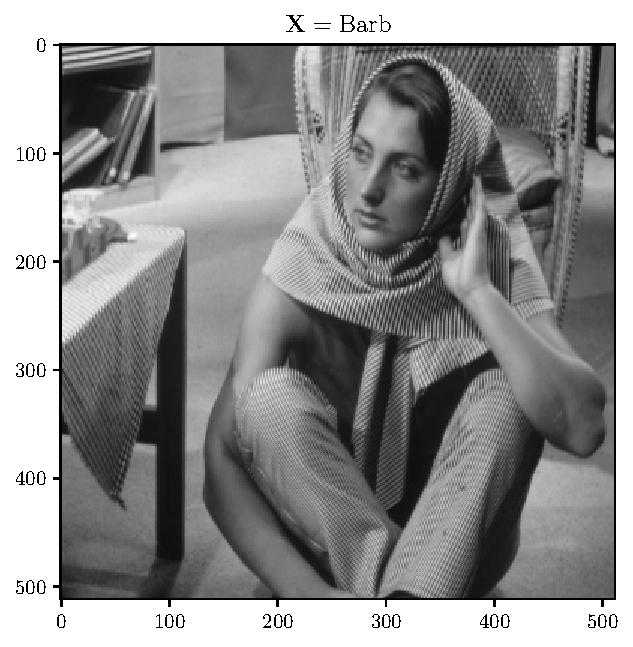
\includegraphics{barb.pdf}} & \href{https://nbviewer.org/github/vicente-gonzalez-ruiz/denoising/blob/main/notebooks/barb_0MMPG.ipynb\#barb_0MMPG}{\includegraphics{barb_0MMPG.pdf}} \\
      \href{https://nbviewer.org/github/vicente-gonzalez-ruiz/denoising/blob/main/notebooks/barb_averaging.ipynb\#barb_averaging}{\includegraphics{barb_averaging.pdf}} & \href{https://nbviewer.org/github/vicente-gonzalez-ruiz/denoising/blob/main/notebooks/barb_averaging_PSNR.ipynb\#barb_averaging_PSNR}{\includegraphics{barb_averaging_PSNR.pdf}}
    \end{tabular}
  }
  \caption{Increase of the SNR as a function of the number of noisy
    instances used in MNI. The clean image is shown on the top-left,
    and a noisy instance on the top-right. On the bottom-left, the
    denoised NMI image, and on the bottom-right the progression of the
    SNR as a function of $I$ and the level of
    noise.\label{fig:MNI_0MMPG}}
\end{figure}

\begin{comment}
%{{{

Fig.~\ref{fig:0MAUN} shows an
example of how zero-mean uniform noise is cancelled by averaging.
  
  \begin{figure}
    \centering
    \resizebox{1.0\textwidth}{!}{
      \renewcommand{\arraystretch}{0.0} % Adjust row spacing in the table
      \setlength{\tabcolsep}{0ex}      % Adjust column spacing in the table    
      \begin{tabular}{cc}
        \href{https://nbviewer.org/github/vicente-gonzalez-ruiz/denoising/blob/main/figs/averaging_denoising.ipynb\#Display-Barb}{\includegraphics{barb}} & \href{https://nbviewer.org/github/vicente-gonzalez-ruiz/denoising/blob/main/figs/averaging_denoising.ipynb\#0MAUN_barb}{\includegraphics{0MAUN_barb}} \\
        \href{https://nbviewer.org/github/vicente-gonzalez-ruiz/denoising/blob/main/figs/averaging_denoising.ipynb\#denoised_0MAUN_barb}{\includegraphics{denoised_0MAUN_barb}} & \href{https://nbviewer.org/github/vicente-gonzalez-ruiz/denoising/blob/main/figs/averaging_denoising.ipynb\#PSNR_0MAUN_barb}{\includegraphics{PSNR_0MAUN_barb}}
      \end{tabular}
    }
    \caption{Effect of zero-mean additive uniform noise in an image
      and how averaging can be used to reduced by averaging. The clean
      image of Barb is shown on the top left, and a noisy version on
      the top right. On to bottom, the left image shows a denoised
      version after averaging and the right graph shows the performance
      of the averaging process for different levels of
      noise.\label{fig:0MAUN}}
  \end{figure}

 Fig.~\ref{fig:0MAGN} shows an
  example of how zero-mean Gaussian noise is cancelled by averaging.

  \begin{figure}
    \centering
    \resizebox{1.0\textwidth}{!}{
      \renewcommand{\arraystretch}{0.0} % Adjust row spacing in the table
      \setlength{\tabcolsep}{0ex}      % Adjust column spacing in the table    
      \begin{tabular}{cc}
        \href{https://nbviewer.org/github/vicente-gonzalez-ruiz/denoising/blob/main/figs/averaging_denoising.ipynb\#barb}{\includegraphics{barb}} & \href{https://nbviewer.org/github/vicente-gonzalez-ruiz/denoising/blob/main/figs/averaging_denoising.ipynb\#0MAGN_barb}{\includegraphics{0MAGN_barb}} \\
        \href{https://nbviewer.org/github/vicente-gonzalez-ruiz/denoising/blob/main/figs/averaging_denoising.ipynb\#denoised_0MAGN_barb}{\includegraphics{denoised_0MAGN_barb}} & \href{https://nbviewer.org/github/vicente-gonzalez-ruiz/denoising/blob/main/figs/averaging_denoising.ipynb\#PSNR_0MAGN_barb}{\includegraphics{PSNR_0MAGN_barb}}
      \end{tabular}
    }
    \caption{Effect of zero-mean additive Gaussian noise in an image
      and how averaging can be used to reduced by averaging. The clean
      image of Barb is shown on the top left, and a noisy version on
      the top right. On to bottom, the left image shows a denoised
      version after averaging and the right graph shows the performance
      of the averaging process for different levels of
      noise.\label{fig:0MAGN}}
  \end{figure}

  Fig.~\ref{fig:0MMGN} shows an example of
  how zero-mean Gaussian noise is cancelled by averaging.

  \begin{figure}
    \centering
    \resizebox{1.0\textwidth}{!}{
      \renewcommand{\arraystretch}{0.0} % Adjust row spacing in the table
      \setlength{\tabcolsep}{0ex}      % Adjust column spacing in the table    
      \begin{tabular}{cc}
        \href{https://nbviewer.org/github/vicente-gonzalez-ruiz/denoising/blob/main/figs/averaging_denoising.ipynb\#barb}{\includegraphics{barb}} & \href{https://nbviewer.org/github/vicente-gonzalez-ruiz/denoising/blob/main/figs/averaging_denoising.ipynb\#0MMGN_barb}{\includegraphics{0MMGN_barb}} \\
        \href{https://nbviewer.org/github/vicente-gonzalez-ruiz/denoising/blob/main/figs/averaging_denoising.ipynb\#denoised_0MMGN_barb}{\includegraphics{denoised_0MMGN_barb}} & \href{https://nbviewer.org/github/vicente-gonzalez-ruiz/denoising/blob/main/figs/averaging_denoising.ipynb\#PSNR_0MMGN_barb}{\includegraphics{PSNR_0MMGN_barb}}
      \end{tabular}
    }
    \caption{Effect of zero-mean multiplicative Gaussian noise in an
      image and how averaging can be used to reduced by averaging. The
      clean image of Barb is shown on the top left, and a noisy
      version on the top right. On to bottom, the left image shows a
      denoised version after averaging and the right graph shows the
      performance of the averaging process for different levels of
      noise.\label{fig:0MMGN}}
  \end{figure}

 Fig.~\ref{fig:Rayleigh}
  shows an example of how Rayleigh noise is cancelled by averaging.

  \begin{figure}
    \centering
    \resizebox{1.0\textwidth}{!}{
      \renewcommand{\arraystretch}{0.0} % Adjust row spacing in the table
      \setlength{\tabcolsep}{0ex}      % Adjust column spacing in the table    
      \begin{tabular}{cc}
        \href{https://nbviewer.org/github/vicente-gonzalez-ruiz/denoising/blob/main/figs/averaging_denoising.ipynb\#barb}{\includegraphics{barb}} & \href{https://nbviewer.org/github/vicente-gonzalez-ruiz/denoising/blob/main/figs/averaging_denoising.ipynb\#Rayleigh_barb}{\includegraphics{Rayleigh_barb}} \\
        \href{https://nbviewer.org/github/vicente-gonzalez-ruiz/denoising/blob/main/figs/averaging_denoising.ipynb\#denoised_Rayleigh_barb}{\includegraphics{denoised_Rayleigh_barb}} & \href{https://nbviewer.org/github/vicente-gonzalez-ruiz/denoising/blob/main/figs/averaging_denoising.ipynb\#PSNR_Rayleigh_barb}{\includegraphics{PSNR_Rayleigh_barb}}
      \end{tabular}
    }
    \caption{Effect of Rayleigh noise in an image and how averaging can
      be used to reduced by averaging. The clean image of Barb is shown
      on the top left, and a noisy version on the top right. On to
      bottom, the left image shows a denoised version after averaging
      and the right graph shows the performance of the averaging
      process for different levels of noise.\label{fig:Rayleigh}}
  \end{figure}

  Fig.~\ref{fig:Poisson} shows an example of how Poisson noise is
  cancelled by averaging.

  \begin{figure}
    \centering
    \resizebox{1.0\textwidth}{!}{
      \renewcommand{\arraystretch}{0.0} % Adjust row spacing in the table
      \setlength{\tabcolsep}{0ex}      % Adjust column spacing in the table    
      \begin{tabular}{cc}
        \href{https://nbviewer.org/github/vicente-gonzalez-ruiz/denoising/blob/main/figs/averaging_denoising.ipynb\#barb}{\includegraphics{barb}} & \href{https://nbviewer.org/github/vicente-gonzalez-ruiz/denoising/blob/main/figs/averaging_denoising.ipynb\#Poisson_barb}{\includegraphics{Poisson_barb}} \\
        \href{https://nbviewer.org/github/vicente-gonzalez-ruiz/denoising/blob/main/figs/averaging_denoising.ipynb\#denoised_Poisson_barb}{\includegraphics{denoised_Poisson_barb}} & \href{https://nbviewer.org/github/vicente-gonzalez-ruiz/denoising/blob/main/figs/averaging_denoising.ipynb\#PSNR_Poisson_barb}{\includegraphics{PSNR_Poisson_barb}}
      \end{tabular}
    }
    \caption{Effect of Poisson noise in an image and how averaging can
      be used to reduced by averaging. The clean image is shown
      on the top left, and a noisy version on the top right. On the
      bottom, the left image shows a denoised version after averaging
      and the right graph shows the performance of the averaging
      process for different levels of noise.\label{fig:Poisson}}
  \end{figure}

%}}}
\end{comment}

%}}}

%}}}

\chapter{Gaussian Filtering (GF)}
%{{{

\section{Fourier transform of a Gaussian function}
\label{sec:FTGF}
%{{{

Let the Gaussian function defined by
\begin{equation}
  h(x) = \frac{1}{\sqrt{2\pi}\tau}e^{-\frac{{x}^2}{(2\tau^2)}},
  \label{eq:gaussian_ape}
\end{equation}
(see Eq.~\ref{eq:GF}), the Fourier transform  is
\begin{equation}
  H(w) = \mathcal{F}\{h(x)\} = \int_{-\infty}^{\infty}h(x)e^{-jwx}dx,
\end{equation}
where
\begin{equation}
  w = 2\pi f,
\end{equation}
representing $f$ frequency (in the case of working with images, in
cycles per pixel-size measured in units of distance, or simply, cycles
per sample) and $w$ angular frequency (radians per unit distance, or
simply, radians per sample). Therefore,
\begin{equation*}
  H(w) = \int_{-\infty}^{\infty}\frac{1}{\sqrt{2\pi}\tau}e^{-\frac{x^2}{2\tau^2}}e^{-jwx}dx = 
\end{equation*}
\begin{equation*}
  \frac{1}{\sqrt{2\pi}\tau}\int_{-\infty}^{\infty}e^{-\frac{x^2}{2\tau^2}}e^{-jwx}dx = 
\end{equation*}
\begin{equation*}
  \frac{1}{\sqrt{2\pi}\tau}\int_{-\infty}^{\infty}e^{-\frac{x^2}{2\tau^2}-jwx}dx.
\end{equation*}
Operating in the exponent
\begin{equation*}
  -\frac{x^2}{2\tau^2}-jwx = -\frac{1}{2\tau^2}(x+2j\tau^2wx)
\end{equation*}
that after adding and subtracting $(j\tau^2w)^2$
\begin{equation*}
  = \frac{1}{2\tau^2}[(x+j\tau^2w)^2-(j\tau^2w)^2]
\end{equation*}
and rewriting and operating
\begin{equation*}
  = -\frac{(x+j\tau^2w)^2}{2\tau^2} + \frac{\tau^2w^2}{2}.
\end{equation*}
Replacing the exponent,
\begin{equation*}
  H(w) = \frac{1}{\sqrt{2\pi}\tau}e^{-\frac{\tau^2w^2}{2}}\int_{-\infty}^{\infty}e^{-\frac{(x+j\tau^2w)^2}{2\tau^2}}dx.
\end{equation*}
Now define
\begin{equation*}
  u = x + j\tau^2w.
\end{equation*}
Therefore,
\begin{equation*}
  H(w) = \frac{1}{\sqrt{2\pi}\tau}e^{-\frac{\tau^2w^2}{2}}\int_{-\infty}^{\infty}e^{{-u^2}{2\tau^2}}du.
\end{equation*}
The remaining integral is a standard Gaussian integral,
\begin{equation*}
  \int_{-\infty}^{\infty}e^{{-u^2}{2\tau^2}}du = \sqrt{2\pi}\tau.
\end{equation*}
Finally, we obtain that
\begin{equation}
  H(w) = e^{-\frac{\tau^2w^2}{2}},
  \label{eq:FTGF}
\end{equation}
that corresponds to the transfer function (i.e., the response of
Eq.~\ref{eq:gaussian_ape} to the impulse signal) of the Gaussian.

%}}}

\section{Cut-off frequency of a Gaussian filter}
\label{sec:tau_VS_eta}
%{{{

Gaussian filters are low-pass filters. In a low-pass filter we can
distinguish three subbands: (1) the pass-band, that is defined by
those range of frequencies that are not attenuated significantly, (2)
the stop-band, where the frequencies are attenuated (significantly),
and (3) the transition-band, defined by those frequencies that are not
included in the previous subbands. Notice that only in an ideal
filter, the size of the transition-band is zero.

The cut-off frequency of a low-pass filter is defined by those
frequencies of the transition-band where the response (or gain) of the
filter decreases by some given factor $\beta\in]0,1[$. In other words,
if $H$ is the transfer function of the filter,
\begin{equation}
  H(\eta) = \beta,
\end{equation}
where $\eta$ is the cut-off frequency. In the case of a Gaussian
filter (see Eq.~\ref{eq:FTGF}), we have that
\begin{equation*}
  H(\eta) = e^{-\frac{\tau^2\eta^2}{2}} = \beta.
\end{equation*}
Taking the natural logarithm
\begin{equation*}
  -\frac{\tau^2\eta^2}{2} = \ln\beta.
\end{equation*}
Solving for $\tau$
\begin{equation}
  \tau = \frac{\sqrt{-2\ln\beta}}{\eta}.
  \label{eq:tau_VS_eta}
\end{equation}

Typically, $\beta=1/\sqrt{2}$ that is equivalent to attenuate the
input signal in -3dB. Notice that at the frequency 0 (see
Eq.~\ref{eq:FTGF}),
\begin{equation*}
  H(0) = e^0=1.
\end{equation*}

Eq.~\ref{eq:tau_VS_eta} uses angular frequency. We can obtain the
corresponding expresión for ``standard'' frequency, knowing that
\begin{equation}
  \eta = 2\pi\hat{\eta}.
  \label{eq:eta_freq}
\end{equation}
Using Eq.~\ref{eq:eta_freq} into Eq.~\ref{eq:tau_VS_eta}, we obtain
\begin{equation}
  \tau = \frac{\sqrt{-2\ln\beta}}{2\pi\hat{\eta}}.
  \label{eq:tau_VS_eta_standard}
\end{equation}
Operating
\begin{equation*}
  \frac{\sqrt{-2\ln\beta}}{2\pi\hat{\eta}} = \frac{\sqrt{2}\sqrt{-\ln\beta}}{2\pi\hat{\eta}} = \frac{\sqrt{2}\sqrt{-\ln\beta}}{2\pi\hat{\eta}}\frac{\sqrt{2}}{\sqrt{2}} = \frac{2\sqrt{-\ln\beta}}{2\sqrt{2}\pi\hat{\eta}} = \frac{\sqrt{-\ln\beta}}{\sqrt{2}\pi\hat{\eta}},
\end{equation*}
and therefore,
\begin{equation}
  \hat{\tau} = \frac{\sqrt{-\ln\beta}}{\sqrt{2}\pi\hat{\eta}},
  \label{eq:ideal_hat_tau}
\end{equation}
equation that is valid for continuous signals. In the discrete case,
where the Gaussian kernel is finite in length, we have that
\begin{equation}
  \mathbf{h}.\mathsf{size} = 2\lceil k\tau\rceil + 1,
  \label{eq:kernel_length}
\end{equation}
i.e., the filter is truncated at $\pm k\tau$ coefficients. This has
two effects (obviously, if $\tau$ remains constant):
\begin{enumerate}
\item If $k$ is small, the attenuation of the stop-band decreases,
  i.e., the performance of the filter is worse (see
  Fig.~\ref{fig:gaussian_leakage}). Therefore, $k$ should be big
  enought.
\item But if $k$ is to big, and we desire a $\hat{\eta}$ (the cut-off
  frequency) high because the SNR is only low above $\hat{\eta}$, we
  will perform a low of multiplications which results in values very
  close to zero, increasing the computation time without showing
\end{enumerate}
Therefore, a better estimation of the standard deviation for the
Gaussian kernel is
\begin{equation}
  \tau = \frac{\sqrt{-\ln\beta}}{\sqrt{2}\pi\hat{\eta}k}.
  \label{eq:ideal_hat_tau}
\end{equation}

\begin{figure}
  \centering
  \href{https://nbviewer.org/github/vicente-gonzalez-ruiz/denoising/blob/main/notebooks/gaussian_leakage.ipynb\#Gaussian_leakage}{\includegraphics[width=0.8\textwidth]{gaussian_leakage}}
  \caption{Impact of $k$ in the frequency response of a digital
    Gaussian kernel, when $k$ and $\tau$ are related according
    to Eq.~\ref{eq:kernel_length}). The lobes in the stop-band are
    generated by the convolution of the ideal frequency response of a
    ideal (continous) Gaussian filter (see Eq.~\ref{eq:FTGF}) with the
    Fourier transform of the square function which mathematically
    models the truncation in length of the kernel. $f_s$ represents
    the sampling frequency.\label{fig:gaussian_leakage}}
\end{figure}

For $k=4$, the attenuation of the stop-band is below $90\text{dB}$
(see Fig.~\ref{fig:gaussian_leakage}) and the leakage generated by the
truncation remains low enough.

Finally, to assert the correctness of Eq.~\ref{eq:ideal_hat_tau}, we
have computed the relation between $\tau$ and $\hat{\eta}$ for
$\beta=1/\sqrt{2}$, and the result has been plotted in the
Fig.~\ref{fig:eta_vs_tau}. As can be seen, $\tau\propto 1/\hat{\eta}$.

\begin{figure}
  \centering
  \href{https://nbviewer.org/github/vicente-gonzalez-ruiz/denoising/blob/main/notebooks/eta_vs_tau.ipynb\#Eta_vs_tau}{\includegraphics[width=0.8\textwidth]{eta_vs_tau}}
  \caption{Relation between $\hat\eta$ (the digital cut-off frequency
    of a Gaussian kernel) and $\tau$ (the standard deviation of
    the kernel), for $\beta=1/\sqrt{2}$.\label{fig:eta_vs_tau}}
\end{figure}

\begin{comment}
To convert to normalized frequency, we must divide by $f_s$, the
sampling frequency. For example, if $f_s=1$, we are supposing one
sample per unit distance.
\end{comment}

\begin{comment}
Now, if we are using digital signals, where the frequency is
normalized relative to Nyquist frequency, we have that

and continuous signals. In the digital world the Gaussian
kernel is finite and this must be also considered to find the cut-off
frequency. In our implementation, that is based on the method
\href{https://docs.scipy.org/doc/scipy/reference/generated/scipy.ndimage.gaussian_filter1d.html}{scipy.ndimage.gaussian\_filter1d()},
\begin{equation}
  \mathbf{h}.\mathsf{size} = 2\lceil k\tau\rceil + 1,
\end{equation}
where $k=4$ provides enough accuracy in the
convolutions.\footnote{Notice that if $k$ grows then the cut-off
  frequency of the filter decreases, regardless of $\tau$.}
\end{comment}
\begin{comment}
In those denoising algorithms where we can estimate the optimal
filtering parameters ($\tau^*$ in the case of GF) considering the
information of the signal in the frequency domain, a relation between
$\tau$ and the cut-off frequency $\eta$ of the filter is
required. Such relation can be found after defining an attenuation
threshold $\beta\in [0,1]$, and determining for which increasing value
of $\eta$ the gain of the low-pass filter in the frequency domain is
below $\beta$.
\end{comment}

%}}}

%{{{

\begin{comment}
\section{Transfer function of a Gaussian filter}
%{{{

\label{sec:transfer_function_GK}

The transfer function of a filter (kernel) is the Fourier transform of the
impulse response of the filter,
\begin{equation}
  H(w) = \mathcal{F}\{h(x)\} = \int_{-\infty}^{\infty}h(x)e^{-jwx}dx.
\end{equation}
Using the Fourier pair
\begin{equation}
  \mathcal{F}\{e^{-\frac{x^2}{2\tau^2}}\} = \tau\sqrt{2\pi}e^{-\frac{\tau^2x^2}{2}},
\end{equation}
we get that
\begin{equation}
  H(w) = e^{-\frac{\tau^2w^2}{2}}.
  \label{eq:TFGK}
\end{equation}

%}}}
\end{comment}

%}}}

\section{About separability in multidimensional GF}
\label{sec:GF_separability}
%{{{

A 2D function $f(x,y)$ is said to be separable if can be expressed as
the product of 2 1D functions. Thus, a $D$-dimensional Gaussian
filtering can be computed applying a 1D Gaussian filter along each of
the $N$ dimensions. This reduces the computational complexity from
$\mathcal{O}(N^D)$ to $D\mathcal{O}(N)$, where $N$ is the problem
size.

In the case of 2D Gaussian filtering, the kernel is defined by
\begin{equation}
  h(x,y) = \frac{1}{2\pi\tau^2}e^{-\frac{x^2+y^2}{2\tau^2}},
  \label{eq:2DGF}
\end{equation}
where $\tau$ is the standard deviation. Since
\begin{equation*}
  e^{-\frac{x^2+y^2}{2\tau^2}} = e^{-\frac{x^2}{2\tau^2}}e^{-\frac{y^2}{2\tau^2}},
\end{equation*}
then
\begin{equation}
  h(x,y) = \Big(\frac{1}{\sqrt{2\pi}\tau}e^{-\frac{x^2}{2\tau^2}}\Big)\Big(\frac{1}{\sqrt{2\pi}\tau}e^{-\frac{y^2}{2\tau^2}}\Big) = f(x)g(y),
\end{equation}
where
\begin{equation}
  f(x) = \frac{1}{\sqrt{2\pi}\tau}e^{-\frac{x^2}{2\tau^2}},
\end{equation}
and equivalently for $g(y)$.

Alternatively, in the Fourier domain
\begin{equation*}
  \begin{split}
    H(u,v) & = \int_\infty^\infty\int_\infty^\infty h(x,y)e^{-2\pi j(ux+vy)}dxdy \\
           & = \int_\infty^\infty\int_\infty^\infty f(x)g(y)e^{-2\pi j(ux)}e^{-2\pi j(vy)}dxdy \\
           & = \int_\infty^\infty f(x)e^{-2\pi j(ux)} dx \int_\infty^\infty g(y) e^{-2\pi j(vy)} dy \\
           & = F(u)G(v).
  \end{split}
\end{equation*}
Therefore, the frequency response of a separable multidimensional
filter can be found by multipliying the frequency responses in each
dimension of the corresponding 1D filter. Notice that this is a
general result, known as The Separability Theorem.

In terms of a 2D digital isotropic filter, if $w$ is its (2D) kernel,
separability implies that it can be expressed as the outer product
\cite{gonzalez1992digital}
\begin{equation}
  w = vv^T,
\end{equation}
where $v$ is a 1D kernel. Notice also that, as a consequence of this,
the $\text{rank}(w)=1$.

%}}}


\section{Gaussian denoising}
%{{{

Gaussian denoising is based on the use of low-pass
(smoothing)\footnote{Because random noise typically consists of sharp
  transitions in intensity, an obvious application of smoothing is
  noise reduction \cite{gonzalez1992digital}.} Gaussian
filters. Unlike other digital filters, such as an ideal low-pass
filter, a Gaussian low-pass filter does not generate ringing (the
transfer function of a Gaussian filter is another Gaussian filter,
which has not lobes), and the convolution of two Gaussians are Gaussian
functions also. 

In GF denoising, a 1D Gaussian kernel $\mathbf{h}$ is convolved with
the noisy instance $\hat{\mathbf{X}}$ to obtain
\begin{equation}
  \tilde{\mathbf{X}} = \hat{\mathbf{X}}*\mathbf{h},
  \label{eq:GF}
\end{equation}
where $\tilde{\mathbf{X}}$ represents the denoised signal, and $*$ the
convolution between digital signals. As can be seen, unlike MNI, GF
requires only one instance.

The coefficients of $\mathbf{h}$ define a low-pass\footnote{We can
  distinguish this because all are positive coefficients.}
filter, which are sampled from
\begin{equation}
  h(x) = \frac{1}{\sqrt{2\pi}\tau}e^{-\frac{{x}^2}{(2\tau^2)}},
  \label{eq:GK}
\end{equation}
where $x$ represents a distance in
the signal domain, and $\tau$ (known as the \emph{standard deviation}
\footnote{Notice that the filter coefficients are also the values that a
  discrete random variable takes from a normal distribution.})
determines the bandwidth of the filter.

\begin{figure}
  \centering
  \includegraphics[width=0.8\textwidth]{3D_GF}
  \caption{3D Gaussian filtering. The gray planes contain the voxels
    that are filtered and the white planes contain the voxels used by
    the 1D kernel when it is applied to the voxels of the filtered
    plane. The kernel shown here contains 3 coefficients. The volume
    is convolved sequentially in-place, from left to
    right.\label{fig:3D_GF}}
\end{figure}

Multidimensional GF is separable (see
Appendix~\ref{sec:GF_separability}), which means that we can apply the
1D filter to the $D$ dimensions of the signal to compute a $D$D
denoising. De facto, Gaussian kernels are the only circularly
symmetric kernels that are also separable
\cite{gonzalez1992digital}. For the 3D case (see
Fig.~\ref{fig:3D_GF}), we have that
\begin{equation}
  \tilde{\mathbf{X}} = \Big(\big(\hat{\mathbf X}*^{(\text{Z})}{\mathbf h}\big)*^{(\text{Y})}{\mathbf h}\Big)*^{(\text{X})}{\mathbf h},
    \label{eq:3D_GF}
\end{equation}
where ${\mathbf s}*^{(d)}{\mathbf h}$ is the 1D convolution applied to
the dimension $d$ of the signal ${\mathbf s}$ and the (1D) kernel
${\mathbf h}$. For simplicity, Eq.~\ref{eq:3D_GF} defines isotropic
filtering, but $\tau$ can be different at each dimension to provide
anisotropy. Eq.~\ref{eq:3D_GF} is implemented
\href{https://github.com/vicente-gonzalez-ruiz/denoising/blob/main/src/denoising/volume/gaussian.py}{here},
and the corresponding 2D version is implemented
\href{https://github.com/vicente-gonzalez-ruiz/denoising/blob/main/src/denoising/image/gaussian.py}{here}.

\begin{comment}
%{{{

 This idea has been describen in Python pseudo-code in
the Fig.~\ref{fig:3DGF_imple}.

\begin{figure}
\noindent $\mathsf{3DGF}(\hat{\mathbf{X}}, \mathbf{h})$: $\rightarrow\tilde{\mathbf{X}}$
\vspace{-1ex}
\begin{enumerate}
  \setlength{\itemsep}{0pt}
\item [1.] $\tilde{\mathbf{X}}\leftarrow\href{https://docs.opencv.org/2.4/modules/imgproc/doc/geometric_transformations.html#resize}{\mathsf{resize}}(\hat{\mathbf{X}}, \mathsf{dsize}=)$
\item [2.] $\mathsf{for}~z~\mathsf{in}~\mathsf{range}(\hat{\textbf{X}}.\mathsf{shape}_0),~\mathsf{run}$:  \hfill $\mathtt{/*~Filtering~in~the~Z~direction~*/}$
  \begin{enumerate}
  \item [1.] $\mathsf{for}~h~\mathsf{in~range}(\mathbf{h}.\mathsf{size})$:
    \begin{enumerate}
    \item [1.] $\tilde{\mathbf{X}}_{z,:,:}\leftarrow\tilde{\mathbf{X}}_{z,:,:}+\hat{\mathbf{X}}_{z,:,:}\mathbf{h}_{h}$
    \end{enumerate}
  \end{enumerate}
\item [3.] $\mathsf{for}~y~\mathsf{in}~\mathsf{range}(\hat{\textbf{X}}.\mathsf{shape}_1),~\mathsf{run}$:  \hfill $\mathtt{/*~Filtering~in~the~Y~direction~*/}$
  \begin{enumerate}
  \item [1.] $\mathsf{for}~k~\mathsf{in~range}(\mathbf{h}.\mathsf{size})$:
    \begin{enumerate}
    \item [1.] $\tilde{\mathbf{X}}_{:,y,:}\leftarrow\tilde{\mathbf{X}}_{:,y,:}+\hat{\mathbf{X}}_{:,y,:}\mathbf{h}_{h}$
    \end{enumerate}
  \end{enumerate}
\item [4.] $\mathsf{for}~x~\mathsf{in}~\mathsf{range}(\hat{\textbf{X}}.\mathsf{shape}_2),~\mathsf{run}$:  \hfill $\mathtt{/*~Filtering~in~the~X~direction~*/}$
  \begin{enumerate}
  \item [1.] $\mathsf{for}~h~\mathsf{in~range}(\mathbf{h}.\mathsf{size})$:
    \begin{enumerate}
    \item [1.] $\tilde{\mathbf{X}}_{:,:,x}\leftarrow\tilde{\mathbf{X}}_{:,:,x}+\hat{\mathbf{X}}_{:,:,x}\mathbf{h}_{h}$
    \end{enumerate}
  \end{enumerate}
\end{enumerate}
%\end{myquote}
\caption{Python pseudo-code of 3DGF using periodic signal extension.}
\label{fig:3DGF_imple}
\end{figure}

%}}}
\end{comment}

\begin{figure}
  \centering
  \resizebox{1.0\textwidth}{!}{
    \renewcommand{\arraystretch}{0.0} % Adjust row spacing in the table
    \setlength{\tabcolsep}{0ex}      % Adjust column spacing in the table    
    \begin{tabular}{cc}
      %\href{https://nbviewer.org/github/vicente-gonzalez-ruiz/denoising/blob/main/notebooks/barb.ipynb}{\includegraphics{barb}} & \href{https://nbviewer.org/github/vicente-gonzalez-ruiz/denoising/blob/main/figs/lake.ipynb}{\includegraphics{lake}} \\
      %\href{https://nbviewer.org/github/vicente-gonzalez-ruiz/denoising/blob/main/notebooks/barb_0MMPG.ipynb}{\includegraphics{barb_0MMPG}} & \href{https://nbviewer.org/github/vicente-gonzalez-ruiz/denoising/blob/main/notebooks/lake_0MMPG.ipynb}{\includegraphics{lake_0MMPG}} \\
      \href{https://nbviewer.org/github/vicente-gonzalez-ruiz/denoising/blob/main/notebooks/Confocal_FISH_GF_optimal_tau.ipynb\#Confocal_FISH_GF_optimal_tau}{\includegraphics{Confocal_FISH_GF_optimal_tau.pdf}} & \href{https://nbviewer.org/github/vicente-gonzalez-ruiz/denoising/blob/main/notebooks/TwoPhoton_MICE_GF_optimal_tau.ipynb\#TwoPhoton_MICE_GF_optimal_tau}{\includegraphics{TwoPhoton_MICE_GF_optimal_tau.pdf}}
    \end{tabular}
  }
  \caption{Optimal $\tau$ values in GF.\label{fig:optimal_GF_tau}}
\end{figure}

As can be seen in Eq.~\ref{eq:GK}, the denoising result depends on
$\tau$. An optimal value for the standard deviation, $\tau^*$, can be
found if we know $\mathbf{X}$ (see
Fig.~\ref{fig:optimal_GF_tau}). Unfortunately, $\mathbf{X}$ is usually
unknown and we only can estimate $\tau^*$. Ideally, $\tau^*$ should
increase the SNR as much as possible, considering also that: (1) GF
attenuates the high frequencies, (2) the SFC of the noise is close to
zero, and (3) that most of the energy (information) in the signals are
concentrated in the low frequencies. Therefore, we should find a
cut-off frequency
\begin{equation}
  \eta^* = \text{min}\{\eta|\text{SFC}(\hat{\mathbf{X}})_\eta < \alpha\},
  \label{eq:search_eta}
\end{equation}
where $\alpha$ is the minimun correlation that should reach the SFC to consider that the corresponding ring/shell has a high enough SNR (see
Appendix~\ref{sec:tau_VS_eta}). Once we have already estimated
$\eta^*$, we can use the corresponding $\tau^*$ to filter out those
frequency components of $\hat{\mathbf{X}}$ with the lowest SNR.

\begin{figure}
  \centering
  \resizebox{1.0\textwidth}{!}{
    \renewcommand{\arraystretch}{0.0} % Adjust row spacing in the table
    \setlength{\tabcolsep}{0ex}      % Adjust column spacing in the table    
    \begin{tabular}{cc}
      \href{https://nbviewer.org/github/vicente-gonzalez-ruiz/denoising/blob/main/notebooks/Confocal_FISH_GF_estimation.ipynb}{\includegraphics{Confocal_FISH_GF_estimation.pdf}} & \href{https://nbviewer.org/github/vicente-gonzalez-ruiz/denoising/blob/main/notebooks/TwoPhoton_MICE_GF_estimation.ipynb}{\includegraphics{TwoPhoton_MICE_GF_estimation.pdf}}
    \end{tabular}
  }
  \caption{Optimal VS estimated $\tau^*$ values.\label{fig:tau_GF_estimation}}
\end{figure}

In the Fig.~\ref{fig:tau_GF_estimation} there is a comparison between
the true $\tau^*$ values and their estimations, using the EOS
technique (see Appendix~\ref{sec:EOS}) to compute the SFC curves (see
Section~\ref{sec:fourier_correlation}). Specifically, we have used
(see Eq.~\ref{eq:ideal_hat_tau} and Fig.~\ref{fig:eta_vs_tau})
\begin{equation}
  \tau^*_{\text{EOS}} = \frac{0.141}{2\eta^*},
  \label{eq:tau_VS_eta_empirical_EOS}
\end{equation}
(and not exactly the fitting expression shown in the
Fig.~\ref{fig:gaussian_leakage}) because using signal splitting to
compute the SFC, only the first half of the frequencies provide
reliable information. Notice that, to determine $\eta^*$ (the
estimated ``optimal'' cut-off frequency of the Gaussian filter) we
have assumed that an attenuation higher than $1/\sqrt{2}$ (see
Appendix~\ref{sec:tau_VS_eta}) can be high enought to filter out the
frequencies higher than $\eta^*$.

Appendix~\ref{sec:results} contains a table with the performance of
some denoisers.

%{\color{red} Podemos comparar diferentes algoritmos de denoising si usamos, para una determinada configuración de ruido, el filtrado óptimo (que es posible encontrar porque tenemos el GT). Nos va a salir una tabla con valores de PCC.}

%Since all denoising algorithms have a similar behavior (they tend to
%eliminate high frequencies and preserve low ones), we will consider
%Eq.~\ref{eq:tau_VS_eta_empirical_EOS} as generic and it will be used
%to find the optimal value of the different operating parameters of the
%denoising algorithms.

\begin{comment}
%{{{

Concretelly, we use (see
Appendix~\ref{SFC_random_data})
\begin{equation}
  \tau^*_{\text{SPRS}} = \frac{0.141}{5(\eta^*-0.09)},
  \label{eq:tau_VS_eta_empirical_SPRS}
\end{equation}
when we are using the SPRS algorithm to find the SFC curve, or
\begin{equation}
  \tau^*_{\text{EO}} = \frac{0.141}{3(\eta^*-0.01)},
  \label{eq:tau_VS_eta_empirical_EO}
\end{equation}
if we are using the EO algorithm to find the SFC curve,
where we are supposing that $\beta=1/\sqrt{2}$ (see
Appendix~\ref{sec:tau_VS_eta}). 

Fig.~\ref{fig:tau_GF_estimation} shows the result of using
Eqs.~\ref{eq:tau_VS_eta_empirical_SPRS} and
\ref{eq:tau_VS_eta_empirical_EO} for estimating $\tau^*$ for the two
test images. As can be seen ..

%}}}
\end{comment}

\begin{comment}
%{{{

Assuming that most of the signal energy (information) is concentrated
in the low frequencies, higher values of $\tau$ will produce a higher
smoothing effect in $\tilde{\mathbf{X}}$). More concretely, if
$\mathcal{F}(h)=H$, that is
\begin{equation}
  H(u) = e^{-\frac{u^2}{2\tau^{-2}}},
\end{equation}
it can be seen that if $\tau$ increases, the cut-off frequency
provided by $H$ decreases, and viceversa. 


\begin{figure}
  \centering
  \resizebox{1.0\textwidth}{!}{
    \renewcommand{\arraystretch}{0.0} % Adjust row spacing in the table
    \setlength{\tabcolsep}{0ex}      % Adjust column spacing in the table    
    \begin{tabular}{cc}
      \href{https://nbviewer.org/github/vicente-gonzalez-ruiz/denoising/blob/main/notebooks/barb.ipynb}{\includegraphics{barb}} & \href{https://nbviewer.org/github/vicente-gonzalez-ruiz/denoising/blob/main/figs/lake.ipynb}{\includegraphics{lake}} \\
      \href{https://nbviewer.org/github/vicente-gonzalez-ruiz/denoising/blob/main/notebooks/tau_VS_img.ipynb\#0MMPG_barb}{\includegraphics{0MMPG_barb}} & \href{https://nbviewer.org/github/vicente-gonzalez-ruiz/denoising/blob/main/figs/tau_VS_img.ipynb\#0MMPG_lake}{\includegraphics{0MMPG_lake}} \\
      \href{https://nbviewer.org/github/vicente-gonzalez-ruiz/denoising/blob/main/notebooks/tau_VS_img.ipynb\#GF_0MMPG_barb}{\includegraphics{GF_0MMPG_barb}} & \href{https://nbviewer.org/github/vicente-gonzalez-ruiz/denoising/blob/main/figs/tau_VS_img.ipynb\#GF_0MMPG_lake}{\includegraphics{GF_0MMPG_lake}}
    \end{tabular}
  }
  \caption{Two examples of optimal denoising using GF. On the top, the
    original images. In the middle, the noisy instances. On the
    bottom, the denoised images. {\color{red} arreglar PSNRs y elegir
      tau optimo para ejemplo}\label{fig:GF_tau_optimal}}
\end{figure}

Fig.~\ref{fig:tau_VS_image} shows the denoising performance of GF for
two artificially noised images, for different levels of noise
($\sigma$) and filter length ($\tau$). As can be seen, the optimal
value of the filter length, $\tau^*$ (which maximizes the PCC between
$\mathbf{X}$ and $\tilde{\mathbf{X}}$), depends on the noise level and
$\mathbf{X}$, information that is, in general, unavailable in
microscopy imaging. Therefore, $\tau^*$ can be only
\emph{estimated}\footnote{Notice that, only knowing $\mathbf{X}$ it
  would be possible to find $\tau^*$. Therefore, the furthest one can
  go is to estimate the optimal filtering parameters}. depending on,
for example, the (subjective) visual quality of
$\tilde{\mathbf{X}}$. An example of optimal denoising using GF has
been show in Fig.~\ref{fig:GF_tau_optimal}.

% \begin{figure}
%   \centering
%   \resizebox{1.0\textwidth}{!}{
%     \renewcommand{\arraystretch}{0.0} % Adjust row spacing in the table
%     \setlength{\tabcolsep}{0ex}      % Adjust column spacing in the table    
%     \begin{tabular}{cc}
%   \href{https://nbviewer.org/github/vicente-gonzalez-ruiz/denoising/blob/main/figs/gaussian_denoising.ipynb\#GD_SFRC_0MMPG_NL20_barb}{\includegraphics{GD_SFRC_0MMPG_NL20_barb}} & \href{https://nbviewer.org/github/vicente-gonzalez-ruiz/denoising/blob/main/figs/gaussian_denoising.ipynb\#GD_SFRC_0MMPG_NL60_barb}{\includegraphics{GD_SFRC_0MMPG_NL60_barb}}
%     \end{tabular}
%     }
%     \caption{SFRC curves for two different noisy instances of
%       Barb, see Fig.~\ref{fig:tau_VS_image} using two
%       different noise levels ($\sigma=20$ and $\sigma=60$), and after
%       having applied GD for several filter lengths. As can be seen, for $\sigma=20$, the ``optimal'' filter
%       length (that maximizes the area below the curve) is ..., and for
%       $\sigma=60$, the ``optimal'' filter length is ... Therefore, the
%       ``optimal'' filter length is (positively) correlated with the
%       noise level. Notice that $\tau$
%       has been discretized in steps of $0.25$.

%       (2) the
%       ``optimal'' filter length is (positively) correlated with the
%       noise level (for the noise level $\sigma=40$ and $\gamma=0.15$
%       the ``optimal'' $\tau=1.0$ and the noise level $\sigma=50$ and
%       $\gamma=0.15$ the ``optimal'' $\tau=1.25$). Notice that $\tau$
%       has been discretized in steps of $0.25$.


%       Relation between the SFRC curves and the filter length of
%       a Gaussian filter. $\hat{\mathbf{X}}_1$ is the the noise image
%       (Barb) shown in the Fig.~\ref{fig:tau_VS_image} (for $\sigma=40$
%       and $\gamma=0.15$). As can be seen, the area below the curve is
%       maximized for $\tau=1.0$

%       Effect of zero-mean MPG noise in an image and how GD
%     can be used to reduce it. A noisy version of the
%     image is on the top-left. On the top-right, the SFRC curves
%     of the denoised image for different filter lengths. As can be seen
%     in this subfigure, for the noise level
%     $(\sigma=40, \gamma=0.15)$, an optimal $\tau=1.25$ should be used if
%     (considering that the area below the SFRC curve should be maximized).
%     On the bottom-left, it can be seen that for this noise level,
%     the ``optimal'' Gaussian kernel-lenght is $\tau/2=0.625 \approx 0.7$. The resulting
%     ``optimal'' filtered image (using GD) is shown on the bottom-right.
%     \label{fig:GD_0MMPG}}
% \end{figure}

{\color{red} ------ comienzo sin terminar ------ }

It is also possible to estimate $\tau^*$ using the self-correlation in
the Fourier domain \cite{koho2019fourier} {\color{red}Este sería un
  buen punto para hablar de cómo estamos calculando la curva
  SF{R|S}C}. The idea here is to determine the frequency $u^*$ for
which, to the right of this frequency, the SNR decays under some given
threshold.

A more objective procedure to estimate $\tau^*$ should be based on
some (objective) quality metric, such as the self-correlation in the
Fourier domain \cite{koho2019fourier}. Fig.~\ref{fig:GD_0MMPG} shows
the result of using the SFRC of the noisy image to estimate $\tau^*$,
considering the idea that the low-pass filter should remove those
frequency components where the SNR is lower than a given threshold.



Fig.~\ref{fig:GD_0MMPG} shows
SFRC curves for different filter lengths, and it has been also
computed the normalized area below each curve, a metric that is
(positively) correlated with $\tau^*$ (see
Fig.~\ref{fig:tau_VS_image}). As can be seen that, $\tau^*$ can be
estimated using the filter length that maximizes the area below the
corresponding SFRC curve.


because the
higher the area, the higher also the PCC between the Fourier
coefficients


and it can be seen, the normalized area below the curve can be used to estimate


Another alternative can use some heuristic to estimate

We propose a more automatic procedure to find $\tau^*$.  by maximizing
the ratio between the amount of noise and the amount of signal removed
by the filter. To determine this, we can use the SFRC curve (see
Sec.~\ref{sec:FSC}), in which each point represents the correlation
between two\footnote{Actually, each point is the average (arithmetic
  mean) of two correlation coefficients, each one obtained after
  subsampling the image in each dimension (by rows, and by columns).}
rings of Fourier coefficients, extracted from two subsampled versions
of $\tilde{\mathbf{X}}$.

for the single parameter that GD requires (the length of
the Gaussian kernels in each dimension, represented by $\tau$ in
$\mathrm{GD}_\tau$) depends on the noise level, an information that is
generally unknown in microscopy imaging.

To estimate the relation between the filter length that should
maximize the quality of the denoised signal, the SFRC (Self Fourier
Ring Correlation, see Section~\ref{sec:FSC}) of several noisy
instances of the same image (variying the level of noise) has been
shown in the Fig.~\ref{fig:SFRC}.

has been calculated by subbands of a filtered
image, generating a number of SFRC curves, one for each different
kernel length $\tau$ (see Fig.  \ref{fig:GD_0MMPG}). As can be seen,
the autocorrelation increases when the noise level decreases due to
increasing $\tau$, until it reaches a value for which the
autocorrelation decreases again\footnote{Remember that the SFRC metric
  quantifies the correlation between subsampled versions of the same
  input signal and that, by definition, the MPG noise should be
  uncorrelated. For this reason, if noise were only had at the input,
  we should obtain a flat SFRC that approximates to zero. Therefore,
  the higher the area below the SFRC curve, the higher the presence of
  signal.}. For that $\tau^*$, which maximizes the area under the
curve up to the normalized frequency $\omega/4$, is when the PCC
metric is also maximized (considering the original image resolution,
i.e., without the subsampling required to compute the SFRC) for
$\tau^*/2$, which means that we can use the SFRC metric (in the 2D
case) and the SFSC (in the 3D case) to estimate the optimal filtering
parameters knowing only the noisy instance $\hat{\mathbf{X}}$.

{\color{red} ------ fin sin terminar ------ }

%}}}
\end{comment}

%}}}

%}}}


% \chapter{Beltrami flow}
% Parece que se usa en AND, pero no se bien cómo.

%\chapter{Median filter}

%\chapter{Bilateral filter}

\chapter{Wiener Filtering (WF)}
%{{{

The Wiener filter \cite{wiener1942extrapolation} is an adaptive linear
filter designed to minimize the MSE between the denoised signal
$\tilde{\mathbf{s}}$ and the \gls{GT} $\mathbf{s}$, when this has been
corrupted by noise\footnote{A Wiener filter also considers that
  $\mathbf{x}$ can be affected, apart from the noise, by some linear
  transformation (such as a blurring), but we will ingnore this.}. For
this reason, \gls{WF} is also known by \emph{minimum \gls{MSE} filtering} and also
by \emph{least square error fitering}. When the filter is used only
for removing noise, we are refering to denoising.

To use \gls{WF}, the next conditions must be satisfied:
\begin{enumerate}
\item The noise is not correlated with the original signal, i.e., the
  noise is, for example, \gls{AWG}.
\item The mean of the noise is zero (usually true in \gls{AWG}.
\item Signal and noise are stationary random processes (their mean and
  variance remains constant) across the signal domain.
\end{enumerate}

Under these assumptions, \gls{WF} minimizes the \gls{MSE} between the
output of the filter $\tilde{\mathbf{s}}$ and $\mathbf{s}$, i.e.,
minimizes $\mathbb{E}\big((\tilde{\mathbf{x}} -
\mathbf{x})^2\big)$. Because $\mathbf{s}$ is seldom known, \gls{WF}
uses the statistics of $\hat{\mathbf{s}}$ (the noisy signal) to
minimize the error. Using the \gls{IDFT}, it can be demonstrated
\cite{wiener1942extrapolation} that the signal reconstruction provided
by
\begin{equation}
  \tilde{\mathbf{s}} = \text{IDFT}(\hat{\mathbf{S}}\mathbf{W}),
  \label{eq:WF}
\end{equation}
minimizes such error, where $\hat{\mathbf{S}}$ is the \gls{DFT} of
$\hat{\mathbf{s}}$, and using the \gls{PSD},
\begin{equation}
  \mathbf{W} = \frac{\text{PSD}(\hat{\mathbf{x}})}{\text{PSD}(\hat{\mathbf{s}}) + \text{PSD}(\mathbf{n})}
  \label{eq:WF_frequency_response}
\end{equation}
is the frequency response of the Wiener filter (its transfer
function), where $\mathbf{n}$ represents the noise. If the noise is
\gls{AWG}, the \gls{PSD} can be approximated by the
variance. Therefore, Eq.~\ref{eq:WF_frequency_response} becomes
\begin{equation}
  \mathbf{W}_k = \frac{\mathbb{V}(\hat{\mathbf{S}}_k)}{\mathbb{V}(\hat{\mathbf{S}}_k) + \sigma^2_{\mathbf{n}}},
  \label{eq:WF_coeffs}
\end{equation}
where $\mathbb{V}(\hat{\mathbf{S}}_k)$ is the variance of the $k$-th
Fourier coefficient of the $\text{DFT}(\hat{\mathbf{s}})$ over a
collection of $\{\hat{\mathbf{s}}\}^{(.)}$ instances, and
$\sigma^2_{\mathbf{n}}$ is (an estimation of) the variance of the
noise. For this reason, when we have only one instance of the signal,
the filter is performed by blocks. For example, the implementation
offered in Scipy
(\href{https://docs.scipy.org/doc/scipy/reference/generated/scipy.signal.wiener.html}{\texttt{scipy.signal.wiener}}),
which implements a local Wiener filter based on the use of windows,
requires two arguments:
\begin{enumerate}
\item The window size $w$, which is the side of the (usually
  square\footnote{This implementation can work with multidimensional
    signals, and the shape of the window can be any, not only square
    (2D case) or cubic (3D case).}) window of pixels
  $\hat{\mathbf{s}}_{[i]}$ (a window with side $w$
  centered\footnote{For this reason, $w$ must be odd.} at the $i$-th
  sample of the noisy signal).
\item The noise power, expressed as the average variance of the noise
  which is locally\footnote{Only in the case this parameter, the noise
    power, is not provided. If ${\sigma^2_{\mathbf{n}}}$ is known,
    this value is used for all the windows.} computed for the window
  centered at the $i$-th sample as
  \begin{equation}
    {\sigma^2_{\mathbf{n}}}=\mathbb{E}\left(\mathbb{V}(\hat{\mathbf{s}}_{[i]})\right).
  \end{equation}
  If the \gls{GT} signal were known, the noise power\footnote{Remember that
    the noise isuncorrelated with the GT signal, and therefore the
    power of the noise is the same in all the windows, on average.}
  could be estimated as
  \begin{equation}
    {\sigma^2}_{\mathbf{n}} = \mathbb{E}\big(\mathbb{V}(\hat{\mathbf{s}}-\mathbf{s})\big).
  \end{equation}
\end{enumerate}
Concretelly, the \texttt{scipy.signal.wiener} (\texttt{SSW} in short) implements
\begin{equation}
  \tilde{\mathbf{s}}_i = \left\{
    \begin{array}{ll}
      \mathbb{E}(\hat{\mathbf{s}}_{[i]}) + \dfrac{\mathbb{V}(\hat{\mathbf{s}}_{[i]})-\sigma^2_\mathbf{n}}{\mathbb{V}(\hat{\mathbf{s}}_{[i]})}\left(\hat{\mathbf{s}}_i-\mathbb{E}(\hat{\mathbf{s}}_{[i]})\right) & : \ \mathbb{V}(\hat{\mathbf{s}}_{[i]}) < \sigma^2_\mathbf{n} \\
      \mathbb{E}(\hat{\mathbf{s}}_{[i]}) & : \ \text{otherwise.}
    \end{array} \right.
\end{equation}
In general, because $\sigma^2_{\mathbf{n}}$ is unknown, the denoising
process should be controlled using $w$ (the larger $w$, the greater
the filtering effect).

Alternatively, as Eq.~\ref{eq:WF} indicates, we can also denoise
$\hat{\mathbf{s}}$ in the frequency domain using as the transfer
function of the filter (in the Fourier domain) the
$\text{SFC}(\hat{\mathbf{s}})$ \cite{verbeke2024self}. In this case,
Eq.~\ref{eq:WF_frequency_response} boils down to
\begin{equation}
  \mathbf{W} = \text{SFC}(\hat{\mathbf{s}}).
  \label{eq:WF_SFC}
\end{equation}
This version of \gls{WF} will be denoted by \texttt{WF-SFC}.

\begin{comment}
If the \gls{GT} were known, Eq.~\ref{eq:WF_SFC} becomes
\begin{equation}
  \mathbf{W}(\mathbf{x}) = \text{SFC}(\mathbf{x}).
  \label{eq:WF_SFC*}
\end{equation}
We will refer to this filter as ``Wiener-SFC''.
\end{comment}

%}}}


% \chapter{Anisotropic Non-linear Diffusion (AND)}

% \chapter{PURE-LET}
%{{{

% . Luisier, T. Blu, and M. Unser. Image denoising in mixed
% PoissonGaussian noise. IEEE Transactions on Image Pro-
% cessing, 20(3):696–708, 2011.

%}}}

%  \chapter{Non Local Means (NLM)}
%{{{

% https://biomedical-engineering-online.biomedcentral.com/articles/10.1186/1475-925X-14-2
% A. Buades, B. Coll, and J.-M. Morel. A non-local algorithm
% for image denoising. In CVPR, 2005.

%}}}

% \chapter{BM3D/BM4D}
%{{{

% K. Dabov, A. Foi, V. Katkovnik, and K. Egiazarian. Image
% denoising by sparse 3-D transform-domain collaborative
% filtering. IEEE Transactions on Image Processing, 16(8):2080–2095, 2007.
%https://pypi.org/project/bm4d/#files

%}}}

% \chapter{K-SVD}
%{{{

% M. Aharon, M. Elad, and A. Bruckstein. K-SVD: An algorithm for
% designing overcomplete dictionaries for sparse
% representation. IEEE Transactions on Signal Processing,
% 54(11):4311–4322, 2006.

%}}}

% \chapter{EPLL}
%{{{

% D. Zoran and Y. Weiss. From learning models of natural
% image patches to whole image restoration. In ICCV, 2011.

%}}}

% \chapter{WNNM}
%{{{

% S. Gu, L. Zhang, W. Zuo, and X. Feng. Weighted nuclear
% norm minimization with application to image denoising. In
% CVPR, 2014.

%}}}

% \chapter{The U-Net}
% \chapter{N2V}
%{{{

% A. Krull, T.-O. Buchholz, and F. Jug, “Noise2void-learning denoising
% from single noisy images,” in Proceedings of the IEEE/CVF conference
% on computer vision and pattern recognition, 2019, pp. 2129–2137.

%}}}

%\chapter{Pixel2Pixel}
%https://ieeexplore.ieee.org/abstract/document/10908805 

%\chapter{DnCNN}
% K. Zhang, W. Zuo, Y. Chen, D. Meng, and L. Zhang. Be-
% yond a Gaussian denoiser: Residual learning of deep CNN
% for image denoising. IEEE Transactions on Image Process-
% ing, 26(7):3142–3155, 2017.

% \chapter{FFDNet}
% K. Zhang, W. Zuo, and L. Zhang. Ffdnet: Toward a fast
% and flexible solution for CNN based image denoising. IEEE
% Transactions on Image Processing, 2018.

% \chapter{CBDNet}
% S. Guo, Z. Yan, K. Zhang, W. Zuo, and L. Zhang. Toward
% convolutional blind denoising of real photographs. In CVPR,
% 2019.

% \chapter{UDNet}
% S. Lefkimmiatis. Universal denoising networks: A novel
% cnn-based network architecture for image denoising. In
% CVPR, 2018.

% T. Pl¨otz and S. Roth. Neural nearest neighbors networks. In
% NIPS, 2018.

%\chapter{Noise2Noise}
% . Lehtinen, J. Munkberg, J. Hasselgren, S. Laine, T. Kar-
% ras, M. Aittala, and T. Aila. Noise2noise: Learning image
% restoration without clean data. In ICML, 2018.

%\chapter{Adapted RCAN (as denoiser)}

% Used in TriS-D, were the last upscaling module is removed to keep
% the spatial resolution \cite{ma2025spatiotemporal}.

% Y. Zhang, K. Li, K. Li, L. Wang, B. Zhong, and Y. Fu, “Image super-
% resolution using very deep residual channel attention networks,” in
% European Conference on Computer Vision (ECCV), 2018.

\chapter{Structure-Preserving Gaussian Denoising (SPGD)}
%{{{

\begin{figure}
  \centering
  \includegraphics[width=\textwidth]{yes_OF_images}
  \caption{SPGD along the $\mathrm{Z}$-dimension. Five consecutive
    slices (or $\mathrm{XY}$-planes) are involved in the filtering of
    the slice $\hat{\mathbf{X}}_z$. Four displacements fields
    (represented by arrows) determined by the OF estimator are used
    for the alignment of the structures found in the slices
    $\hat{\mathbf{X}}_{z-2}, \hat{\mathbf{X}}_{z-1},
    \hat{\mathbf{X}}_{z+1},$ and $\hat{\mathbf{X}}_{z+2}$ with respect
    to those present in $\hat{\mathbf{X}}_{z-2}$, hence producing
    OF-compensated slices. The Gaussian filtering along the
    $\text{Z}$-dimension (dotted line) is then applied to the
    OF-compensated slices.\label{fig:SPGD}}
\end{figure}

In its 3D version, SPGD is based in 3D Gaussian filtering (see
Eq.~\ref{eq:3D_GF}), but the noised volume $\hat{\mathbf{X}}$ is
slice-wise 2D-warped (see Fig. \ref{fig:SPGD}) in the 3 space
dimensions (see Fig. \ref{fig:3D_GF}), resulting (compared to GF) in a
reduction of the bluring of the structures detected by a 2D OF
(Optical Flow) estimator \cite{gonzalez2023structure}. This idea can
be expressed as
\begin{equation}
  \tilde{\mathbf{X}}  = R_\text{X}\Big(R_\text{Y}\big(R_\text{Z}(\hat{\mathbf{X}})*^{(\text{Z})}{\mathbf h}\big)*^{(\text{Y})}{\mathbf h}\Big)*^{(\text{X})}{\mathbf h},
    \label{eq:SDPG}
\end{equation}
where
\begin{equation*}
  \begin{array}{rclll}
    R_\text{Z}(\mathbf{X}) & = & \big\{ \{ \overset{z'\rightarrow z}p(\mathbf{X}_{z',:,:})~:~\overset{z'\rightarrow z}p(\mathbf{X}_{z',:,:})\approx\mathbf{X}_{z,:,:} & \\ & & \text{for}~z'=z-\lceil\mathbf{h}.\mathsf{size}/2\rceil,\cdots,z+\lceil\mathbf{h}.\mathsf{size}/2\rceil\} & \\ & & \text{for}~z=0,1,\cdots,\mathbf{X}.\mathsf{shape}_0-1\big\}, \\
    R_\text{Y}(\mathbf{X}) & = & \big\{ \{ \overset{y'\rightarrow y}p(\mathbf{X}_{:,y',:})~:~\overset{y'\rightarrow y}p(\mathbf{X}_{:,y',:}\approx\mathbf{X}_{[:,y,:]} & \\ & & \text{for}~y'=y-\lceil\mathbf{h}.\mathsf{size}/2\rceil,\cdots,y+\lceil\mathbf{h}.\mathsf{size}/2\rceil\} & \\ & & \text{for}~y=0,1,\cdots,\mathbf{X}.\mathsf{shape}_1-1\big\},~\text{and} \\
    R_\text{X}(\mathbf{X}) & = & \big\{ \{ \overset{x'\rightarrow x}p(\mathbf{X}_{:,:,x'})~:~\overset{x'\rightarrow x}p(\mathbf{X}_{:,:,x'}\approx\mathbf{X}_{:,:,x} & \\ & & \text{for}~x'=x-\lceil\mathbf{h}.\mathsf{size}/2\rceil,\cdots,x+\lceil\mathbf{h}.\mathsf{size}/2\rceil\} & \\ & & \text{for}~x=0,1,\cdots,\mathbf{X}.\mathsf{shape}_2-1\big\}
    \end{array}
\end{equation*}
are the slice-wise warped volumes. For example,
$\overset{x'\rightarrow x}p(\mathbf{X}_{:,:,x'})$ represents the
projection of the slice at slice-index $x'$ fulfilling that
$\overset{x'\rightarrow
  x}p({\mathbf{X}})\approx{\mathbf{X}}_{:,:,x}$. Notice that, for
each possible offset in $\text{Z}$, $\text{Y}$, and $\text{X}$, a
different set of warped 2D slices must be computed.

\begin{comment}
%{{{

\begin{figure}
\noindent $\mathsf{3DSPGF}(\hat{\mathbf{X}}, \mathbf{h}, w)$: $\rightarrow\tilde{\mathbf{X}}$
\vspace{-1ex}
\begin{enumerate}
  \setlength{\itemsep}{0pt}
\item [1.] $\tilde{\mathbf{X}}\leftarrow\mathsf{zeros\_like}(\hat{\mathbf{X}})$
\item [2.] $\mathsf{for}~z~\mathsf{in}~\mathsf{range}(\hat{\textbf{X}}.\mathsf{shape}_0),~\mathsf{run}$:  \hfill $\mathtt{/*~Filtering~in~the~Z~direction~*/}$
  \begin{enumerate}
  \item [1.] $\mathsf{for}~h~\mathsf{in~range}(\mathbf{h}.\mathsf{size}),~\mathsf{run}$:
    \begin{enumerate}
    \item [1.] $R_\text{Z}\leftarrow\href{https://docs.opencv.org/3.4/da/d54/group__imgproc__transform.html#gab75ef31ce5cdfb5c44b6da5f3b908ea4}{\mathsf{warp}}(\hat{\mathbf{X}}_{z+h,:,:}, \href{https://docs.opencv.org/3.4/dc/d6b/group__video__track.html#ga5d10ebbd59fe09c5f650289ec0ece5af}{\mathsf{flow}}(\hat{\mathbf{X}}_{z+h,:,:}, \hat{\mathbf{X}}_{z,:,:}))$  
    \item [2.] $\tilde{\mathbf{X}}_{z,:,:}\leftarrow\tilde{\mathbf{X}}_{z,:,:}+R_\text{Z}\mathbf{h}_{h}$
    \end{enumerate}
  \end{enumerate}
\item [3.] $\mathsf{for}~y~\mathsf{in}~\mathsf{range}(\hat{\textbf{X}}.\mathsf{shape}_1),~\mathsf{run}$:  \hfill $\mathtt{/*~Filtering~in~the~Y~direction~*/}$
  \begin{enumerate}
  \item [1.] $\mathsf{for}~k~\mathsf{in~range}(\mathbf{h}.\mathsf{size}),~\mathsf{run}$:
    \begin{enumerate}
    \item [1.] $R_\text{Y}\leftarrow\href{https://docs.opencv.org/3.4/da/d54/group__imgproc__transform.html#gab75ef31ce5cdfb5c44b6da5f3b908ea4}{\mathsf{warp}}(\hat{\mathbf{X}}_{:,y+h,:}, \href{https://docs.opencv.org/3.4/dc/d6b/group__video__track.html#ga5d10ebbd59fe09c5f650289ec0ece5af}{\mathsf{flow}}(\hat{\mathbf{X}}_{:,y+h,:}, \hat{\mathbf{X}}_{:,y,:}))$
    \item [2.] $\tilde{\mathbf{X}}_{:y,:}\leftarrow\tilde{\mathbf{X}}_{:,y,:}+R_\text{Y}\mathbf{h}_{h}$
    \end{enumerate}
  \end{enumerate}
\item [4.] $\mathsf{for}~x~\mathsf{in}~\mathsf{range}(\hat{\textbf{X}}.\mathsf{shape}_2),~\mathsf{run}$:  \hfill $\mathtt{/*~Filtering~in~the~X~direction~*/}$
  \begin{enumerate}
  \item [1.] $\mathsf{for}~k~\mathsf{in~range}(\mathbf{h}.\mathsf{size}),~\mathsf{run}$:
    \begin{enumerate}
    \item [1.] $R_\text{X}\leftarrow\href{https://docs.opencv.org/3.4/da/d54/group__imgproc__transform.html#gab75ef31ce5cdfb5c44b6da5f3b908ea4}{\mathsf{warp}}(\hat{\mathbf{X}}_{:,:,x+h}, \href{https://docs.opencv.org/3.4/dc/d6b/group__video__track.html#ga5d10ebbd59fe09c5f650289ec0ece5af}{\mathsf{flow}}(\hat{\mathbf{X}}_{:,:,x+h}, \hat{\mathbf{X}}_{:,:,x}))$
    \item [2.] $\tilde{\mathbf{X}}_{:,:,x}\leftarrow\tilde{\mathbf{X}}_{:,:,x}+R_\text{X}\mathbf{h}_{h}$
    \end{enumerate}
  \end{enumerate}
\end{enumerate}
%\end{myquote}
\caption{Python pseudo-code of 3DSPGF using periodic signal extension.}
\label{fig:3DSPGF_imple}
\end{figure}

The 2D case of SPGD operates only over the Y and X axis, and works by
aligning 1D lines instead of 2D frames before using GF. In the current
implementation we are using the same 2D OF estimator than for the 3D
case, splitting the image into overlaping 2D slices of several
consecutive rows of columns (depending on if are filtering in the Y or
the X direction) and computing the OF between these slices. Then, for
each slice, we use only the line of the center to generate the
OF-warped line.

%}}}
\end{comment}

Compared with GF, the OF estimator requires some new parameters
\cite{farneback2003two} that can affect to the denoised volumes:
\begin{enumerate}
\item The \textbf{Averaging Window Size (AWS)} that controls the
  blurring of the generated motion field, and therefore, the blurring
  of the denoised volume. The larger the size, the greater the
  smoothing. In the context of SPGD, we will denote this parameter by
  $w$. This parameter can be considered independent from the rest of
  parameters.
\item The \textbf{Number of Pyramid Layers (NPL)} ($l$) which,
  depending on the slices content, can increase the length of the
  motion vectors. When the slices are very close in distance, $l=1$
  should work fine. However, if the slices are far, $l$ should be
  larger. Therefore, there is a dependency between $l$ and $\tau$
  (which controls the length of the Gaussian kernel).
\item The \textbf{Standard Deviation of the Gaussian that is used to
    smooth the cube of voxels used in the Polynomial Expansion
    coefficients (SDGPE)} ($s$) that determines the maximum spatial
  frequency that will be captured by the polynomial expansion and
  therefore, the minimum size of the recognized structures by the OF
  estimator. This parameter should not affect to the selection of the
  rest of them.
\end{enumerate}
These parameters will be determined using a similar procedure to the
used to find Eq.~\ref{eq:tau_VS_eta_empirical_EOS}. We will analyze how the corresponding SPGD parameter affects to $\hat{\eta}$.

The operation of the OF estimator also depends on other parameters
that can have fixed values and that, apart from their impact on the
computational requirements, are not susceptible to optimization (the
larger they are, the better the results should be, but the longer the
computation time is required):
\begin{enumerate}
\item The \textbf{Pyramid Scale (PS)} that determines the relative
  shape size between pyramid levels. Assuming square layers, when
  $\mathbf{PS}=0.5$, the side of the $i$-th layer is equal to half the
  side of the $i-1$-th layer.
\item The \textbf{Number Of Iterations (NOI)} that affects to the
  accuracy of the found OF fields. The higher this parameter is, the
  better the precision obtained, but the longer the computation time
  (which depends on $l$). By default, we use $\mathbf{NOI}=3$.
\item The \textbf{Size of the pixel Neighborhood used to find
    Polynomial Expansion (SNPE)} that affects on the impact of $s$ in
  the same way that $k$ influences on the frequency response of the
  Gaussian filter. SNPE should be large enought to provide a good
  stop-band attenuation, but keep in mind that SNPE can also affect to
  the cut-off frequency. We set a fixed $\mathbf{SNPE}=4$.
\end{enumerate}

{\color{red} \hrule Voy por aquí \hrule}

\begin{figure}
  \centering
  \resizebox{1.0\textwidth}{!}{
    \renewcommand{\arraystretch}{0.0} % Adjust row spacing in the table
    \setlength{\tabcolsep}{0ex}      % Adjust column spacing in the table    
    \begin{tabular}{cc}
      \href{https://nbviewer.org/github/vicente-gonzalez-ruiz/denoising/blob/main/figs/gaussian_denoising.ipynb\#GF_0MMPG_barb}{\includegraphics{GF_0MMPG_barb}} & \href{https://nbviewer.org/github/vicente-gonzalez-ruiz/denoising/blob/main/figs/OF_gaussian_denoising.ipynb\#SPGD_0MMPG_barb}{\includegraphics{SPGD_0MMPG_barb}} \\
      \href{https://nbviewer.org/github/vicente-gonzalez-ruiz/denoising/blob/main/figs/OF_gaussian_denoising.ipynb\#SPGD_SFRC_0MMPG_barb}{\includegraphics{SPGD_SFRC_0MMPG_barb}} & \href{https://nbviewer.org/github/vicente-gonzalez-ruiz/denoising/blob/main/figs/OF_gaussian_denoising.ipynb\#SPGD_PCC_0MMPG_barb}{\includegraphics{SPGD_PCC_0MMPG_barb}}
    \end{tabular}
  }
  \caption{Effect of zero-mean MPG noise in an image and how SPGD)
    can be used to reduce it. On the top-left, the best
    denoised version generated by GD. On the top-right, the best denoised version using
    SPGD. On the bottom-left it is shown the performance
    of SPGD for different levels of noise. On the bottom-right, the SFRC curves
    of the denoised image for different filter lengths. As can be seen
    in the bottom-left subfigure, for the noise level $(\sigma=30,
    \gamma=0.15)$, the optimal $\tau^*=7.0$. In the bottom-right
    subfigure it can be seen that for this noise level, the optimal
    Gaussian kernel-lenght is $\tau^*/2=3.5$.
    \label{fig:SPGD_0MMPG}}
\end{figure}

A set of experiments have been conducted to figure out:
\begin{enumerate}
\item The relationship between $\tau$, $l$, and $w$.
\item Whether the self correlation in the Fourier domain of the
  denoised image can estimate optimal values for these parameters.
\end{enumerate}

Fig.~\ref{fig:SPGD_0MMPG} shows the performance of SPGD in a artificially
noised image, for different levels of noise. As can be seen, the
optimal value for the single parameter that SPGD requires (the length of
the Gaussian kernels in each dimension) depends on the noise level, an
information that is generally unknown in microscopy imaging.

%}}}

\chapter{Machine learning}

\section{Multivariate data}
%{{{

Multivariate data refers to datasets that contain more than two
variables for each observation. These variables represent different
characteristics or measurements related to the observed phenomenon. In
simpler terms, if you are collecting information about something and
recording three or more different aspects for each item, you are
dealing with multivariate data. Example: A study on students: You
might collect data on their age, test scores in math, test scores in
science, attendance rate, and extracurricular activities. Each student
is an observation, and the five pieces of information are the multiple
variables.

%}}}


\chapter{Content-Aware image REstoration (CARE) ... Trainable denoisers?}

Image restoration is the problem of reconstructing an image from a corrupted version of itself. % https://www.sciencedirect.com/science/article/abs/pii/S0091679X19300706?via%3Dihub

\chapter{Supervised training}

Supervised CARE networks compute
\begin{equation}
  y^* = E(x)
\end{equation}
where $x$ is a noisy (in general, distorted) image, and $y^*$ is the restored image, and the networks are trained by minimizing
\begin{equation}
  \mathcal{L}(E(x), y),
\end{equation}
where $\mathcal{L}$ represents some distortion metric (a loss
function). % https://www.sciencedirect.com/science/article/abs/pii/S0091679X19300706?via%3Dihub

Supervised training can be used only is we good quality GT images $y$
are
available. % https://www.sciencedirect.com/science/article/abs/pii/S0091679X19300706?via%3Dihub

\section{Unsupervised training}

Unsupervised methods do not require high-quality, low-noise data
(ground-truth).  Such approaches try to utilize internal statistics of
the presented data to perform image
restoration % https://www.sciencedirect.com/science/article/abs/pii/S0091679X19300706?via%3Dihub

\section{Noise2Noise training}
% Lehtinen, J., Munkberg, J., Hasselgren, J., Laine, S., Karras, T., Aittala, M., et al. (2018). Noise2Noise: Learning image restoration without clean data. arXiv, Retrieved from http://arxiv.org/abs/1803.04189.

Minimizes
\begin{equation}
  {\mathcal L}(E(x_1),x_2),
\end{equation}
where $x_1$ and $x_2$ are two true-noisy instances of $x$, the clean
image. As long as pairs of images with independent noise can be
acquired, Noise2-Noise enables CARE network training even in the
absence of ground-truth. % https://www.sciencedirect.com/science/article/abs/pii/S0091679X19300706?via%3Dihub

$x_1$ and $x_2$ should be registered, in order to avoid blured
reconstructions. % https://www.sciencedirect.com/science/article/abs/pii/S0091679X19300706?via%3Dihub

N2N if based on the law of total expectation:
Start with the left-hand side:
\begin{align*}
\mathbb{E}_{(X,Y)}[L(f_{\theta}(X),Y)] &= \sum_{x}\sum_{y}L(f_{\theta}(x),y) p(x,y). \\
\intertext{Factor the joint pmf:}
&= \sum_{x}\sum_{y}L(f_{\theta}(x),y) p(y|x) p(x). \\
\intertext{Group terms by $x$:}
&= \sum_{x}\left(\sum_{y}L(f_{\theta}(x),y) p(y|x)\right) p(x). \\
\intertext{The inner sum is exactly $\mathbb{E}_{Y|X=x}[L(f_{\theta}(x),Y)]$. The outer sum is then the expectation over $X$:}
&= \sum_{x} \mathbb{E}_{Y|X=x}[L(f_{\theta}(x),Y)] p(x) \\
&= \mathbb{E}_{X}[\mathbb{E}_{Y|X}[L(f_{\theta}(X),Y)]].
\end{align*}

\section{Noise2Void training}
% Krull, A., Buchholz, T.-O., & Jug, F. (2018). Noise2Void—Learning denoising from single noisy images. arXiv. Retrieved from http://arxiv.org/abs/1811.10980.

This training regime requires to derive both, the input and the target
data, from single noisy images. Motivated by the non-existing target
image, this training approach is called Noise2Void. % https://www.sciencedirect.com/science/article/abs/pii/S0091679X19300706?via%3Dihub


The fundamental idea of Noise2Void is to take out a single pixel in
the center of a receptive field, thereby creating a “blind-spot.” We
can then use this removed pixel value as target for learning a network
that will predict the value hidden in the blind-spot. Note, this
target is not the ground-truth pixel value, since it is itself only
taken from the noisy input image. % https://www.sciencedirect.com/science/article/abs/pii/S0091679X19300706?via%3Dihub

Two conditions must be fulfilled for Noise2Void training to
succeed. The data must be statistically interdependent, meaning that
knowing the surrounding of one pixel allows an observer to predict
that pixel’s value. Additionally, the noise in the image needs to be
pixel-wise independent (given the signal). % https://www.sciencedirect.com/science/article/abs/pii/S0091679X19300706?via%3Dihub

\section{Noise2Self training}

%{{{

Cryo-CARE \cite{buchholz2019cryo} uses a denoising U-Net for
tomographic reconstruction according to the Noise2Noise (N2N)
\cite{lehtinen2018noise2noise} training paradigm
\url{https://github.com/juglab/cryoCARE_pip}.

CARE (Content-Aware image REstoration) methods leverage available
knowledge about the data at hand ought to yield superior restoration
results \cite{weigert2018content}.

% Spatiotemporal-Aware Self-Supervised Fluorescence Microscopy Image Denoising
\begin{quote}
  As stated by noise2noise, the denoising model trained with L2 loss tends to outputs the mean of multiple independent noisy observations per secene, to restore the clean target.
\end{quote}

N2N is a ``supervised'' learning method for denoising where an
autoencoder neural network with skip connections (a U-Net) is trained
on pairs of noisy images. However, unlike clasical supervised
denoising deep-learning based models, that usually implement
\cite{lehtinen2018noise2noise}
\begin{equation}
  \underset{\theta}{\operatorname{arg\,min}} \, \sum_j L \big(f_\theta(\hat{\mathbf X}_j^{(1)}), {\mathbf X}_j\big)
\end{equation}
\begin{equation}
  \underset{\theta}{\operatorname{arg\,min}} \, \sum_j L \big(f_\theta(\{\hat{\mathbf X}\}_j), \{{\mathbf X}\}_j\big)
\end{equation}

where $\{(\hat{\mathbf{X}}, \mathbf{X})\}_j\}$ is the training
dataset, and $L$ is a given lost function such as the MSE, N2N solve

where $\{(\hat{\mathbf X}_j^{(1)}, {\mathbf X}_j)\}_{j=1}^M$ is the training
dataset, and $L$ is a given lost function such as the MSE, N2N solves
\begin{equation}
  \underset{\theta}{\operatorname{arg\,min}} \, \sum_j L \big(f_\theta(\hat{\mathbf X}_j^{(1)}), {\mathbf X}_j^{(2)}\big).
\end{equation}
In other words, given two noisy versions
$\{\hat{\mathbf Y}^{(1)}, \hat{\mathbf Y}^{(2)}\}$ of the same (clean)
volume ${\mathbf Y}$, N2N learns to infeer a denoised volume
\begin{equation}
  \tilde{\mathbf Y}=\frac{1}{2}\big(f_\theta(\hat{\mathbf Y}^{(1)})+f_\theta(\hat{\mathbf Y}^{(2)})\big)\approx{\mathbf Y}.
\end{equation}
Obviously, better approximations to ${\mathbf Y}$ will be obtained
having more noisy instances, after averaing all the denoised volumes.

%}}}


%\chapter{2D Random Shuffing Volume Denoising (2D-RSVD)}

%\chapter{3D Random Shuffling Volume Denoising (3D-RSVD)}


\chapter{Final comparative}
%{{{

The experiments carried out have two main objectives:
\begin{enumerate}
\item Check the denoising performance of the tested algorithms. Since
  we have the clean version of the noisy signal, it is possible to
  establish an objective comparison between them.
\item Check whether the presence of artificial noise in the clean
  signals and their denoising generate results that are correlated
  with the previous. If the answer is ``yes'', this basically means
  that we can trust in the conclusions obtained from those experiments
  where noise is artificially incorporated.
\end{enumerate}

\begin{table}
  \centering
  \begin{tabular}{r|ccc}
    ~~ & Confocal\_FISH & TwoPhoton\_MICE & Confocal\_MICE \\
    \hline
    GF-GT & & & \\
    GF-SFC & & \\
    WF-G & & \\
    WF & & & \\
  \end{tabular}  
  \caption{PCC values obtained by different denoising algorithms
    applied to (non-artificially) noisy images for which a clean version
    is available.}
\end{table}

\begin{enumerate}
\item GF-GT: Gaussian Filtering using the Ground Truth (clean image)
  to determine, through brute-force search, the optimal standard
  deviation of the filter.
\item GF-SFC: Gaussian Filtering using the Self Fourier Correlation to
  estimate the PSD of the noise.
\end{enumerate}

%}}}


\appendix

% Redefine the appendix numbering to use alphalph's extended alphabet
%\makeatletter
%\renewcommand*{\thesection}{%
%  \AlphAlph{\value{section}}%
%}
%\makeatother

%{{{




%}}}


\printglossary[type=\acronymtype]

\bibliographystyle{plain}
\bibliography{signal_processing,microscopy,denoising,motion_estimation,image_compression,statistics,noise}

\end{document}